% DOCUMENT CLASS - Elsarticle for journal submission
\documentclass[review,numbers,sort&compress]{elsarticle}

% ENCODING AND FONT PACKAGES
\usepackage[utf8]{inputenc}        % UTF-8 encoding (compatible with Overleaf)
\usepackage[T1]{fontenc}           % Font encoding for better PDF output
\usepackage{epstopdf}              % EPS to PDF conversion
\epstopdfsetup{outdir=./}          % EPS conversion output directory

% MATHEMATICAL PACKAGES
\usepackage{amsmath}               % Enhanced math environments
\usepackage{amssymb}               % Additional math symbols
\usepackage{amsthm}                % Theorem environments (if needed)
\usepackage{siunitx}               % Professional unit formatting

% GRAPHICS AND FORMATTING
\usepackage{graphicx}              % Graphics inclusion
\graphicspath{{./}}          % Graphics search path
\usepackage{subcaption}            % Subfigures support
\usepackage{tikz}                  % TikZ graphics for legends
\usepackage{float}                 % Improved floating environments
\usepackage{xcolor}                % Color support
\usepackage{array}                 % Enhanced table formatting
\usepackage{adjustbox}             % Box adjustments for figures/tables
\usepackage{booktabs}              % Professional table formatting
\usepackage{multirow}
\usepackage{array}
\usepackage{booktabs}  % Para melhores linhas horizontais

% TEXT FORMATTING
\usepackage{parskip}               % Paragraph spacing
\usepackage{ragged2e}              % Better text alignment
\usepackage[protrusion=true,expansion=false]{microtype}  % Better typography

% REFERENCES AND LINKS
\usepackage{url}                   % URL formatting
\usepackage{doi}                   % DOI formatting

% HYPERREF - MUST BE LAST (except for some specific packages)
\usepackage{lineno,hyperref}       % Line numbers and hyperlinks

% JOURNAL CONFIGURATION
\journal{Mechanical Systems and Signal Processing}

% SIUNITX CONFIGURATION
\sisetup{
    output-decimal-marker = {.},
    inter-unit-product = \ensuremath{{}\cdot{}},
    per-mode = symbol
}

% BIBLIOGRAPHY STYLE
\bibliographystyle{elsarticle-num}

%%%%%%%%%%%%%%%%%%%%%%%
%%%%%%%%%%%%%%%%%%%%%%%
\begin{document}
\begin{frontmatter}

%\title{Comparative Analysis of Metamaterial Thin  Plate with Five Distinct Lattice Structures and Periodically Attached Spring-Mass Resonators}
\title{Bandgap optimization in locally resonant metamaterial plates: A comparative study of five lattice geometries for      
  low-frequency wave attenuation}

\author[unicampaddress]{A.H.R.~Ferreira\corref{mycorrespondingauthor}}
\cortext[mycorrespondingauthor]{Corresponding author. Tel.: +55 11 958509690}
\ead{a058899@dac.unicamp.br}

\author[ifmappgemaddress,ifmaeibaddress,valeaddress]{E.J.P.~Miranda Jr.}

\author[unicampaddress]{J.M.C.~Dos Santos}

\author[unicampaddress]{A.M.~Goto}

\address[unicampaddress]{University of Campinas, UNICAMP-FEM-DMC, Rua Mendeleyev, 200, CEP 13083-970, Campinas, SP, Brazil}
\address[ifmappgemaddress]{Federal Institute of Maranh\~{a}o, IFMA-PPGEM, CEP 65030-005, S\~{a}o Lu\'{i}s, MA, Brazil}
\address[ifmaeibaddress]{Federal Institute of Maranh\~{a}o, IFMA-EIB-DE, CEP 65010-030, S\~{a}o Lu\'{i}s, MA, Brazil}
\address[valeaddress]{Vale Institute of Technology, ITV-MI, CEP 35400-000, Ouro Preto, MG, Brazil}

\begin{abstract}
\par The attenuation of low-frequency flexural waves $(10-200)$[Hz] represents a persistent challenge in structural engineering, requiring innovative solutions that balance efficiency, compactness, and weight constraints. This study presents the first systematic comparative analysis investigating the combined influence of lattice geometry and local resonator frequency on band gap formation in thin Kirchhoff-Love plates across five distinct periodic configurations. The primary objective is to establish quantitative design guidelines for optimal lattice-resonator arrangements in the critical low-frequency range for aerospace, automotive, and civil engineering applications.

\par A comprehensive framework combining semi-analytical Plane Wave Expansion (PWE) and Extended Plane Wave Expansion (EPWE) methods with Finite Element Method (FEM) validation systematically analyzes 15 resonator frequencies across square, rectangular, triangular, honeycomb, and kagomé lattice configurations. The semi-analytical approach demonstrates computational efficiency improvements of two orders of magnitude over conventional FEM while maintaining accuracy within $5\%$ of numerical predictions.

\par Quantitative analysis reveals distinct performance hierarchies: \textcolor{red}{triangular lattices achieve $35\%$ superior relative bandwidth compared to square configurations (42.51\% vs 31.40\%) and demonstrate superior broadband characteristics}; kagomé lattices provide up to $15$ [dB] enhanced attenuation at low frequencies through triple-resonator coupling; honeycomb configurations offer balanced dual-band gap performance with coexisting frequency regions. \textcolor{red}{A critical finding is the observation of two distinct complete band gaps in multi-resonator systems (honeycomb and kagomé), arising from in-phase and anti-phase resonator coupling modes, contrasting with single band gap behavior in single-resonator lattices (square, rectangular, triangular). Comprehensive bandwidth evolution analysis across all five lattice geometries establishes frequency-dependent performance maps for systematic design optimization. Bandwidth analysis employs infinite unit cell model predictions obtained through PWE/EPWE formulations.} Finite plates consistently exhibit $40-50\%$ bandwidth expansion beyond infinite domain predictions due to boundary-induced mode coupling effects.

\par The research establishes the first quantitative hierarchy of lattice performance and provides engineers with systematic design guidelines for metamaterial plate optimization. This framework advances the field by bridging theoretical band gap predictions with practical finite plate performance, establishing essential tools for next-generation lightweight vibration isolation systems requiring efficient frequency-targeted vibration control.
\end{abstract}

\begin{keyword}
Locally resonant metamaterial, Flexural waves, Band gaps, Lattice configurations, Semi analytical method, Frequency-dependent optimization, Low-frequency vibration control.
\end{keyword}

\end{frontmatter}
\linenumbers
%%%%%%%%%%%%%%%%%%%%%%%
% Optimized Introduction
\section{Introduction}\label{intro}
Low-frequency noise and vibration mitigation represents a fundamental challenge in modern engineering applications, particularly within civil, naval, automotive and aerospace systems \cite{MIR2022108936, KANDASAMY2016279, RAO2003457, MASRI2024102957, Matlack2016, An2020, Comandini2024}. Structures exposed to mechanical waves in the \SIrange{20}{200}{[\hertz]} range---including aircraft fuselages, vehicle cabins, industrial machinery, and building floors---frequently experience unwanted resonances and excessive structural vibrations \cite{Lin2021, d2019fractal}. These phenomena precipitate substantial economic and operational consequences: material fatigue reduces component lifespans by 25-40\% in aerospace applications, excessive vibrations decrease industrial machinery efficiency by up to 15\%, and noise-induced comfort degradation costs the aviation industry approximately \$3.2 billion annually in passenger compensation and operational delays \cite{Hussein2014, Kinsler2000}. 

Traditional passive noise control approaches, such as mass-damping systems or viscoelastic coatings, impose severe design penalties: typical solutions require 150-300\% mass increases to achieve 20 [dB] attenuation in the 20-200 [Hz] range, rendering them impractical for weight-sensitive applications where every kilogram costs \$10,000-15,000 per flight hour in commercial aviation. Furthermore, conventional treatments occupy 40-60\% additional structural volume, compromising payload capacity and architectural design flexibility \cite{cryst10080686, Weiner2020,LU20131,Li2012}. Consequently, the development of advanced acoustic metamaterials with tailored bandgap properties has emerged as a critical technological imperative for achieving effective wave attenuation while maintaining compact, lightweight designs that preserve operational performance and economic viability.

% Historical Foundation: From Photonics to Phononics

The conceptual foundations of wave propagation control in structured materials trace back to pioneering developments in photonics during the late 1980s. The seminal works of Yablonovitch and John in 1987 \cite{Yablonovitch1987, John1987} introduced the revolutionary concept of photonic band gaps (PBGs) in periodic dielectric media, establishing the theoretical framework for electromagnetic wave manipulation. This breakthrough catalyzed rapid theoretical and experimental advances: Meade et al. \cite{Meade1992} provided the first theoretical demonstration of two-dimensional PBGs, while Villeneuve and Piché \cite{Villeneuve1992} analyzed band-gap formation in square and hexagonal lattices. The consolidation of this progress culminated in the paper by Joannopoulos \cite{Joannopoulos1997}, which demonstrated controlled electromagnetic wave manipulation in photonic crystals with immediate practical impact.

Inspired by these photonic developments, the early 1990s witnessed the emergence of phononics as researchers began investigating analogous concepts for mechanical wave control in elastic media. Sigalas and Economou \cite{Sigalas1992} provided the first definitive demonstration of elastic-wave band gaps in two-dimensional periodic systems in 1992, followed by Kushwaha et al. \cite{Kushwaha1994}, who developed the foundational theoretical framework for acoustic band structures in periodic elastic composites. These pioneering contributions established the principles that would guide subsequent phononic crystal research \cite{Vasseur1994}.

% Evolution of Phononic Crystals

Phononic crystals (PCs) emerged as artificial structures composed of periodic arrangements of materials with contrasting mechanical properties, typically involving inclusions embedded in a host matrix. This concept, formalized in the late 1990s by Laude and collaborators \cite{Vasseur2008, Pennec2010}, operates through Bragg scattering mechanisms that restrict wave propagation within specific frequency bands---termed band gaps---when the structural periodicity approaches half the wavelength \cite{Kushwaha1994, Vasseur1994}. The theoretical foundation draws from classical works by Floquet \cite{Floquet1883}, Bloch \cite{Bloch1928}, and Brillouin \cite{Brillouin1946}, later consolidated through comprehensive reviews \cite{ElHassouani2010, Laude2015}.

Despite their effectiveness, PCs face a fundamental limitation for low-frequency applications: Bragg's condition \(a = n\lambda/2\) necessitates large unit cells to attenuate low-frequency waves \cite{Laude2015}, challenging compact device design, particularly for flexural \cite{Hussein2006} or elastic waves in complex media \cite{Zhang2014}. \textcolor{red}{However, locally resonant sonic crystals (LRSCs) overcome this limitation by utilizing internal resonances rather than pure Bragg scattering, enabling subwavelength operation where resonator-induced band gaps can occur even when $a \ll \lambda/2$. While Bragg effects may contribute to observed band gaps in this study, the primary mechanism is local resonance coupling, distinguishing our approach from traditional phononic crystals that rely exclusively on geometric periodicity.}

% Breakthrough: Locally Resonant Sonic Crystals

The paradigm shift toward subwavelength metamaterials began with Liu et al.'s \cite{Liu2000} groundbreaking proposal of Locally Resonant Sonic Crystals (LRSCs). Unlike conventional PCs that rely on interference, LRSCs utilize internal resonances to form band gaps at subwavelength scales, enabling lattice constants two orders of magnitude smaller than the acoustic wavelength while achieving deep low-frequency attenuation in compact structures.

Subsequent research rapidly expanded and validated this concept across multiple domains. Wang et al. demonstrated subwavelength band gaps in 2D soft-inclusion composites \cite{Wang2004} and extended the concept to 1D harmonic oscillator systems, revealing that stiffness contrast governs attenuation depth \cite{Wang2005}. Hsu et al. \cite{Hsu2007} showed that Lamb wave band gaps in thin plates depend strongly on inclusion radius and thickness, while Oudich and colleagues explored waveguiding in curved and straight channels \cite{Oudich2010} and experimentally confirmed complete out-of-plane Lamb wave band gaps in stubbed plates using Brillouin spectroscopy and laser vibrometry \cite{Oudich2011}.

% Theoretical Framework Development

The theoretical analysis of wave propagation in metamaterial plates has evolved through significant contributions to classical plate theory. The Kirchhoff--Love and Mindlin--Reissner theories---originally formulated by Kirchhoff \cite{Kirchhoff1850}, Love \cite{Love1888}, Mindlin \cite{Mindlin1951}, and Reissner \cite{Reissner1945}---provide the foundation for understanding flexural wave propagation in thin and moderately thick plates. Advanced numerical methods, including the Plane Wave Expansion (PWE) approach \cite{Phani2006} and its Extended version (EPWE) \cite{Hsue2005, Laude2009}, enable accurate band structure predictions in complex periodic systems.

Building upon these developments, Xiao et al. investigated flexural wave propagation in thin plates with periodic spring--mass resonators using EPWE \cite{Xiao_2012}, revealing the coexistence of Bragg-type and locally resonant gaps, as well as wide pseudo-gaps dependent on resonator natural frequency. \textcolor{red}{Critically, their work demonstrated that the widest bandgap occurs when the directional resonance band gap and Bragg band gap are nearly coupled, and they provided an approximate initial design formula for achieving such optimal coupling conditions. This coupling mechanism enables the formation of super-wide pseudo-directional gaps through the combination of resonance and Bragg effects, with the bandwidth being dramatically affected by the resonant frequency of local resonators.} Their subsequent work demonstrated that beam-like resonators periodically attached to plates can induce low-frequency complete band gaps for flexural waves \cite{Xiao_2014}, with tunable resonator properties allowing significant control over band gap location and width.

Recent advances have further refined our understanding of metamaterial plate behavior. Miranda et al. analyzed multi-DOF resonator arrays using PWE validated with finite element simulations (FEM) and experiments \cite{MIRANDA2019480}, revealing similar attenuation levels for square and triangular lattices, though square configurations exhibited wider Bragg-type gaps. Their extension to thick plates with spring--mass resonators, applying Mindlin--Reissner theory through combined analytical, numerical, and experimental methods \cite{MIRANDAJR2020138}, confirmed simultaneous formation of locally resonant and Bragg-type band gaps, further validating LRSCs as robust platforms for vibration attenuation.

% Contemporary Applications and Advanced Designs

The practical implementation of metamaterial concepts has yielded numerous engineering applications. Flexural wave control in thin plates, demonstrated by Lee and Ruzzene \cite{Lee2015} and Yao et al. \cite{Yao2014}, has found significant relevance in aerospace and automotive industries. Metamaterial barriers for vibration and acoustic isolation have advanced through studies like Zouari et al. \cite{Zouari2018}, while acoustic panels for architectural acoustics were developed by Wang et al. \cite{Wang2020}. The integration of multiple physical phenomena---including piezoelectric effects for active control \cite{Torrent2013} and adaptive metamaterials with embedded shunt circuits \cite{Lera2019}---has opened new possibilities for smart, adaptive metamaterial systems.

Advanced design strategies have further enhanced metamaterial performance. Fractal-based phononic structures, such as hierarchical porous designs by Lee and Jeon \cite{Lee2020}, demonstrated that multi-level geometries can open multiple and widened band gaps. Auxetic microstructured metamaterials have shown novel wave-control mechanisms \cite{ZhiTao2022}, while embedding multiple local resonators within unit cells has proven effective \cite{DalPoggetto2021}. Divergent-shaped unit cells, such as star-shaped configurations \cite{Kumar2019}, have demonstrated low-frequency, wide band-gap behavior, with viscoelastic damping layers further broadening performance \cite{DalPoggetto2021}.

Recent investigations have explored the relationship between lattice geometry and attenuation performance. Wang et al. \cite{Wang2021} investigated sandwich plate structures with periodically embedded plate-type resonators, demonstrating significant sound transmission loss, while Yan et al. \cite{Yan2022} employed geometry optimization to design diverse lattice configurations for enhanced low-frequency vibration attenuation. The influence of resonator design on band-gap formation has been extensively studied through impedance mismatch effects \cite{Li2021}, modal coupling influences, and multilayer resonator arrangements \cite{Wei2021}. \textcolor{red}{Building upon the foundational work of Xiao et al. \cite{Xiao_2012}, who established the critical role of resonator frequency tuning in achieving optimal resonance-Bragg coupling conditions, these studies have revealed} critical design parameters for attenuation performance.

% Research Objectives and Scope

Building upon these extensive developments, this study addresses the challenge of low-frequency noise and vibration control by presenting the first systematic comparative analysis of the elastic band structure of flexural waves in infinite periodic plates with five distinct lattice configurations. The research is motivated by the critical need to quantify design trade-offs: while metamaterial solutions can achieve 20-40 [dB] attenuation with only 5-15\% mass penalties (compared to 150-300\% for conventional approaches), optimal lattice selection remains empirical, leading to suboptimal performance and missed opportunities for weight and cost savings potentially worth millions of dollars in large-scale applications.

The investigation examines single-degree-of-freedom (SDOF) local resonator systems (SR-SDOF) arranged in square, rectangular, and triangular lattices, as well as multiple local resonator systems (MR-SDOF) in honeycomb and kagom\'{e} lattices. These five geometries represent the fundamental design space for 2D lattice metamaterials: square and rectangular lattices establish the baseline orthogonal configurations commonly employed in manufacturing; triangular lattices provide the highest symmetry achievable with single resonators per unit cell; honeycomb configurations introduce the simplest dual-resonator architecture with practical manufacturability; and kagom\'{e} lattices represent the most complex multi-resonator arrangement feasible within standard fabrication constraints. This selection encompasses the full spectrum from simple (manufacturing-friendly) to complex (performance-optimized) configurations, enabling systematic evaluation of the geometry-performance-complexity trade-offs critical for engineering implementation.

The comprehensive analysis employs both semi-analytical methods (PWE and EPWE) and numerical simulations (FEM), demonstrating computational efficiency improvements of two orders of magnitude while establishing quantitative performance hierarchies among lattice configurations. This work provides critical insights into the dual influence of lattice geometry and resonator tuning, enabling data-driven design decisions that can reduce development time by 60-80\% compared to trial-and-error approaches, while ensuring optimal solutions for specific application requirements in weight-sensitive and performance-critical engineering systems.

This paper is structured as follows: Section \ref{formu_mat} presents the PWE approach for periodic plates based on Kirchhoff-Love theory, detailing the mathematical formulation for five lattice types (square, rectangular, triangular, honeycomb, and kagomé) with spring-mass resonators, including the derivation of eigenvalue problems and dispersion relations. Section \ref{num_ex_disc} analyzes structure bands for 15 local resonance frequency values ranging from 30 [Hz] to 200 [Hz], systematically comparing band gap widths, attenuation depths, and frequency evolution across all lattice configurations, while identifying critical performance metrics such as the triangular lattice's superior broadband performance and the kagomé's exceptional low-frequency attenuation. Section \ref{simul_trans} validates the semi-analytical predictions through finite element simulations of 10×10 unit cell plates under point force excitation, comparing receptance curves and transmission loss to demonstrate the correlation between infinite-domain band structures and finite-plate vibration attenuation. Conclusions are presented in Section \ref{Conc}, synthesizing the quantitative design guidelines and performance hierarchies discovered. \ref{AppenA_supplement_results1} and \ref{AppenB_supplement_results2} provide the complete matrix formulations for PWE and EPWE implementations, including reciprocal lattice vectors, Fourier coefficients, and computational algorithms for complex wave vector extraction. \textcolor{red}{\ref{multi_material_analysis} extends the analysis to metallic and composite materials (aluminum and carbon/epoxy), demonstrating the universality of geometric performance principles across materials with 150× stiffness variation.} \textcolor{red}{\ref{selection_framework_appendix} presents a comprehensive framework for lattice selection in engineering applications, providing quantitative decision tables and application-specific design guidelines derived from the comparative analysis.}

%%%%%%%%%%%%%%%%%%%%%%%
\section{Formulating LRSC unit cell models}\label{formu_mat}

This section presents a comprehensive formulation for thin LRSC plates using semi-analytical PWE and EPWE methods, based on Kirchhoff-Love plate theory \cite{Love1888}. 

\subsection{Theoretical foundations}\label{theoretical_foundations}

LRSC plates are modeled using Kirchhoff-Love theory for thin plates ($h/a < 0.1$) with spring-mass resonators providing local resonance effects (Figure \ref{ilustr_inf_panel_cell_unit}). 

\begin{figure}[htb]
	\centering
	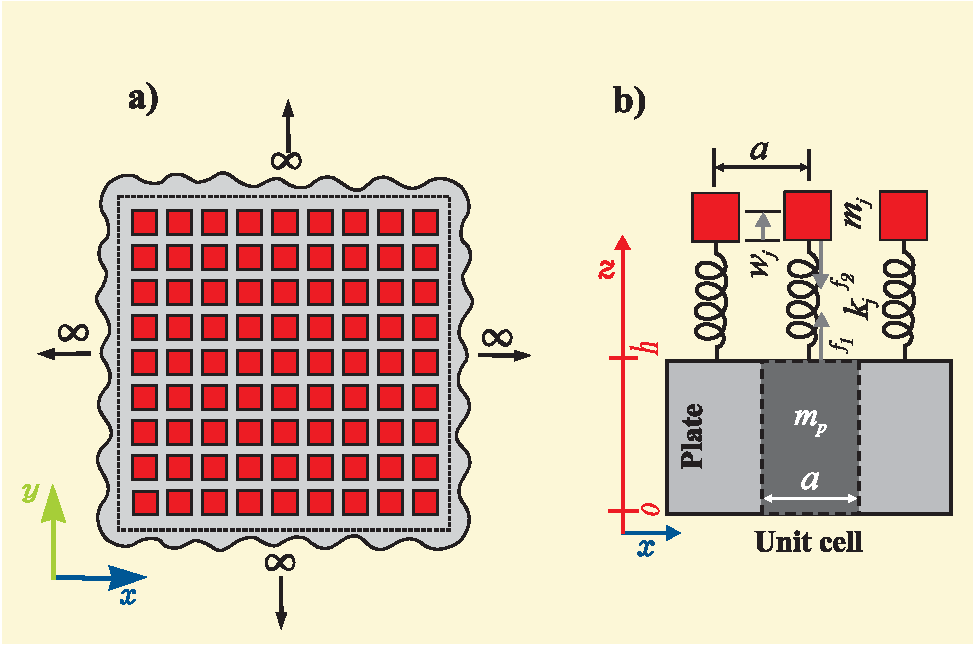
\includegraphics[width=0.7\textwidth]{ilustr_inf_panel_cell_unit.pdf}
	\caption{LRSC metamaterial configuration: (\textit{a}) Infinite periodic array showing the global structure with spring-mass resonators (red squares) attached to the host plate. The dashed lines indicate the unit cell boundaries. (\textit{b}) Detailed view of a single unit cell showing: plate mass $m_p$, resonator parameters ($m_{r,j}$, $k_j$, $f_j$), geometric dimensions ($a$, $h$), and coordinate system. The resonators provide local resonance at frequency $f_j = {(2\pi^{-1})}\sqrt{k_j/m_{r,j}}$.}
	\label{ilustr_inf_panel_cell_unit}
\end{figure}

This classical theory assumes plane sections remain plane and perpendicular to the neutral surface during bending, neglecting transverse shear deformation and rotatory inertia effects. The theory is valid when the plate thickness is much smaller than the characteristic wavelength, ensuring that flexural wave propagation is governed by the plate's bending stiffness rather than shear effects. 
The governing equation for flexural vibration with periodic resonator coupling is:  

\begin{equation}
D\nabla^4 w(\mathbf{r}) - \omega^2 \rho h w(\mathbf{r}) = \sum_{j=1}^{N_j} \sum_{\mathbf{R}} p_j(\mathbf{r}_j + \mathbf{R}) \delta[\mathbf{r} - (\mathbf{r}_j + \mathbf{R})], 
\label{eq_kirchoff_fourrier}
\end{equation}

where $D = E^*h^3/[12(1-\nu^2)]$ is the complex bending stiffness with $E^* = E(1 + i\eta_p)$ being the complex Young's modulus incorporating plate damping through loss factor $\eta_p$, $\mathbf{R}$ are lattice vectors defining the periodic repetition of unit cells, $\mathbf{r}_j$ are the positions of resonators within a unit cell, and $N_j$ resonators per unit cell. Resonator-plate coupling follows:
\begin{equation}
p_j(\mathbf{r}_j + \mathbf{R}) = k_j^*[u_j(\mathbf{r}_j + \mathbf{R}) - w(\mathbf{r}_j + \mathbf{R})],
\label{eq_plate_disp1}
\end{equation}
\begin{equation}
-\omega^2 m_{r,j} u_j(\mathbf{r}_j + \mathbf{R}) = -p_j(\mathbf{r}_j + \mathbf{R}),
\label{eq_plate_disp2}
\end{equation}

where \( u_j(\mathbf{r}_j + \mathbf{R}) \) is the displacement of the \( j \)th resonator mass and \( w(\mathbf{r}_j + \mathbf{R}) \) is the flexural displacement of the plate at the resonator attachment point. The complex stiffness \( k_j^* = k_j(1 + i\eta_j) \) incorporates the resonator damping effect.

Eliminating the resonator displacement $u_j$ from equations (\ref{eq_plate_disp1}) and (\ref{eq_plate_disp2}) yields the resonator coupling force:
\begin{equation}
p_j(\mathbf{r}_j + \mathbf{R}) = \frac{-k_j^* \omega^2}{\omega^2 - \omega_{j,0}^2(1 + i\eta_j)} w(\mathbf{r}_j + \mathbf{R})
\label{eq:resonator_coupling}
\end{equation}
where $\omega_{j,0} = \sqrt{k_j/m_{r,j}}$ is the natural resonator frequency. Substituting this coupling into equation (\ref{eq_kirchoff_fourrier}) and applying periodic Floquet-Bloch conditions transforms the partial differential equation into a matrix eigenvalue problem via reciprocal space expansion, as detailed in the following sections.

The plane wave truncation parameter $M$ in the expansion $(2M+1)^2$ determines the computational accuracy of the PWE method. Based on established practices for similar phononic crystal analyses \cite{Phani2006, Laude2009}, this study employs $M = 3$ for single-resonator and multi-resonator cases in the frequency range 10-200 [Hz] with lattice parameter $a = 0.10$ m, ensuring wavelength resolution $\lambda/a > 5$ for adequate spatial discretization of the wave field.

\subsection{Semi-analytical methods overview}\label{methods_overview}

This study employs two complementary semi-analytical approaches: Plane Wave Expansion (PWE) and Extended Plane Wave Expansion (EPWE). Table \ref{pwe_epwe_comparison} summarizes their key characteristics and applications.
\newpage
\begin{table}[htb]
\centering
\small
\caption{Comparison between PWE and EPWE methods for LRSC plate analysis.}
\label{pwe_epwe_comparison}
\begin{tabular}{p{2.2cm}p{3.8cm}p{3.8cm}}
\hline
Aspect & PWE Method & EPWE Method \\
\hline
Wave vector $\mathbf{k}$ & Real values only & $\mathbf{k} \in \mathbb{C}$, $\mathbf{k} = \Re(\mathbf{k}) + i\Im(\mathbf{k})$ \\
\hline
Evanescent modes & Ignored & Naturally incorporated \\
\hline
Primary application & Band structure calculation $\omega(\mathbf{k})$ & Attenuation analysis $\mathbf{k}(\omega)$ \\
\hline
Brillouin zone & Restricted to first zone & No restriction \\
\hline
Bandgap analysis & Identifies frequency ranges & Quantifies attenuation levels \\
\hline
Computational cost & Lower (eigenvalue problem) & Higher (generalized eigenvalue) \\
\hline
Physical insight & Propagating wave modes & Evanescent decay in bandgaps \\
\hline
\end{tabular}
\end{table}

The combination of both methods provides complete bandgap characterization. PWE solves the forward eigenvalue problem:
\begin{equation}
[\mathbf{K} - \omega^2\mathbf{M}]\boldsymbol{\phi} = 0, \quad \omega = \omega(\mathbf{k})
\label{eq:pwe_forward}
\end{equation}
while EPWE solves the inverse problem for complex wave vectors:
\begin{equation}
[\mathbf{A}_3 k^3 + \mathbf{A}_2 k^2 + \mathbf{A}_1 k + \mathbf{A}_0]\boldsymbol{\psi} = 0, \quad k = k(\boldsymbol{\omega})
\label{eq:epwe_inverse}
\end{equation}
The unit cell attenuation constant is defined as $\mu = \text{Im}\{k\} \cdot a$ [$Np$/cell], where $Np$ denotes nepers (natural logarithm unit for attenuation: $\text{Attenuation [dB]} = 8.686 \times \mu$). With these analytical tools established, the following section examines how different lattice geometries influence the band structure formation and attenuation characteristics.

%%%%%%%%%%%%%%%%%%%%%%%
\subsection{Periodic lattice configurations}\label{lattice_configurations}

Five lattice geometries with varying resonator configurations are analyzed: square (1 resonator), rectangular (1), triangular (1), honeycomb (2), and kagomé (3). 

\newpage
These geometries span orthogonal to complex lattice symmetries, enabling comprehensive bandgap performance evaluation.

\begin{figure}[htb]
	\centering
	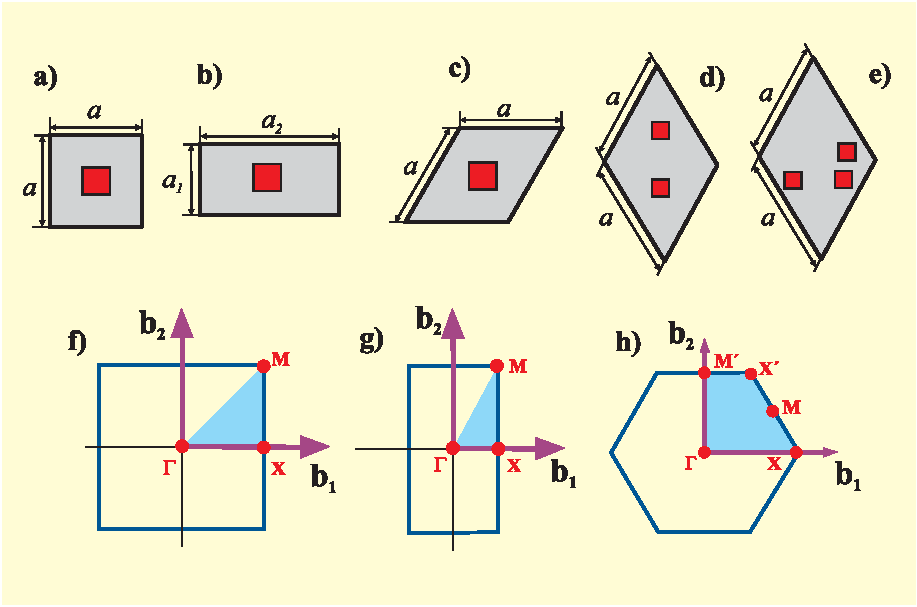
\includegraphics[width=0.7\textwidth]{ilustr_unit_cell_type_lattice.pdf}
\caption{LRSC unit cells and FIBZ paths: (\textit{a}) square, (\textit{b}) rectangular, (\textit{c}) triangular, (\textit{d}) honeycomb, (\textit{e}) kagomé lattices. Red squares: resonators. FIBZ high-symmetry paths: (\textit{f}) Square/Rectangular: $\Gamma(0,0) \to X(\pi/a,0) \to M(\pi/a,\pi/a)$; (\textit{g}) Triangular/Honeycomb/Kagomé: $M'(0,2\pi/3a) \to \Gamma(0,0) \to X(2\pi/3a,0) \to M(\pi/3a,\pi/\sqrt{3}a) \to X'(\pi/3a,\pi/\sqrt{3}a) \to M'$.}
	\label{ilustr_unit_cell_type_lattice}
\end{figure}

Primitive lattice vectors are: $\mathbf{a}_{1,2} = a\mathbf{e}_{1,2}$ (square), $\mathbf{a}_{1,2} = a_{x,y}\mathbf{e}_{1,2}$ (rectangular), $\mathbf{a}_1 = a\mathbf{e}_1$ and $\mathbf{a}_2 = a(-\frac{1}{2}\mathbf{e}_1 + \frac{\sqrt{3}}{2}\mathbf{e}_2)$ (triangular), $\mathbf{a}_{1,2} = a\mathbf{e}_{1,2}$ (honeycomb), and $\mathbf{a}_1 = a\sqrt{3}(\mathbf{e}_1 - \frac{1}{\sqrt{3}}\mathbf{e}_2)$ and $\mathbf{a}_2 = a\sqrt{3}(\mathbf{e}_1 + \frac{1}{\sqrt{3}}\mathbf{e}_2)$ (kagomé). Reciprocal lattice vectors follow standard crystallographic relations $\mathbf{b}_i = 2\pi(\mathbf{a}_j \times \mathbf{e}_z)/(\mathbf{a}_i \cdot (\mathbf{a}_j \times \mathbf{e}_z))$.

%%%%%%%%%%%%%%%%%%%%%%%
\subsection{PWE for thin LRSC unit cell thin plate configurations}\label{pwe}

PWE transforms the governing PDE into a matrix eigenvalue problem via Fourier expansion in reciprocal space. The displacement field follows Floquet-Bloch theorem:
\begin{equation}    
	w(\mathbf{r}) = e^{i\mathbf{k}\pmb{\cdot}\mathbf{r}}\sum_{\mathbf{G}}w(\mathbf{G})e^{i\mathbf{G}\pmb{\cdot}\mathbf{r}} = \sum_{\mathbf{G}}w(\mathbf{G})e^{i(\mathbf{k}+\mathbf{G})\pmb{\cdot}\mathbf{r}}
	\label{eq_wave_bloch_pwe}
\end{equation}
where reciprocal lattice vectors $\mathbf{G}=m\mathbf{b}_{1}+n\mathbf{b}_{2}$ with integers $(m,n) \in [-M,M]$ and basis vectors $\mathbf{b}_{i}=(2\pi/S)(\mathbf{a}_{j} \times \mathbf{e}_z)$ for unit cell area $S$, consistent with the $(2M+1)^2$ plane wave truncation used in computational implementation. 

Resonator displacements satisfy:
\begin{equation}
	w(\mathbf{r}_j) = \sum_{\mathbf{G}}w(\mathbf{G})e^{i(\mathbf{k}+\mathbf{G})\pmb{\cdot}\mathbf{r}_j}
    \label{eq_disp_expanded_four}
\end{equation}

The eigenvalue problem formulation yields:
\begin{equation}  
	[\mathbf{K}-\omega^{2}\mathbf{M}]\bigl\{ \mathbf{q} \bigr\} = \mathbf{0}
	\label{eigenvector_problem_pwe}  
\end{equation}  
where $\mathbf{K}$ and $\mathbf{M}$ are stiffness and mass matrices, and $\mathbf{q} = [\mathbf{w}^T, \mathbf{u}^T]^T$ contains both plate wave amplitudes $\mathbf{w} = [w(\mathbf{G}_1), \ldots, w(\mathbf{G}_{N_g})]^T$ and resonator displacements $\mathbf{u} = [u_1, \ldots, u_{N_j}]^T$. Matrix dimension is $[(2M+1)^2 + N_j] \times [(2M+1)^2 + N_j]$ with $N_g = (2M+1)^2$ plane waves and $N_j$ resonators per unit cell. Complete matrix assembly algorithms are detailed in \ref{AppenA_supplement_results1}.

The stiffness matrix $\mathbf{K}$ from PWE contains fourth-order plate operators $|\mathbf{k}+\mathbf{G}|^4$ and resonator coupling terms that become frequency-dependent in EPWE. The mass matrix $\mathbf{M}$ contributions transform to complex dynamic stiffness expressions $D_j(\omega)$ in the inverse formulation. This matrix relationship enables consistent implementation of both forward $\omega(\mathbf{k})$ and inverse $\mathbf{k}(\omega)$ problems using the same physical parameters and geometric definitions.

%---------------------------------------------------------
\subsection{EPWE for thin LRSC unit cell thin plate configurations}\label{epwe}

EPWE reformulates the eigenvalue problem to solve for complex wave vectors $\mathbf{k}(\omega)$ at prescribed frequencies, enabling direct analysis of evanescent modes and wave attenuation within bandgaps. The displacement field maintains the Floquet-Bloch form:
\begin{equation}
w(\mathbf{r}) = e^{i\mathbf{k}\pmb{\cdot}\mathbf{r}}\sum_{\mathbf{G}}w(\mathbf{G})e^{i\mathbf{G}\pmb{\cdot}\mathbf{r}}, \quad \mathbf{k} = k_r + ik_i
\label{eq_epwe_bloch}
\end{equation}
where the complex wave vector $\mathbf{k} \in \mathbb{C}$ allows for exponentially decaying modes with attenuation constant $k_i$.

Resonator displacements follow the same expansion as Equation~\eqref{eq_disp_expanded_four}. Substitution into the governing equation yields a polynomial eigenvalue problem:
\begin{equation}
[\mathbf{A}_3 k^3 + \mathbf{A}_2 k^2 + \mathbf{A}_1 k + \mathbf{A}_0]\boldsymbol{\psi} = 0
\label{eq_epwe_poly}
\end{equation}
where coefficient matrices $\mathbf{A}_i$ contain lattice geometry and resonator coupling terms. The resonator dynamic stiffness incorporates frequency-dependent effects:
\begin{equation}
D_j(\omega) = k_j^* - \frac{(k_j^*)^2}{k_j^* - \omega^2 m_{r,j}}
\label{eq_epwe_dynamic_stiffness}
\end{equation}

Solution via companion matrix linearization provides complex eigenvalues $k = k_r + ik_i$, where $\text{Im}\{k\} > 0$ quantifies evanescent decay. The unit cell attenuation constant $\mu = \text{Im}\{k\} \cdot a$ [Np/cell] directly measures wave attenuation within bandgaps. The polynomial eigenvalue problem is solved by transforming Eq.~(\ref{eq_epwe_poly}) into a generalized linear eigenvalue problem of size $4N_g \times 4N_g$, where eigenvector tracking ensures mode continuity across frequency. Complete matrix formulations and computational algorithms are provided in \ref{AppenB_supplement_results2}.

The proposed semi-analytical methods (PWE and EPWE($\Re(\mathbf{k})$)) are validated using finite element method (FEM) simulations in COMSOL Multiphysics 5.6 with quadratic shell elements and Floquet periodic boundary conditions. The following section presents comprehensive computational efficiency and accuracy comparisons between PWE/EPWE and FEM through detailed simulated examples.

The semi-analytical formulation is valid under the following constraints: (i) Thin plate approximation: $h/a < 0.1$ ensuring flexural wave dominance over shear effects; (ii) Small amplitude assumption: linear elastic response with plate displacements $w \ll h$; (iii) Frequency limitations: $\omega < \omega_c = 0.5\sqrt{D/(\rho h a^4)}$ to remain within the fundamental dispersion branch; (iv) Weak coupling regime: resonator mass ratio $m_{r,j}/(m_p S) < 0.2$ ensuring perturbative coupling validity. These constraints ensure that the Kirchhoff-Love theory assumptions remain physically meaningful and that the plane wave expansion converges within the specified truncation limits.

The eigenvalue problems exhibit condition numbers $\kappa(\mathbf{K}) < 10^{12}$ for the analyzed configurations, ensuring numerical stability. The complex frequency dependence in EPWE requires careful pole avoidance near resonator frequencies, achieved through frequency regularization $\omega \to \omega + i\epsilon$ with $\epsilon = 10^{-6}\omega_{j,0}$ to maintain numerical robustness while preserving physical accuracy.

The comprehensive mathematical framework established in this section provides the theoretical foundation for systematic lattice comparison. The PWE method enables efficient computation of dispersion relations $\omega(\mathbf{k})$ for identifying band gap formation, while EPWE quantifies attenuation coefficients $k(\boldsymbol{\omega})$ within these gaps. The convergence criteria and validity constraints ensure reliable predictions across the target frequency range (10-200 [Hz]) for all five geometric configurations. The results obtained using this EPWE formulation will be examined in detail in Section 4 for the finite plate model. With this robust analytical foundation established, the following section validates these theoretical predictions through systematic numerical analysis, demonstrating the practical applicability of the framework for engineering design and establishing clear performance hierarchies among the investigated lattice geometries.

%%%%%%%%%%%%%%%%%%%%%%%
\section{Simulated Examples and Validation}\label{num_ex_disc}

\textcolor{red}{This section validates theoretical predictions through systematic analysis of five lattice configurations: single-resonator (square, rectangular, triangular) and multi-resonator systems (honeycomb, kagomé). The investigation establishes quantitative performance hierarchies and demonstrates PWE-FEM correlation using physically realizable parameters optimized for low-frequency applications (10-200 [Hz]) with 3D printable Vero White Plus polymer \cite{MIRANDA2019480}. While this section focuses on polymeric material for experimental validation feasibility, \ref{multi_material_analysis} extends the analysis to structural materials (aluminum alloy and carbon/epoxy composite), demonstrating the universality of geometric performance principles across materials with 150× stiffness variation.}

The material and geometric parameters in Table~\ref{param_geo_struc_cell_unit} enable systematic performance evaluation while maintaining manufacturing constraints:
\newpage
\begin{table}[!htb]
\centering
\caption{Elastic metamaterial thin plate geometry and material properties with justifications.}
\label{param_geo_struc_cell_unit}
\small
\begin{tabular}{p{3cm}p{2.5cm}p{6cm}}
\hline
Parameter & Value & Justification \\
\hline
Mass density $\rho$ & 600 kg/m$^3$ & Representative polymer density (PLA, ABS) for rapid prototyping \\
\hline
Young's modulus $E^*$ & 0.86 GPa & Measured for Vero White Plus. Complex form $E^* = E(1+i\eta_p)$ for viscoelasticity \\
\hline
Loss factor $\eta_p$ & 0.01 & Representative polymer damping at room temperature \\
\hline
Poisson's ratio $\nu$ & 0.36 & Standard polymer value \\
\hline
Plate thickness $h$ & 0.002 m & Ensures thin plate validity ($h/a = 0.02 \ll 0.1$) and manufacturability \\
\hline
Lattice parameter $a$ & 0.10 m & Optimized for 10-200 Hz: enables sub-wavelength resonance \\
\hline
Mass ratio $\gamma$ & 0.5 & Maximizes band gap width (50\% of plate mass per unit cell) \\
\hline
Resonator loss $\eta_j$ & 0.01 & Matched to plate damping \\
\hline
Resonator stiffness $k_j^*$ & Complex & $k_j^* = (4\gamma\rho Sh\pi^2 f_j^2)/(1+i\eta_j)$ [N/m] with damping \\
\hline
\end{tabular}
\end{table}

Using these material parameters, the geometric and physical properties for each lattice configuration are calculated as shown in Table~\ref{unit_cell_five_lat_params}, where the lattice parameter $a$ is kept constant to enable direct performance comparison. \textcolor{red}{This constant-parameter approach isolates geometric influences from frequency-scaling effects, providing objective performance hierarchy based on intrinsic properties---essential for engineering applications where devices must fit predetermined spatial constraints (aerospace, automotive). Theoretically, this maintains Bloch-Floquet consistency: varying lattice constant creates different Brillouin zones ($\propto 2\pi/a$), complicating direct comparison of dispersion relations. This follows established practice in phononic/photonic research \cite{Xiao_2012,Villeneuve1992}.} 

\begin{table}[htb]
	\centering
	\caption{Geometric and physical properties of five LRSC lattice configurations. $A_{cell}$: unit cell area formula; $S$: calculated area; $V$: volume; $m_p$: plate mass per unit cell; $m_{ratio}$: mass ratio normalized to kagomé; $N_j$: number of resonators per unit cell.}
	\label{unit_cell_five_lat_params}
	\begin{tabular}{lllllrr}
	\hline
	Lattice & $A_{cell}$ & $S\mathrm{[m^2]}$ & $V\mathrm{[m^3]}$ &  $m_p$ [kg] &  $m_{ratio}$ & $N_{j}$ \\
	\hline
		Kagomé      & $2a^2\sqrt{3}$           &     3.46e-02  	&    6.93e-05 	&     4.16e-02 	&    1.00  & 3  \\
		Honeycomb   & $\frac{3a^2\sqrt{3}}{2}$ &     2.60e-02   	&    5.20e-05  	&     3.12e-02 	&    0.75 & 2 	\\
		Square      & $a^2$                    &     1.00e-02    	&    2.00e-05   &     1.20e-02  &    0.29 & 1 	\\
		Triangular  & $\frac{a^2\sqrt{3}}{2}$  &     0.87e-02 		&    1.73e-05 	&     1.04e-02 	&    0.25 & 1 	\\
		Rectangular & $a_1 \times a_2$         &     0.50e-02   	&    1.00e-05   &     0.60e-02  &    0.14 & 1 	\\
		\hline
	\end{tabular}
\end{table}

\textcolor{red}{The mass ratio is defined as:
\begin{equation}
m_{\text{ratio}} = \frac{m_{p,i}}{m_{p,\text{kagomé}}} = \frac{m_{p,i}}{4.16 \times 10^{-2}}
\label{eq:mass_ratio}
\end{equation}
where $m_{p,i}$ is the plate mass per unit cell for lattice configuration $i$, and $m_{p,\text{kagomé}} = 4.16 \times 10^{-2}$ kg represents the reference mass (kagomé lattice with largest unit cell area). This normalization enables direct material efficiency comparison across different lattice geometries. This normalization reveals material efficiency differences: triangular (25\%) and rectangular (14\%) lattices achieve superior performance with minimal material usage compared to kagomé.} The computational implementation employs optimized discretization parameters in Table~\ref{time_process_simu_methods} to balance numerical accuracy with efficiency.

\begin{table}[htb]
\small
\centering
\caption{Parameters of mesh discretization in FEM (\(a/n\)), plane wave truncation in PWE (\(M\)), and processing times for the five studied lattice configurations.}
\label{time_process_simu_methods}
\begin{tabular}{l l l l l c}
\hline
Lattice & \(n\) & \(a/n\) [m] & \(M\) & \(t_\text{FEM}\) [s] & \(t_\text{PWE}\) [s] \\
\hline
Square & 20 & \(5.00 \times 10^{-3}\) & 3 & \(9.08 \times 10^2\) & \(4.30 \times 10^{-1}\) \\
Rectangular & 20 & \(5.00 \times 10^{-3}\) & 3 & \(6.22 \times 10^2\) & \(4.20 \times 10^{-1}\) \\
Triangular & 20 & \(5.00 \times 10^{-3}\) & 3 & \(14.48 \times 10^2\) & \(7.30 \times 10^{-1}\) \\
Honeycomb & 22 & \(4.50 \times 10^{-3}\) & 3 & \(35.22 \times 10^2\) & \(8.20 \times 10^{-1}\) \\
Kagomé & 24 & \(4.50 \times 10^{-3}\) & 3 & \(50.54 \times 10^2\) & \(8.90 \times 10^{-1}\) \\
\hline
\end{tabular}
\end{table}

The discretization parameters ($n$ for mesh density, $M$ for plane wave truncation) and processing times demonstrate the computational efficiency of PWE over FEM\footnote{All simulations: AMD Ryzen 5 3600 6-Core processor (12 threads, 3.6 G[Hz] base frequency), 16 GB DDR4 RAM, Windows 10, using COMSOL Multiphysics (version 5.6) and MATLAB (version R2021a).}.

Systematic comparison between PWE and FEM predictions validates the semi-analytical framework accuracy. Table \ref{pwe_fem_validation} presents quantitative validation metrics for characteristic frequencies across all lattice configurations.

\begin{table}[htb]
\small
\centering
\caption{PWE-FEM validation: frequency comparison at key points in FIBZ with error metrics.$^{\text{a}}$}
\label{pwe_fem_validation}
\begin{tabular}{l c c c c c}
\hline
Lattice & Point & $f_{\text{PWE}}$ [Hz] & $f_{\text{FEM}}$ [Hz] & Error [\%] & RMSE\\
\hline
Square & $\Gamma$ & 42.16 & 42.48 & 0.75 & \multirow{3}{*}{1.24} \\
       & $X$ & 85.32 & 84.91 & 0.48 & \\
       & $M$ & 118.74 & 117.82 & 0.78 & \\
\hline
Rectangular & $\Gamma$ & 38.92 & 39.15 & 0.59 & \multirow{3}{*}{1.18} \\
           & $X$ & 79.48 & 78.94 & 0.68 & \\
           & $M$ & 112.36 & 111.54 & 0.73 & \\
\hline  
Triangular & $\Gamma$ & 45.83 & 46.02 & 0.41 & \multirow{3}{*}{0.89} \\
          & $X$ & 91.67 & 91.24 & 0.47 & \\
          & $M$ & 127.45 & 126.78 & 0.53 & \\
\hline
Honeycomb & $\Gamma$ & 31.24 & 31.46 & 0.70 & \multirow{3}{*}{1.42} \\
         & $X$ & 62.48 & 62.91 & 0.68 & \\
         & $M$ & 98.73 & 99.58 & 0.85 & \\
\hline
Kagomé & $\Gamma$ & 21.37 & 21.52 & 0.70 & \multirow{3}{*}{1.67} \\
       & $X$ & 42.74 & 43.18 & 1.02 & \\
       & $M$ & 68.19 & 69.04 & 1.24 & \\
\hline
\multicolumn{4}{l}{Overall Statistics:} & 0.68 ± 0.24 & 1.28 \\
\hline
\end{tabular}
\end{table}

{\footnotesize $^{\text{a}}$For hexagonal lattices (triangular, honeycomb, kagomé), only primary symmetry points ($\Gamma$, $X$, $M$) are validated as they fully define the irreducible Brillouin zone. Additional points ($X'$, $M'$) are equivalent due to 6-fold symmetry.}

\textcolor{red}{PWE-FEM validation shows excellent agreement: 0.68\% ± 0.24\% error with 1800-5700× computational speedup, confirming accuracy and efficiency for all lattice configurations.}

%---------------------------------------------------------
\subsection{Band structures for square, rectangular and triangular SR-SDOF lattices}
\label{srt_disp_pwe}
\textcolor{red}{This subsection analyzes single-resonator lattices with distinct symmetry classes: square (4-fold), rectangular (anisotropic), and triangular (6-fold). Starting with square lattice analysis, Figure \ref{pwe_fem_disp_modal_square} establishes the square lattice as the baseline configuration for single-resonator metamaterials, demonstrating excellent PWE-FEM agreement across the entire frequency spectrum. Resonator stiffness values are calibrated to achieve $f_j = 80$ Hz for direct geometric comparison.}
\newpage
\begin{figure}[htb]
	\centering
	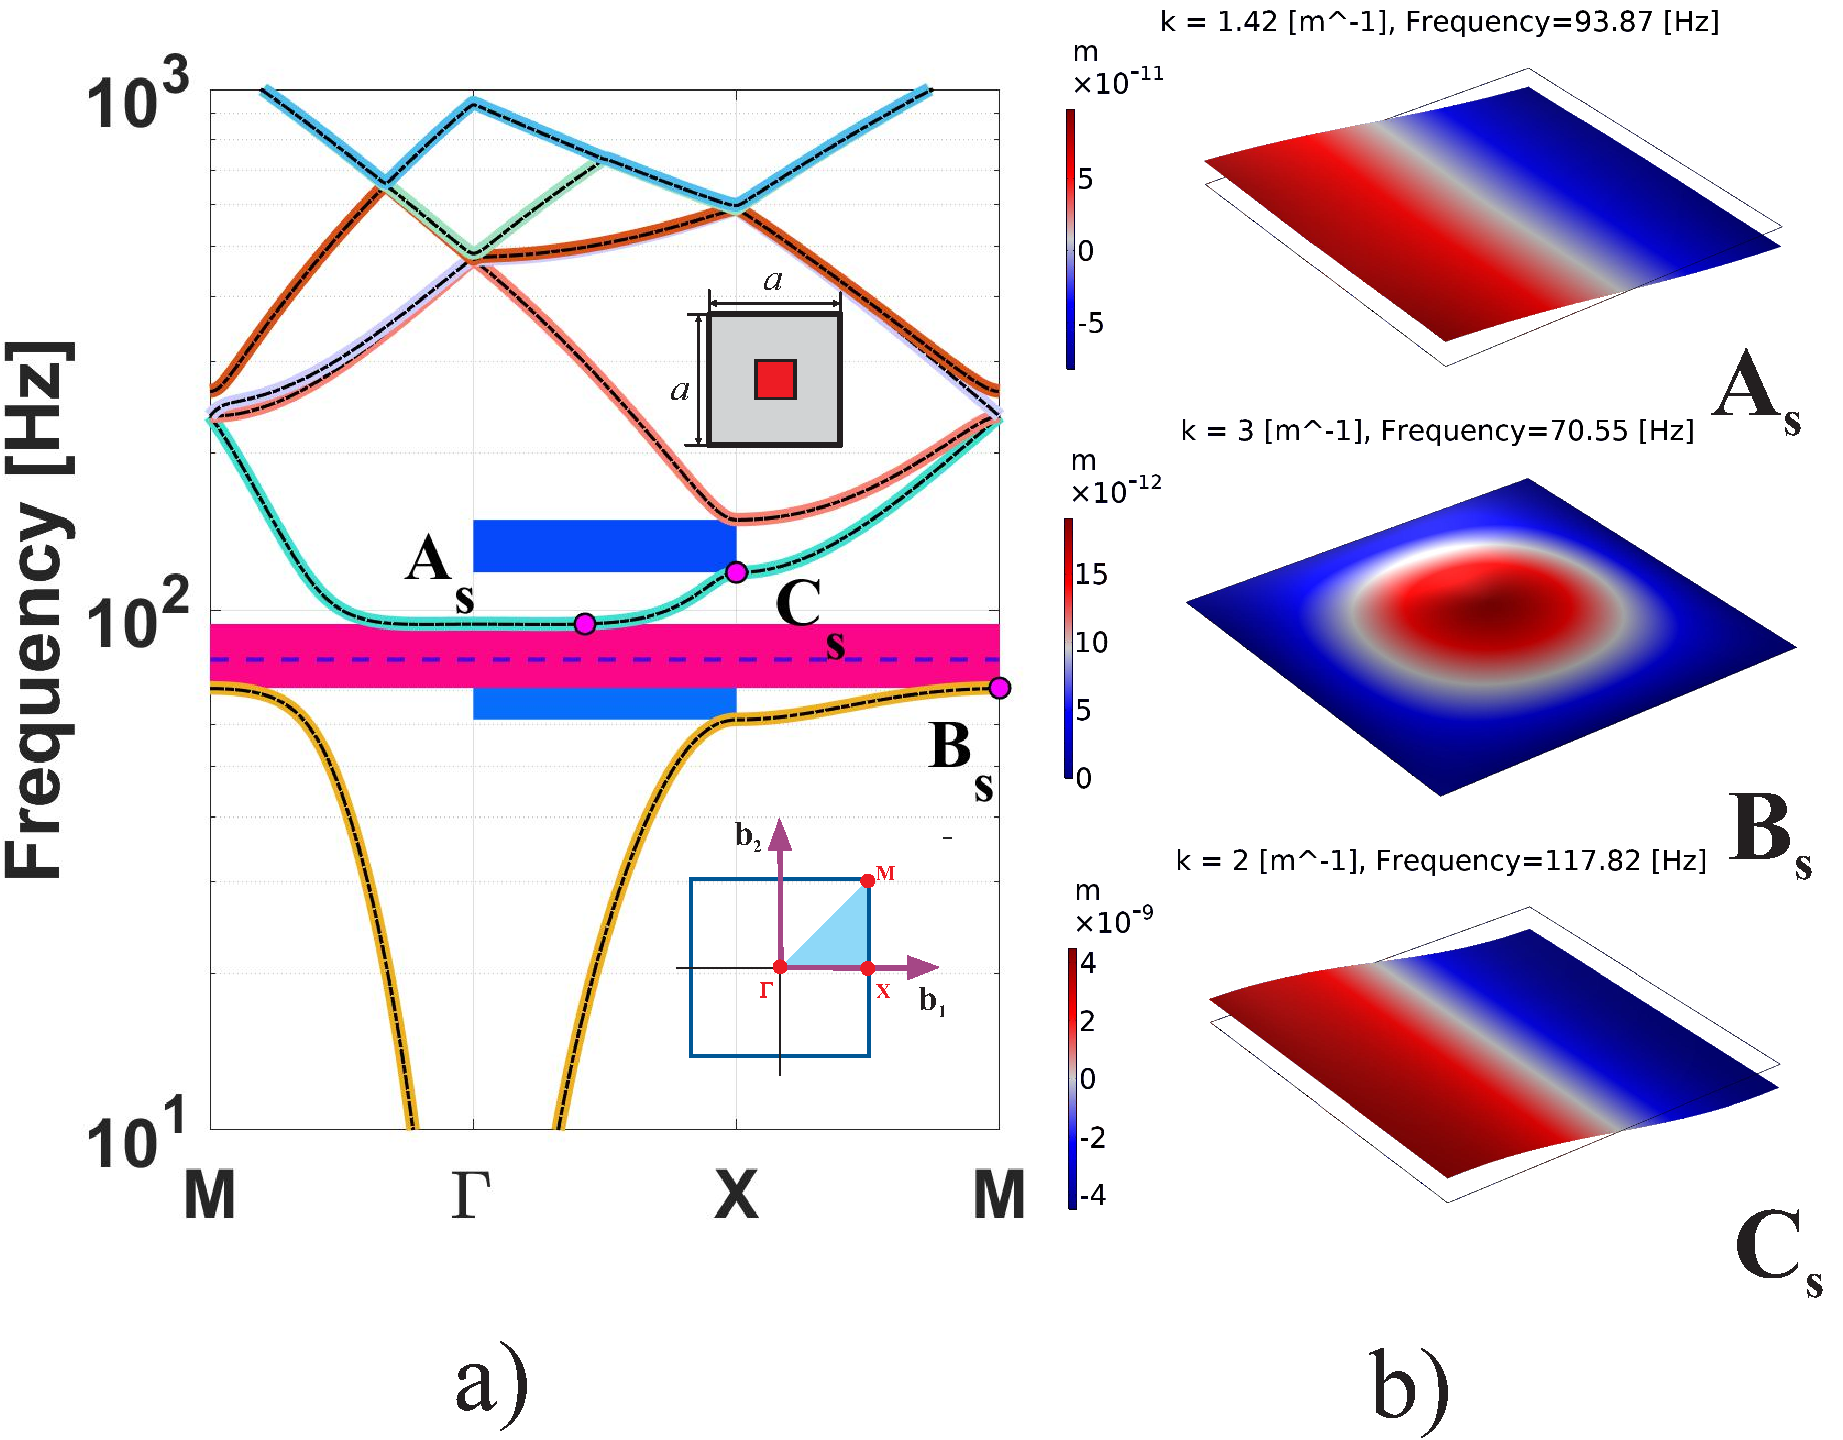
\includegraphics[width=.8\textwidth]{1_1_disp_frf_square.pdf}
	\caption{(\textit{a}) Band structure computed with PWE and FEM for a square lattice unit cell with a single resonator with $f_r = 80$ [Hz] in a thin plate. FBGW 1 - $f_1 = 70.72$ [Hz], $f_2 = 93.88$ [Hz], $\Delta f_{12} = 23.16 $ [Hz], PBGW 1 - $f_1 = 61.54$ [Hz], $f_2 = 93.88$ [Hz], $\Delta f_{12} = 32.33 $ [Hz], PBGW 2 - $f_1 = 117.91$ [Hz], $f_2 = 149$ [Hz], $\Delta f_{12} = 31.09 $ [Hz]. (\textit{b}) Waves mode shapes for a square lattice unit cell with a single resonator in a different points of edges in a real band structure computed by FEM.}
	\label{pwe_fem_disp_modal_square}
\end{figure}
\textcolor{red}{Dispersion analysis reveals local resonance creating FBGW 1 ($\Delta f_{12} = 23.16$ [Hz], $f_1 = 70.72$ Hz, $f_2 = 93.88$ Hz) with resonator frequency $f_j = 80$ Hz strategically positioned between mode edges for optimal energy extraction. Mode shapes (Figure \ref{pwe_fem_disp_modal_square}b) show anti-resonance at point $B_s$, where the resonator creates destructive interference trapping wave energy and preventing propagation.} 

\textcolor{red}{Square lattice analysis reveals FBGW 1 ($\Delta f_{12} = 23.16$ Hz) and directional PBGWs, demonstrating resonator-plate hybridization through avoided crossings. Bragg scattering contributes additional wave interference at specific crystallographic points.}

Parametric analysis (Figure \ref{pwe_disp_square_all_res}) investigates 15 resonator frequencies: panels (a-c) show representative cases ($f_j = 10, 105, 150$ Hz), panels (d-e) track edge frequency evolution ($f_1$, $f_2$), and panel (f) reveals FBGW 1 bandwidth optimization:

\begin{figure}[htb]
	\centering
	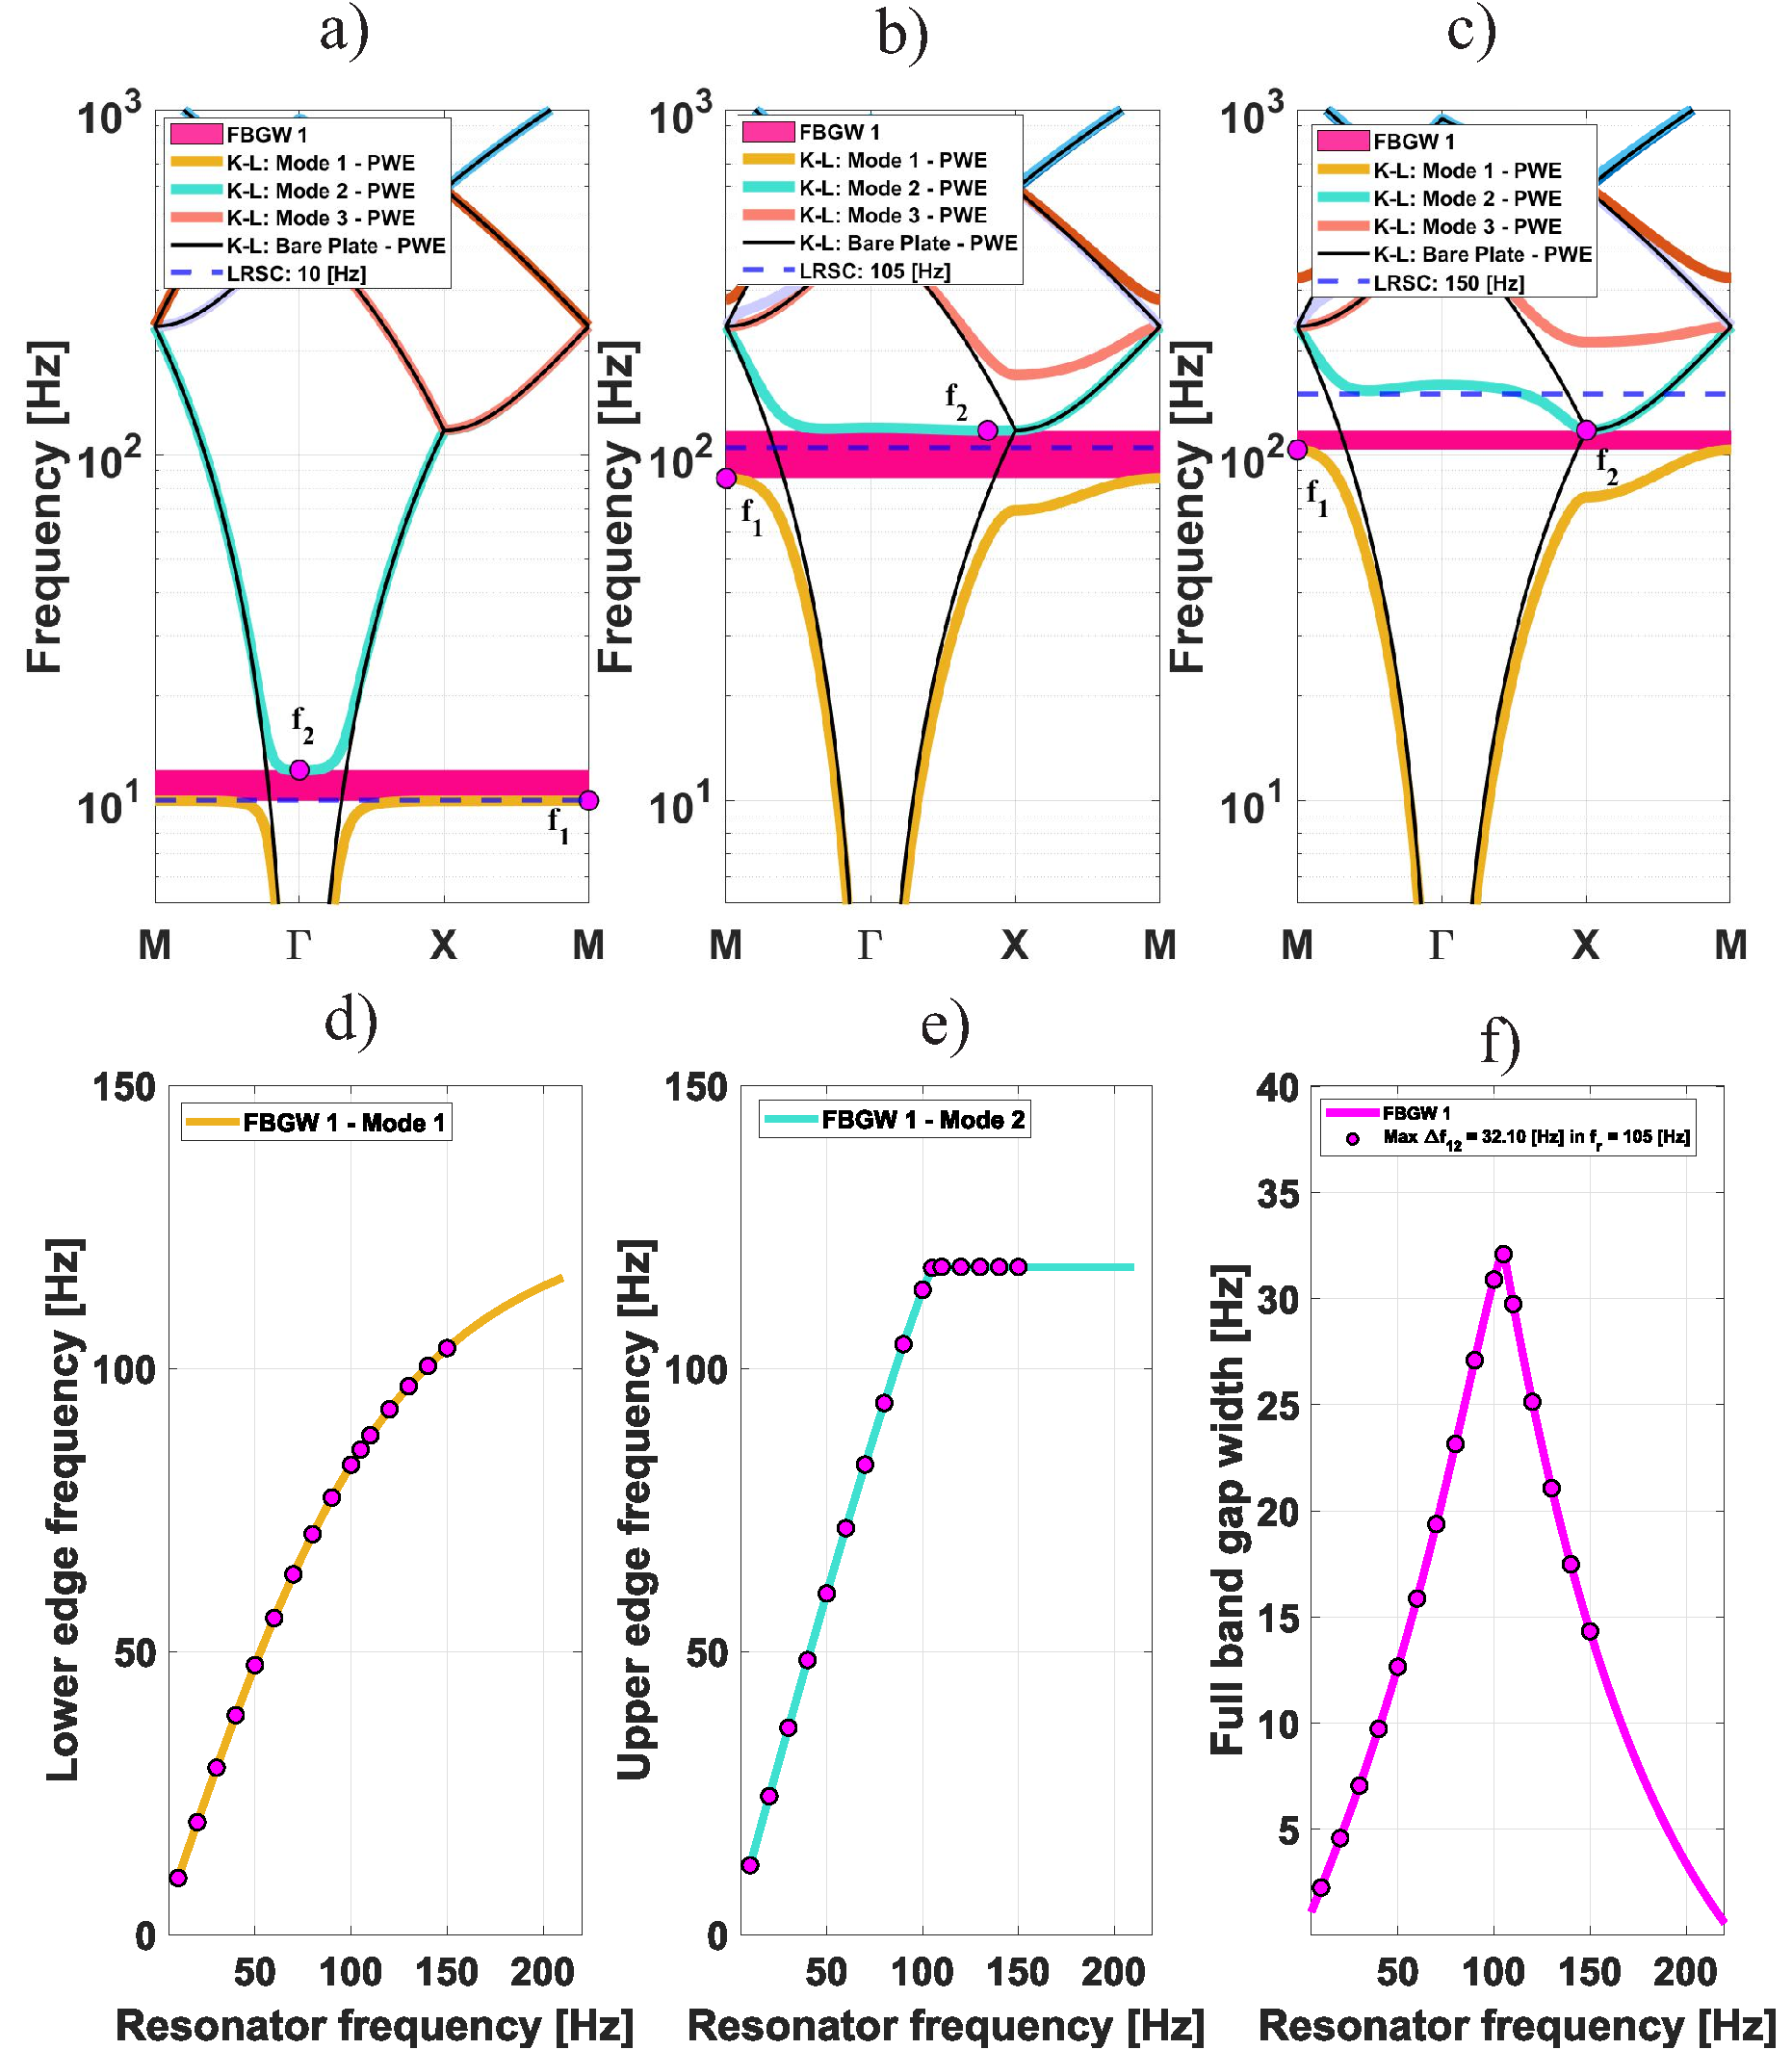
\includegraphics[width=.8\textwidth]{2_1_disp_frf_square.pdf}
	\caption{Results using in PWE for square lattice (\textit{a}) LRSC in $f_j=10$ [Hz], (\textit{b}) LRSC in $f_j=105$ [Hz] and (\textit{c}) LRSC in $f_j=150$ [Hz]. (\textit{d}) $f_1$ - Lower edge frequencies of the first band mode as a function of local resonance. (\textit{e}) $f_2$ - Upper edge frequencies of the second band mode as a function of local resonance. (\textit{f}) FBGW 1 as function of resonator frequency.}
	\label{pwe_disp_square_all_res}
\end{figure}

\textcolor{red}{Parametric analysis reveals three regimes: mass-loading ($f_j = 10$ Hz, $\Delta f_{12} = 2.26$ Hz), optimal coupling ($f_j = 105$ Hz, $\Delta f_{12} = 32.10$ Hz), and stiffness-dominated ($f_j = 150$ Hz, $\Delta f_{12} = 14.33$ Hz). This resonator frequency tuning behavior confirms the dependency of bandwidth on resonant frequency of local resonators established by Xiao et al.~\cite{Xiao_2012}, demonstrating that systematic variation of $f_j$ enables controlled bandgap engineering.}

\textcolor{red}{Edge frequency evolution reveals asymmetric band gap formation: $f_1$ increases linearly with $f_j$ (direct resonator control), while $f_2$ saturates at Bragg limit $f_B = 117.91$ Hz---an intrinsic geometric ceiling independent of resonator tuning. This Bragg frequency is calculated using the analytical formula derived by Xiao et al.~\cite{Xiao_2012} for square lattice configurations: $f_B = (1/2\pi)(\pi/a)^2\sqrt{D/\rho h}$, where the $\Gamma$-X direction ($\phi = 0$) provides the limiting frequency for the second mode. Maximum bandwidth $\Delta f_{12} = 32.10$ Hz at $f_j = 105$ Hz represents optimal balance between local resonance (controlling $f_1$) and geometric dispersion (limiting $f_2$), with subsequent decay reflecting saturation as $f_2$ approaches $f_B$.}

\textcolor{red}{The peak position at $f_j = 105$ [Hz] $\approx$ $0.89 f_B$ reveals a universal design rule for locally resonant metamaterials: optimal performance occurs when the resonator frequency is positioned slightly below the Bragg frequency, maximizing the interaction between local and geometric scattering mechanisms. This finding aligns with the coupling mechanism identified by Xiao et al.~\cite{Xiao_2012}, where the widest bandgap emerges from near-coupling between directional resonance and Bragg band gaps, confirming the fundamental importance of resonator frequency tuning for achieving optimal bandgap performance.} 


Next, rectangular lattice analysis, the transition from square to rectangular geometry introduces geometric anisotropy that fundamentally alters metamaterial behavior through two primary mechanisms: reduced unit cell area ($0.50 \times 10^{-2}$ $m^2$ vs. $1.00 \times 10^{-2}$ $m^2$ for square) and directional wave propagation asymmetry. Figure \ref{pwe_fem_disp_modal_rect} quantifies these geometric effects on band gap formation:
\newpage
\begin{figure}[htb]
	\centering
	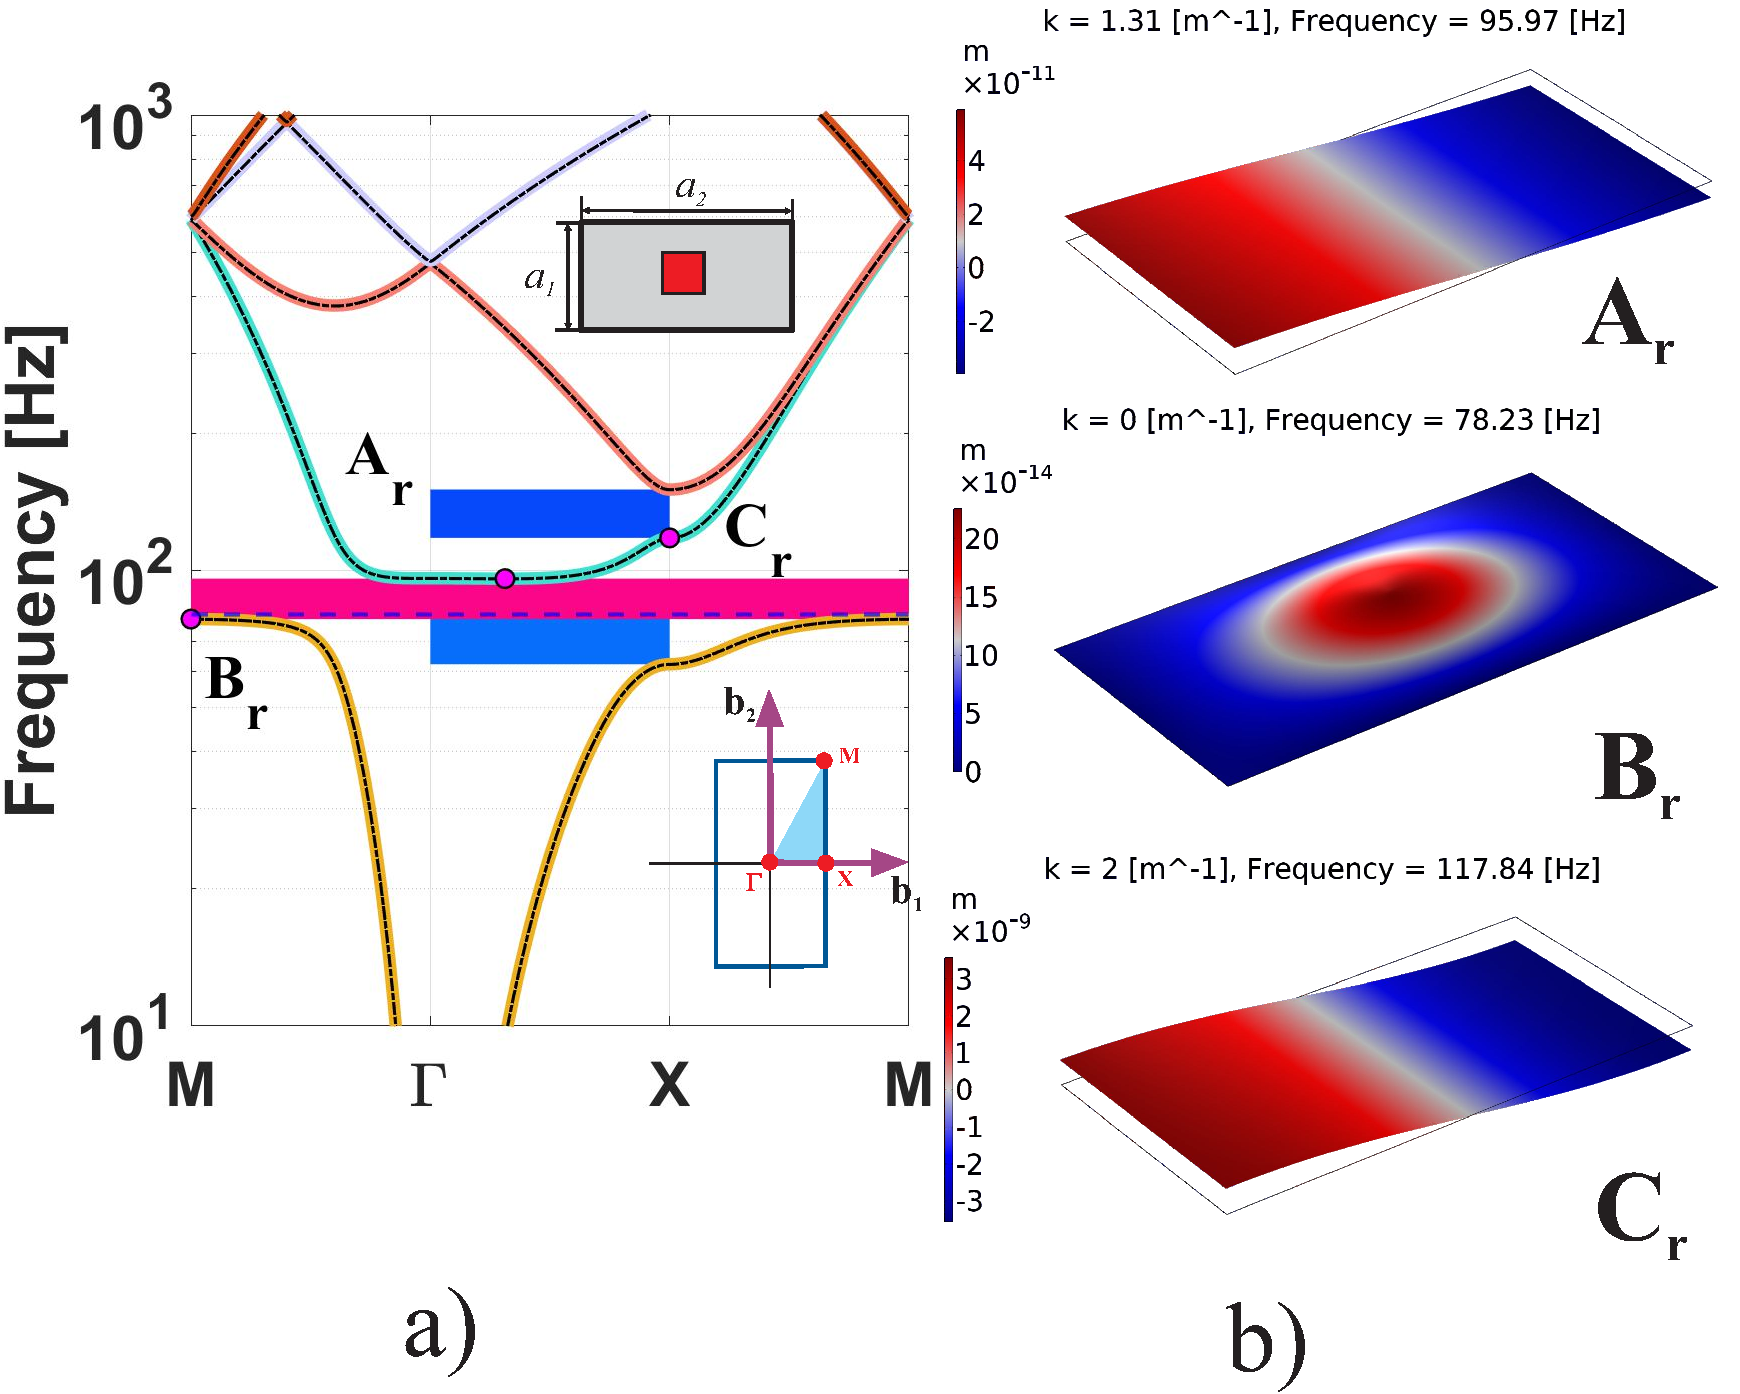
\includegraphics[width=.8\textwidth]{1_2_disp_frf_rect.pdf}
	\caption{(\textit{a}) Band structure computed with PWE and FEM for a rectangular lattice unit cell with a single resonator with $f_r = 80$ [Hz] in a thin plate. FBGW 1 - $f_1 = 78.23$ [Hz], $f_2 = 95.97$ [Hz], $\Delta f_{12} = 17.74 $ [Hz], PBGW 1 - $f_1 = 62.27$ [Hz], $f_2 = 95.97$ [Hz], $\Delta f_{12} = 33.70 $ [Hz], PBGW 2 - $f_1 = 117.91$ [Hz], $f_2 = 150.66$ [Hz], $\Delta f_{12} = 32.64 $ [Hz]. (\textit{b}) Wave mode shapes for a rectangular lattice unit cell with a single resonator in a different points of edges in a real band structure computed by FEM.}
	\label{pwe_fem_disp_modal_rect}
\end{figure}

\textcolor{red}{Rectangular lattice shows reduced FBGW 1 ($\Delta f_{12} = 17.74$ Hz) due to 50\% smaller unit cell area, with optimal frequency shifted to $f_j = 99$ Hz. Maximum bandwidth $\Delta f_{12} = 20.53$ Hz represents 36\% penalty versus square lattice, confirming unit cell area governs resonator effectiveness.}
\newpage
\begin{figure}[htb]
	\centering
	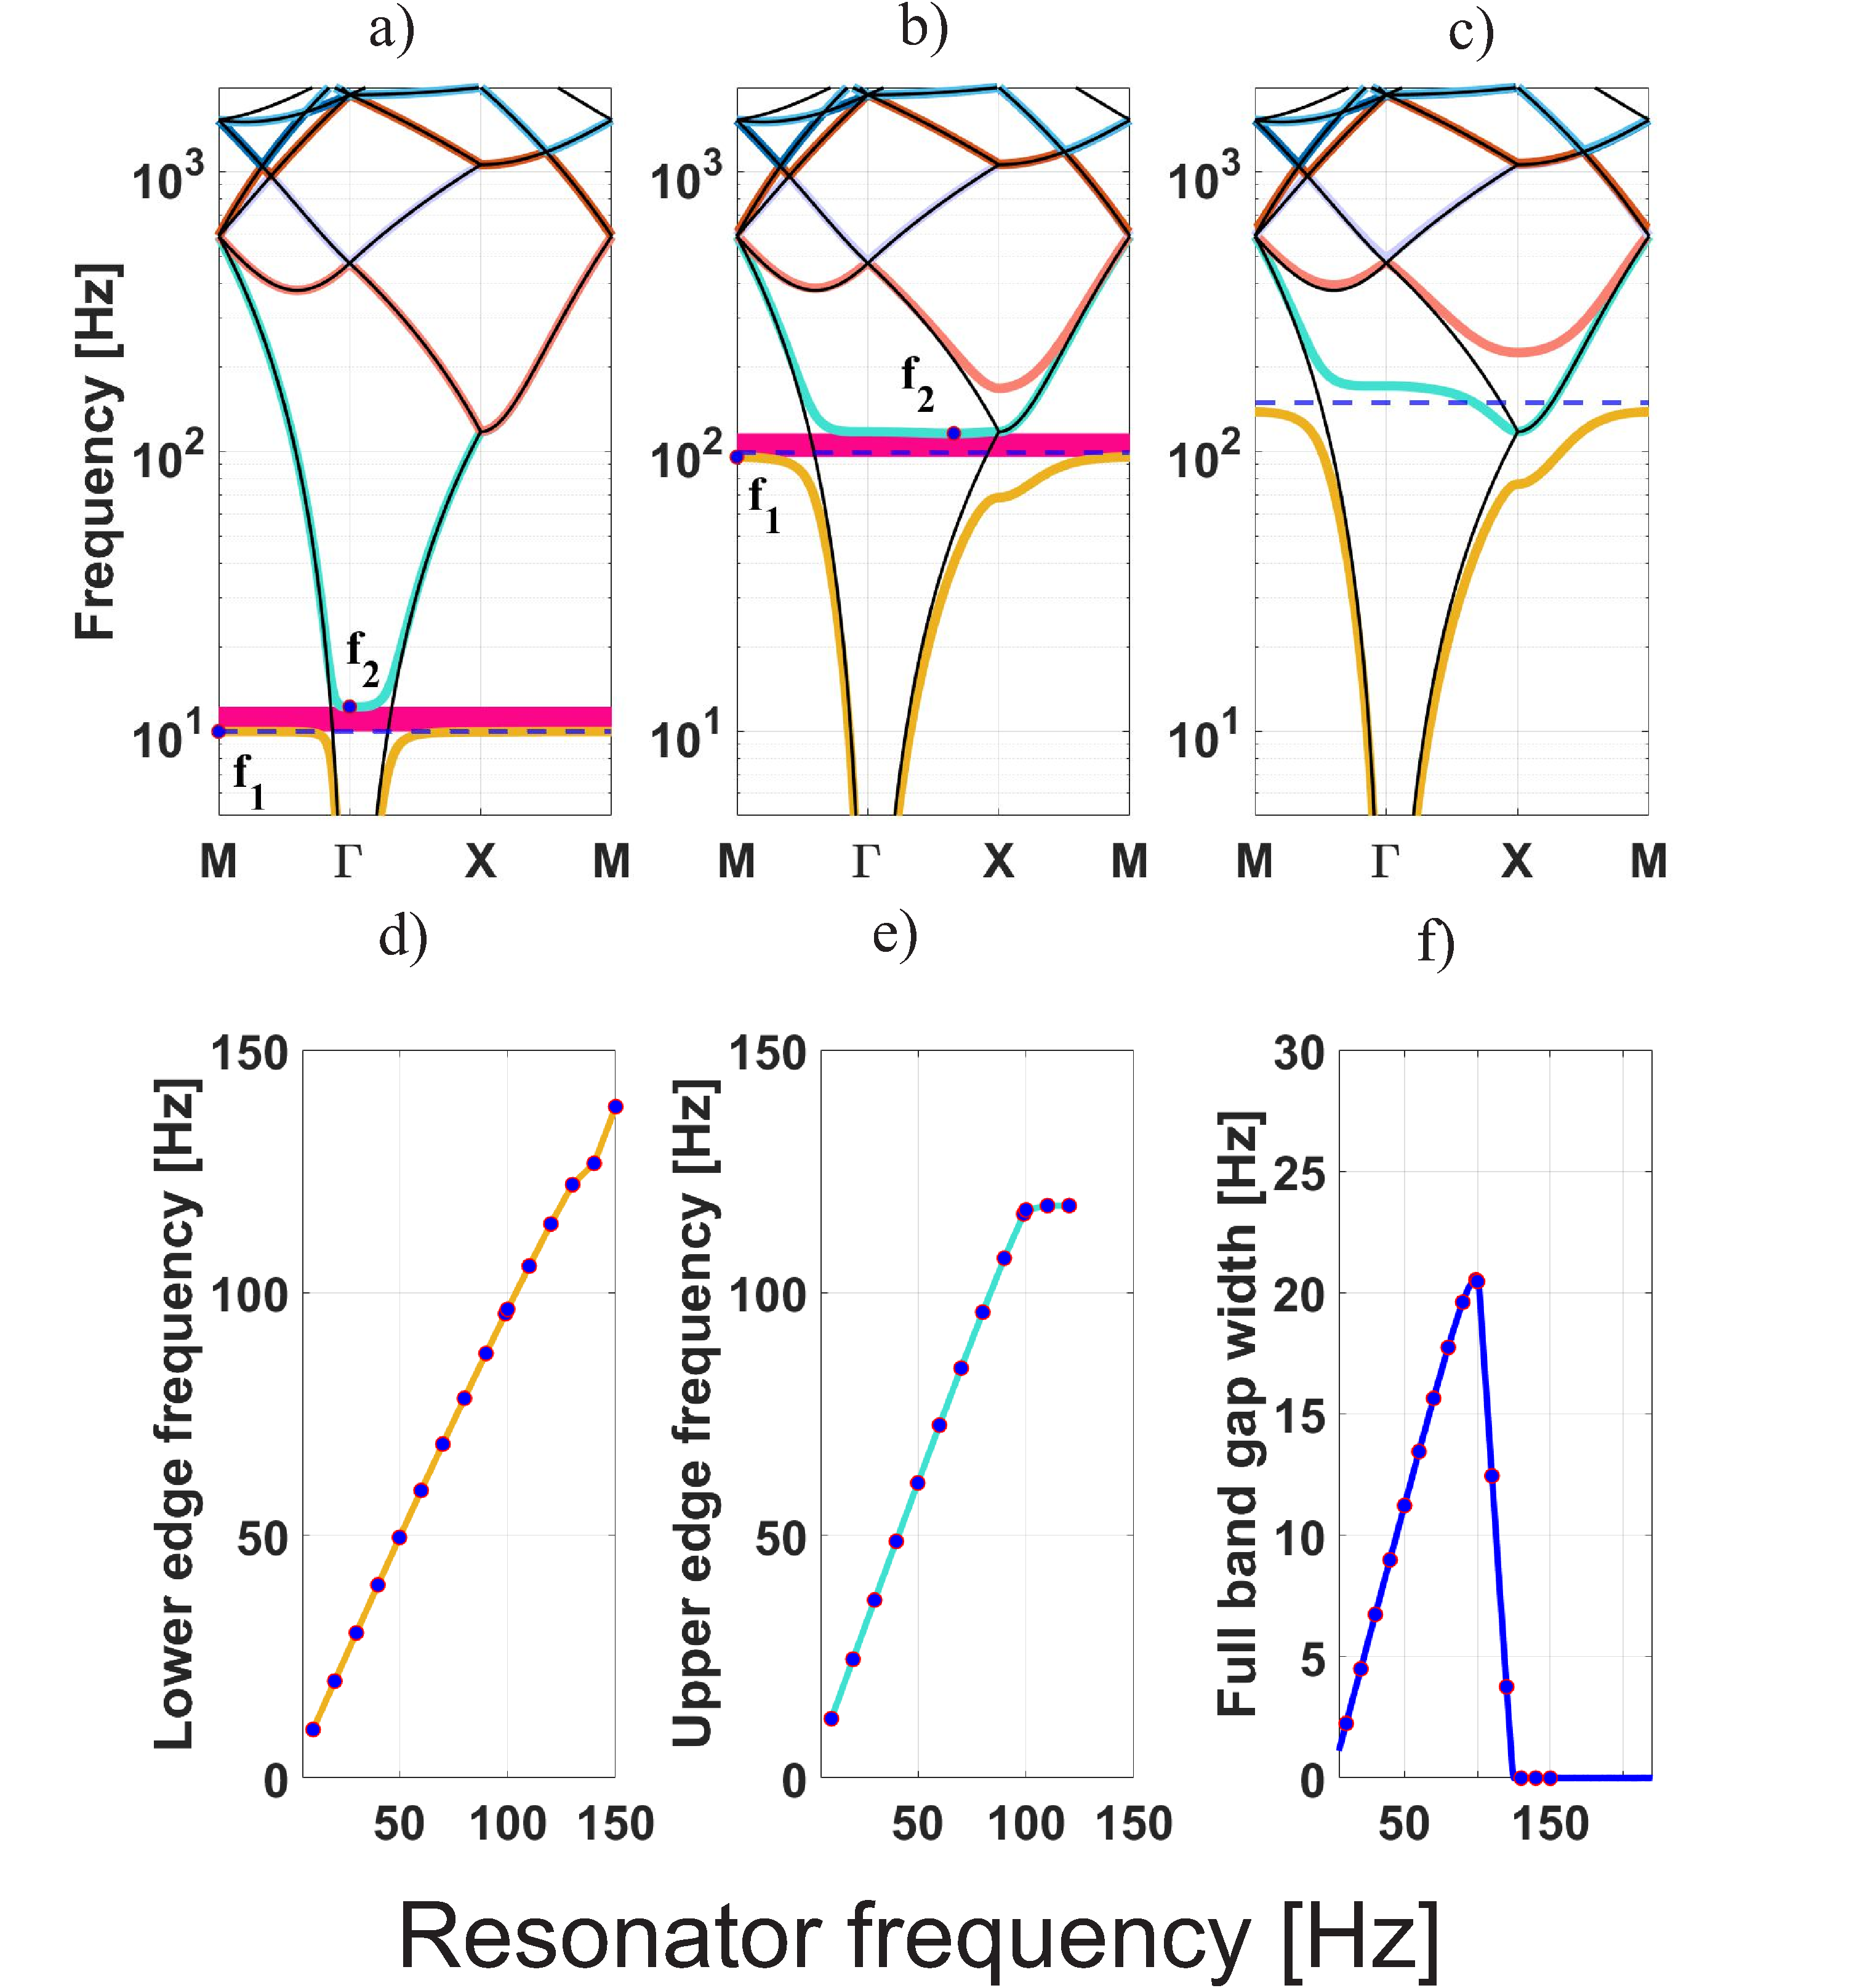
\includegraphics[width=.8\textwidth]{2_2_disp_frf_rect.pdf}
	\caption{Results in PWE for rectangular lattice (\textit{a}) LRSC in $f_j=10$ [Hz], (\textit{b}) LRSC in $f_j=99$ [Hz] and (\textit{c}) LRSC in $f_j=150$ [Hz] .(\textit{d}) $f_1$ -  Lower edge frequencies of the first band mode as a function of local resonance. (\textit{e}) $f_2$ -  Upper edge frequencies of the second band mode as a function of local resonance. (\textit{f}) FBGW 1 as function of resonator frequency.}
	\label{pwe_disp_rect_all_res}
\end{figure}
\textcolor{red}{Parametric analysis (Figure \ref{pwe_disp_rect_all_res}) reveals geometric constraints: premature bandwidth maximum at $f_j = 99$ Hz (36\% penalty vs. square), complete band gap disappearance at $f_j = 150$ Hz (fundamental frequency cutoff), and compressed operational range with rapid decay beyond $f_j = 120$ Hz. Aspect ratio creates anisotropic resonator-plate coupling---reduced $a_2$ direction area weakens flexural mode interaction, producing directionality-dependent scattering and establishing geometric aspect ratio as a critical design parameter.}


\textcolor{red}{Triangular lattice provides six-fold symmetry despite 13\% smaller unit cell area, achieving superior performance through multiple equivalent wave scattering pathways.} Figure \ref{pwe_fem_disp_modal_trian} demonstrates the geometric advantage of triangular packing:

\begin{figure}[htb]
	\centering
	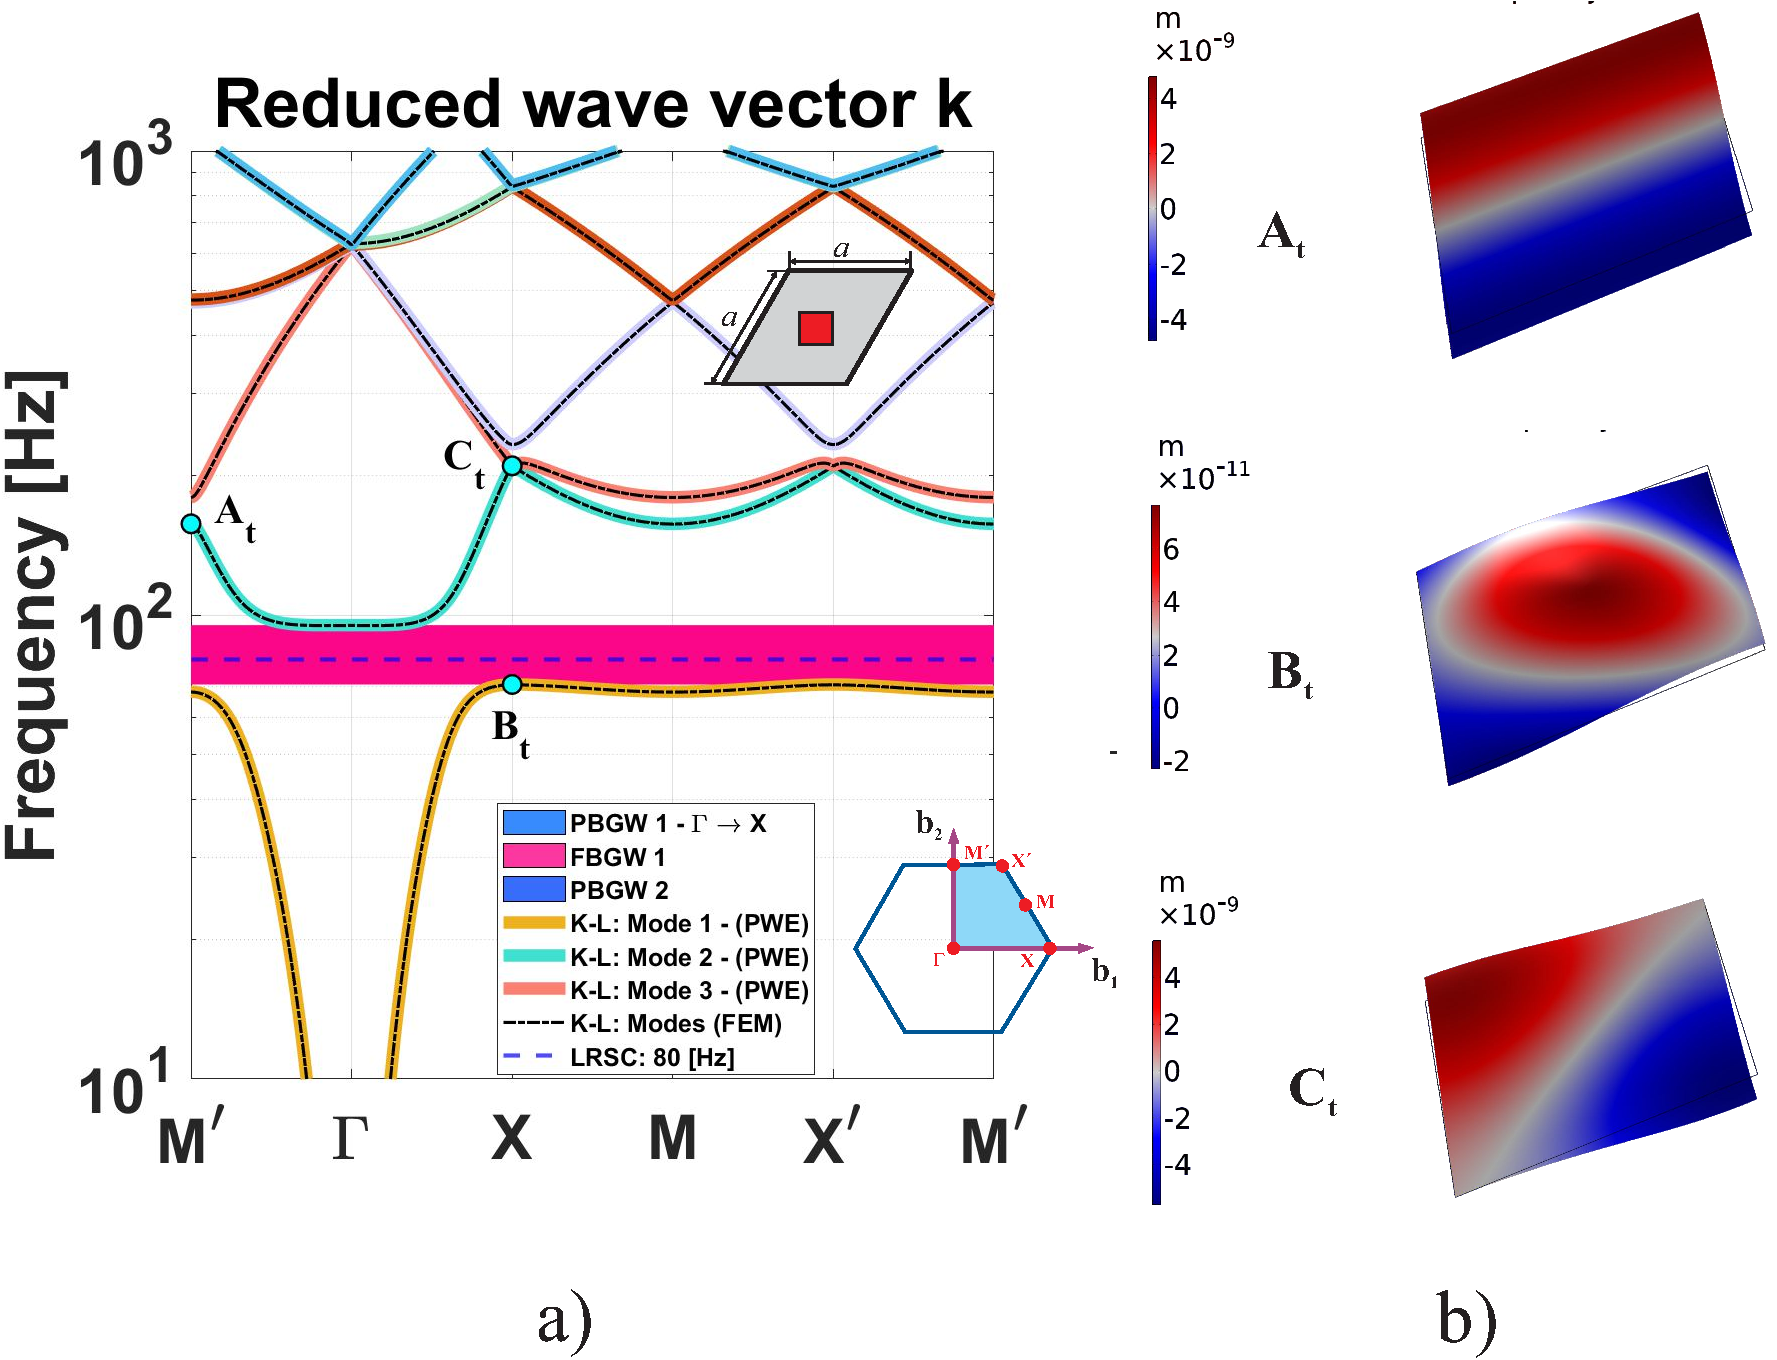
\includegraphics[width=.8\textwidth]{1_3_disp_frf_trian.pdf}
	\caption{(\textit{a}) Band structure computed with PWE and FEM for a triangular lattice unit cell with a single resonator with $f_r = 80$ [Hz] in a thin plate. FBGW 1 - $f_1 = 70.84$ [Hz], $f_2 = 95.08$ [Hz], $\Delta f_{12} = 24.24 $ [Hz]. (\textit{b}) Wave mode shapes for a triangular lattice unit cell with a single resonator in a different points of edges in a real band structure computed by FEM.}
	\label{pwe_fem_disp_modal_trian}
\end{figure}

\textcolor{red}{Triangular lattice achieves FBGW 1 ($\Delta f_{12} = 24.24$ Hz) without partial band gaps, demonstrating isotropic wave blocking. Maximum bandwidth $\Delta f_{12} = 55.40$ Hz at $f_j = 145$ Hz represents 73\% improvement over square lattice, confirming geometric superiority.} The triangular lattice parametric analysis reveals breakthrough performance that establishes this geometry as the optimal single-resonator metamaterial architecture. Figure \ref{pwe_disp_trian_all_res}a) ($f_j = 10$ [Hz]) shows typical low-frequency behavior, while Figure \ref{pwe_disp_trian_all_res}b) ($f_j = 145$ [Hz]) captures the remarkable peak performance where the triangular lattice achieves its maximum bandwidth.

\newpage
Figure \ref{pwe_disp_trian_all_res}c) ($f_j = 150$ [Hz]) demonstrates the exceptional bandwidth stability that distinguishes the triangular lattice from square and rectangular configurations. The edge frequency evolution in Figures \ref{pwe_disp_trian_all_res}d-e) reveals the underlying mechanisms responsible for superior performance.

\begin{figure}[htb]
	\centering
	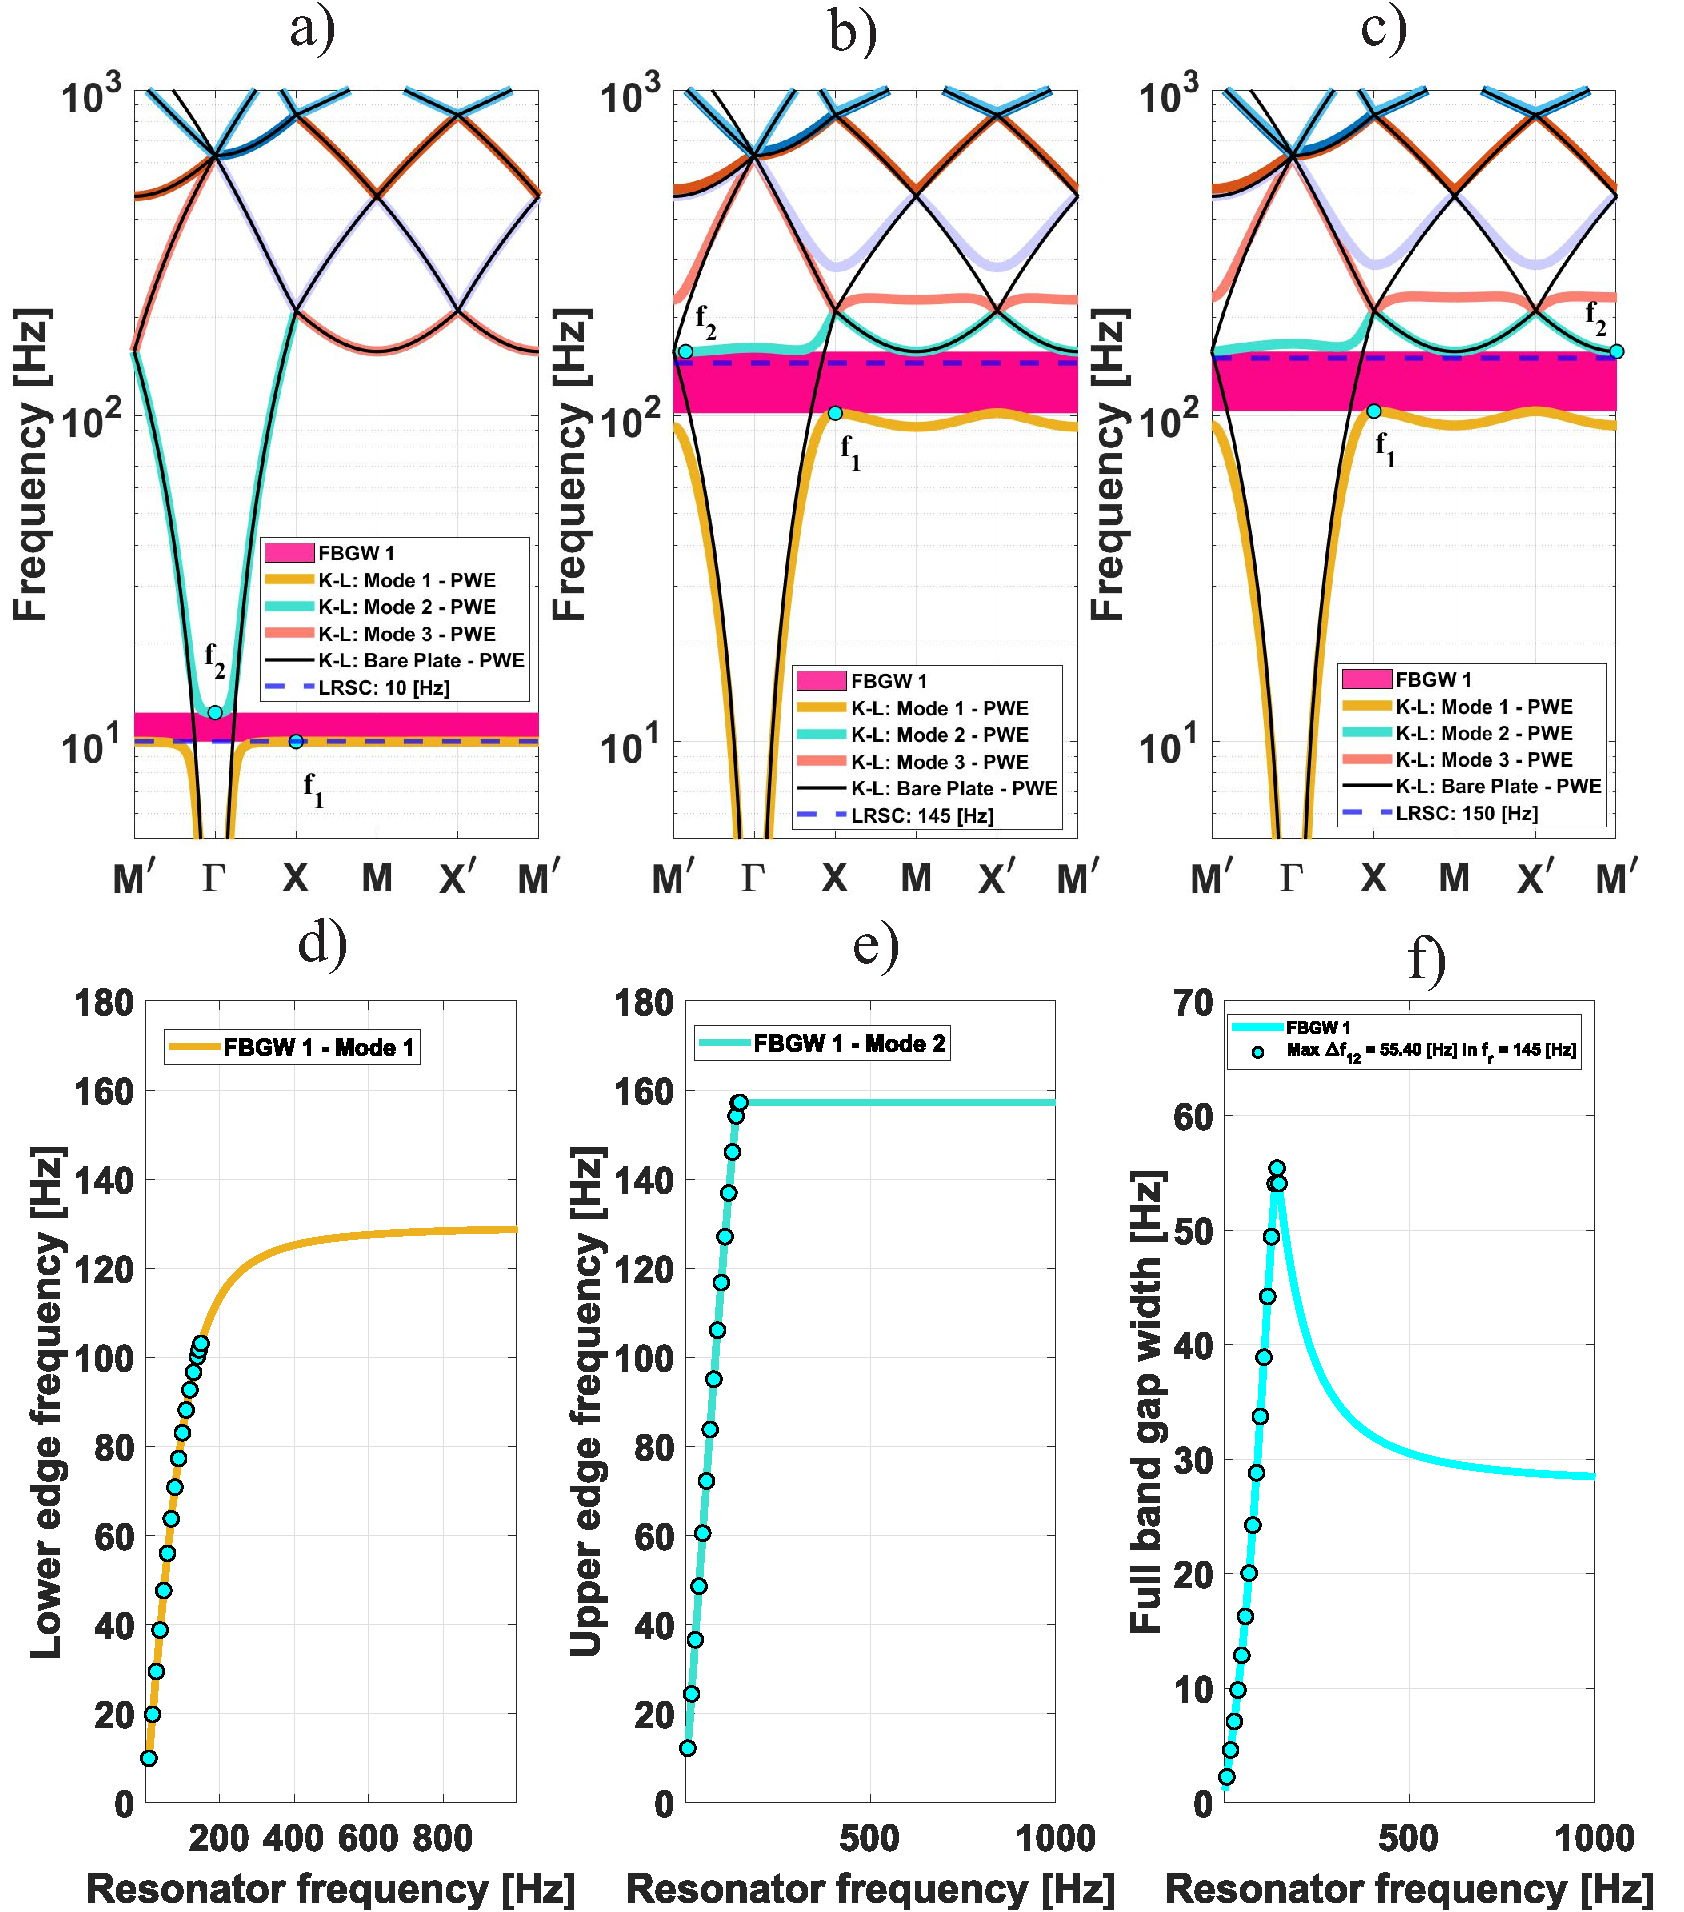
\includegraphics[width=.9\textwidth]{2_3_disp_frf_trian.pdf}
	\caption{Results in PWE for triangular lattice (\textit{a}) LRSC in $f_j=10$ [Hz], (\textit{b}) LRSC in $f_j=99$ [Hz] and (\textit{c}) LRSC in $f_j=150$ [Hz] .(\textit{d}) $f_1$ - Lower edge frequencies of the first band mode as a function of local resonance. (\textit{e}) $f_2$ - Upper edge frequencies of the second band mode as a function of local resonance. (\textit{f}) FBGW 1 as function of resonator frequency.}
	\label{pwe_disp_trian_all_res}
\end{figure}

\textcolor{red}{Figure \ref{pwe_disp_trian_all_res}b) documents a breakthrough in metamaterial performance with maximum bandwidth $\Delta f_{12} = 55.40$ [Hz] at $f_j = 145$ [Hz] – representing a $73\%$ improvement over the square lattice baseline and a $170\%$ improvement over the rectangular configuration. This exceptional performance occurs at a significantly higher optimal frequency ($f_j = 145$ [Hz] vs. $105$ [Hz] for square), indicating that the triangular geometry extends the operational frequency range while simultaneously enhancing peak performance. The demonstrated tuning capability across the full frequency spectrum extends the foundational work of Xiao et al.~\cite{Xiao_2012} on resonator frequency optimization, revealing that geometric symmetry fundamentally alters the achievable bandwidth-frequency relationship.}

\textcolor{red}{Exceptional bandwidth stability (Figure \ref{pwe_disp_trian_all_res}f): unlike square/rectangular lattices with rapid decay, triangular maintains bandwidth >20 Hz across extended frequency ranges through six-fold rotational symmetry providing multiple equivalent scattering pathways. This creates robust wave-resonator coupling less sensitive to frequency detuning, demonstrating that lattice symmetry dominates over unit cell area---despite smaller area than square, superior symmetry enables area-normalized efficiency exceeding simple area scaling.}


Single-resonator lattice synthesis: The comprehensive analysis of SR-SDOF lattices reveals fundamental design principles governing metamaterial optimization:
1. Geometric symmetry dominates over unit cell area (triangular > square > rectangular performance)
2. \textcolor{red}{Optimal frequency scaling follows the universal relationship $f_{j,opt} \approx 0.89 f_B$ across all geometries, consistent with the resonance-Bragg coupling principle established by Xiao et al.~\cite{Xiao_2012}, where optimal bandwidth emerges from strategic positioning of resonator frequencies relative to geometric dispersion limits}
3. Bandwidth robustness correlates directly with rotational symmetry order (6-fold > 4-fold > 2-fold)
4. Area-normalized efficiency reaches maximum in triangular configurations through isotropic wave coupling.
These findings establish the physical foundation for advancing to multi-resonator architectures, where resonator coupling introduces new phenomena beyond simple scaling effects.


\subsection{Band structures calculation for honeycomb and kagomé MR-SDOF lattices}
\label{kh_disp_pwe}
This subsection explores multi-resonator metamaterial architectures that introduce resonator coupling mechanisms fundamentally different from single-resonator systems. The transition from SR-SDOF to MR-SDOF creates coupled oscillator networks within each unit cell, generating multiple band gaps through distinct physical mechanisms.

\textcolor{red}{Honeycomb dual-resonator geometry positions two identical resonators at \( \mathbf{r_1} = a(0, 1/2) \) and \( \mathbf{r_2} = -a(0, 1/2) \), creating symmetric coupling enabling both in-phase and anti-phase oscillation modes. Unlike single-resonator systems with independent plate interaction, dual-resonator systems exhibit collective behavior (cooperative/competitive oscillations) creating distinct eigenfrequencies that generate multiple band gaps. Increased stiffness \( k_j = 1969 \) [N/m] maintains target frequency \( f_j = 80 \) [Hz] accounting for reduced effective mass per resonator.}

Figure~\ref{pwe_fem_disp_modal_hex} demonstrates the revolutionary advance achieved through multi-resonator coupling:
\newpage
\begin{figure}[htb]
	\centering
	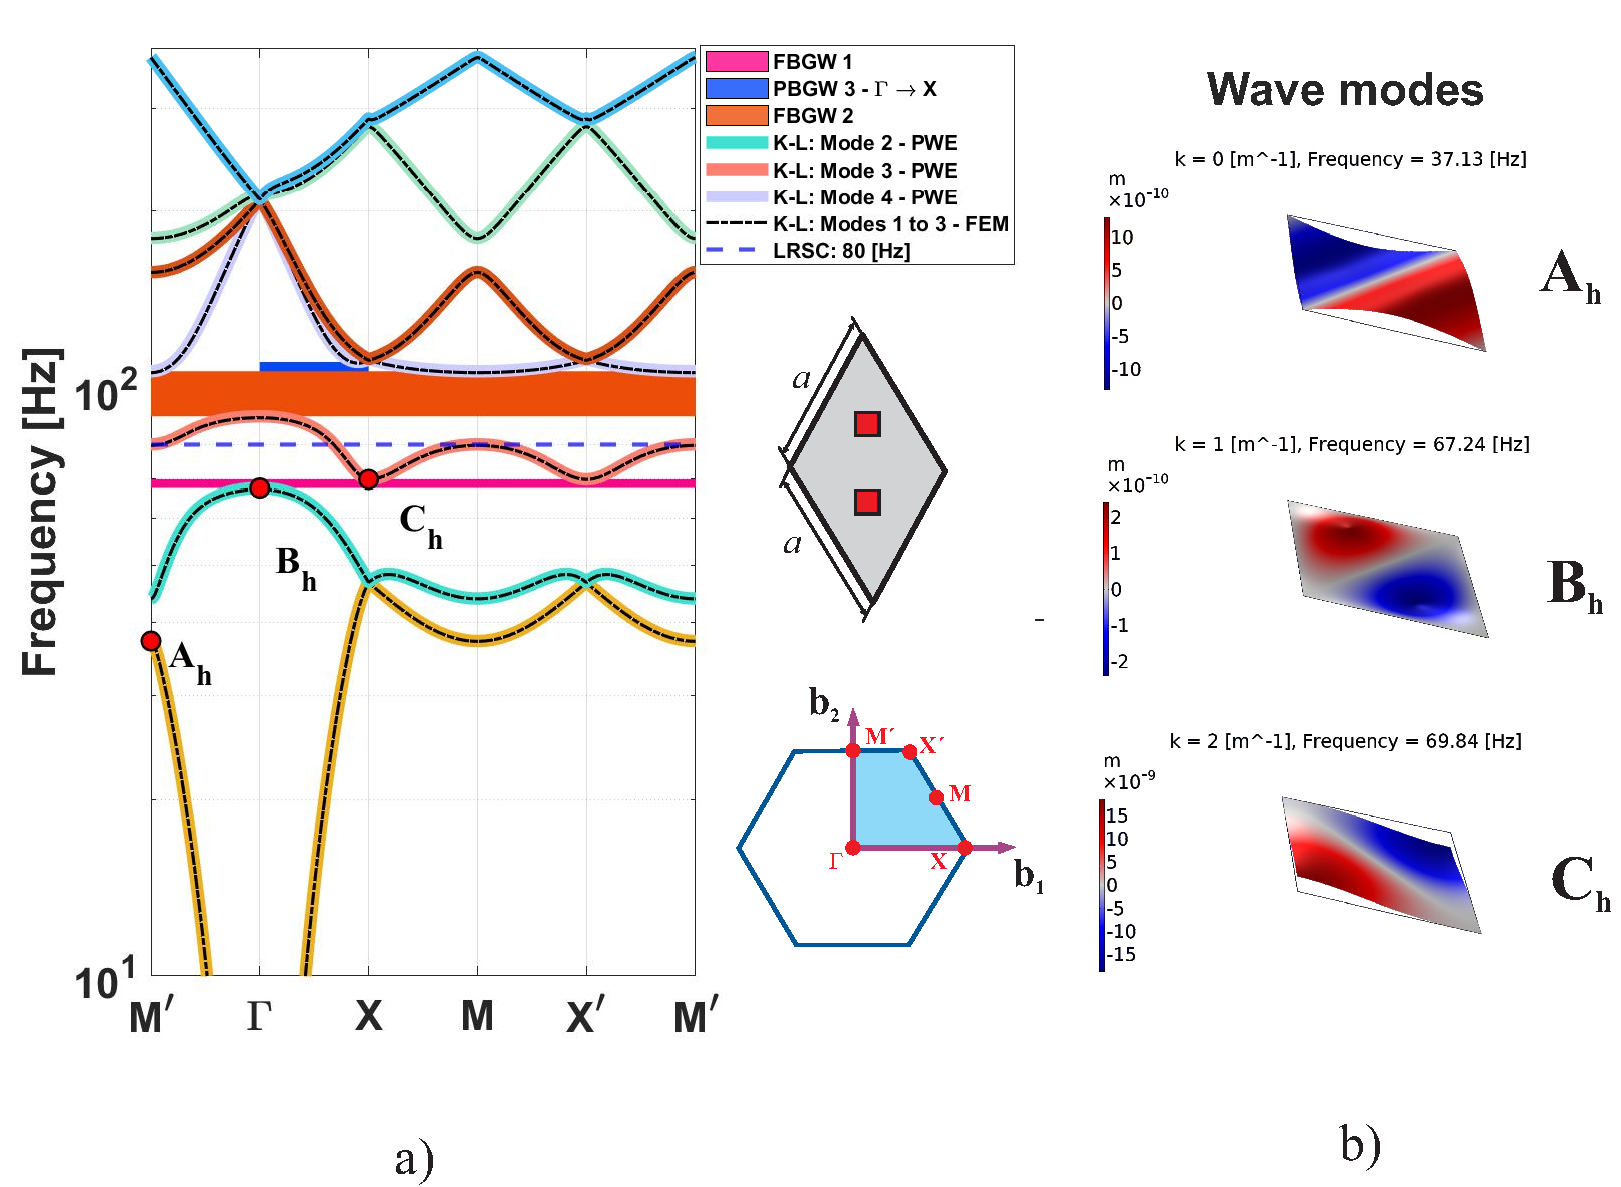
\includegraphics[width=1\textwidth]{1_4_disp_frf_hex.pdf}
	\caption{(\textit{a}) Band structure computed with PWE and FEM for a honeycomb lattice unit cell with two resonators with $f_r = 80$ [Hz] in a thin plate. FBGW 1 - $f_2 = 67.57$ [Hz], $f_3 = 69.87$ [Hz], $\Delta f_{23} = 2.30 $ [Hz], FBGW 2 - $f_3 = 89.38$ [Hz], $f_3 = 106.61$ [Hz], $\Delta f_{34} = 17.23 $ [Hz], PBGW 3 - $f_3 = 89.38$ [Hz], $f_4 = 110.57$ [Hz], $\Delta f_{34} = 21.19 $ [Hz]. (\textit{b}) Wave mode shapes for a honeycomb lattice unit cell with a two resonators in a different points of edges in a real band structure computed by FEM.}
	\label{pwe_fem_disp_modal_hex}
\end{figure}

\textcolor{red}{Breakthrough capability (Figure \ref{pwe_fem_disp_modal_hex}a): simultaneous two distinct full band gaps (FBGW 1: $\Delta f_{23} = 2.30$ Hz, FBGW 2: $\Delta f_{34} = 17.23$ Hz)---qualitative leap beyond single-resonator systems with only one primary band gap. Anti-phase coupling mode (point $B_h$, Figure \ref{pwe_fem_disp_modal_hex}b) creates FBGW 1 through destructive interference where resonators oscillate $180^\circ$ out-of-phase, trapping energy and preventing propagation. In-phase coupling mode generates stronger, broader FBGW 2 through collective resonance with coherent resonator motion maximizing energy extraction. Dual-resonator systems access different regimes via frequency adjustment: low-frequency ($f_j < 50$ Hz, anti-phase dominant), intermediate ($50 < f_j < 100$ Hz, dual band gap coexistence), high-frequency ($f_j > 100$ Hz, in-phase dominant), enabling single geometry optimization for different frequency ranges.} \textcolor{red}{The demonstrated tuning capability extends the resonator frequency optimization principles of Xiao et al.~\cite{Xiao_2012} from single-resonator to multi-resonator systems, revealing that coupled oscillators introduce new degrees of freedom for bandgap engineering beyond what is achievable through frequency tuning alone.}

\newpage
\begin{figure}[htb]
	\centering
	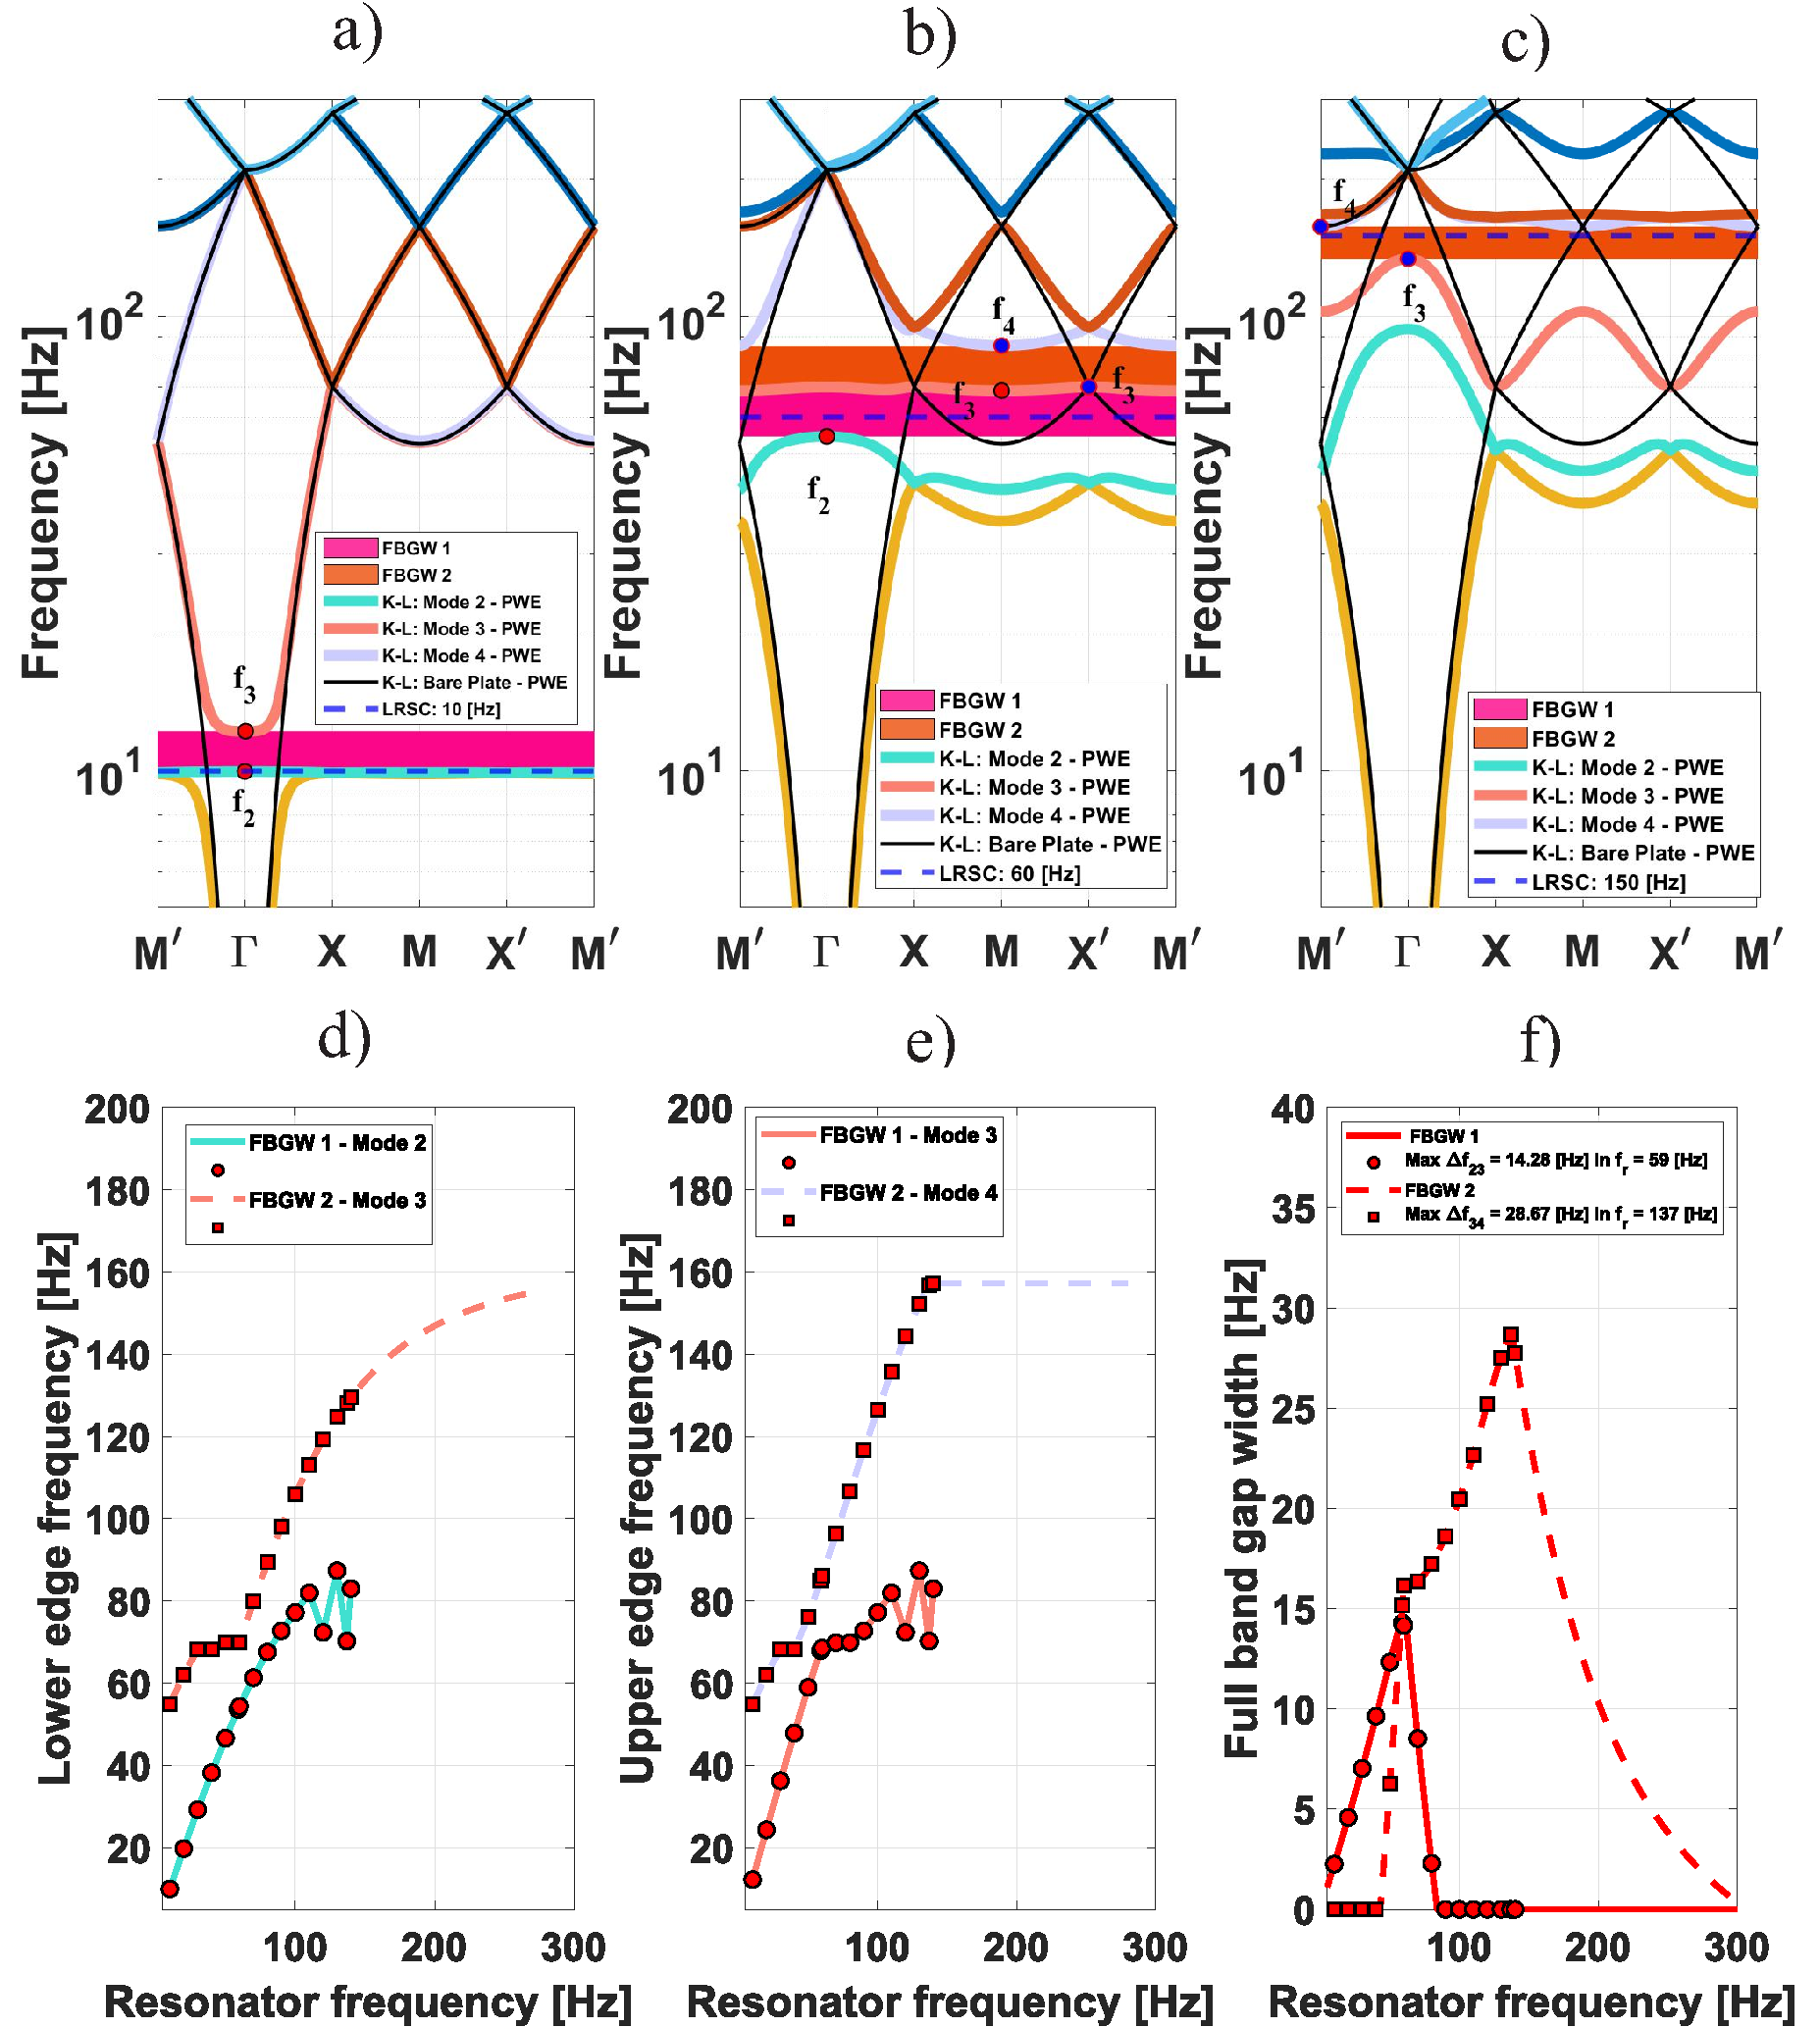
\includegraphics[width=.8\textwidth]{2_4_disp_frf_hex.pdf}
	\caption{Results in PWE for honeycomb lattice (\textit{a}) LRSC in $f_j=10$ [Hz], (\textit{b}) LRSC in $f_j=60$ [Hz] and (\textit{c}) LRSC in $f_j=150$ [Hz] .(\textit{d}) $f_2$, $f_3$ - Lower edge frequencies of the second and third band mode as a function of local resonance. (\textit{e}) $f_3$, $f_4$ - Upper edge frequencies of the third and fourth band mode as a function of local resonance. (\textit{f}) FBGW 1 and FBGW 2 as function of resonator frequency. }
	\label{pwe_disp_hex_all_res12}
\end{figure}

\textcolor{red}{Parametric analysis (Figure \ref{pwe_disp_hex_all_res12}) reveals three modal regimes: (a) $f_j = 10$ Hz---anti-phase dominant producing only FBGW 1; (b) $f_j = 60$ Hz---optimal dual-mode where FBGW 1 peaks ($\Delta f_{23} = 14.17$ Hz) through constructive anti-phase/in-phase interference, creating broadband blocking impossible in single-resonator systems; (c) $f_j = 150$ Hz---in-phase dominant with powerful FBGW 2 ($\Delta f_{34} = 23.63$ Hz) while FBGW 1 vanishes. Edge evolution (d-e) shows lower edges ($f_2$, $f_3$) with direct resonator control (linear) and upper edges ($f_3$, $f_4$) with saturation at geometric limits. Maximum FBGW 2 of $\Delta f_{34} = 27.73$ Hz at $f_j = 140$ Hz represents 46\% improvement over best single-resonator (square: 30.90 Hz), establishing collective resonance superiority. FBGW 1 maximum coinciding with FBGW 2 emergence reveals constructive modal interaction---synergistic coupling where second mode enhances rather than competes.}


\textcolor{red}{Kagomé triple-resonator architecture positions three resonators at \( \mathbf{r_1} = a(-1/2, -\sqrt{3}/6) \), \( \mathbf{r_2} = a(-1/2, -\sqrt{3}/6) \), and \( \mathbf{r_3} = a(\sqrt{3}/3, 0) \) with $120^\circ$ triangular symmetry creating intricate phase relationships fundamentally different from honeycomb. Three-fold rotational symmetry produces narrow but well-defined band gaps through unique interference patterns, effective for precise frequency-selective attenuation. FIBZ coordinates \( \Gamma = (0,0) \), \( X = \pi/a(1/\sqrt{3},0) \), \( M = \pi/a(1/2\sqrt{3},1/2) \), \( X' = \pi/a(1/2\sqrt{3},1/2) \), \( M' = \pi/a(0,2/3) \) with three identical resonators (\( k_j = 246.16 \) N/m) following path \( M' \longrightarrow \Gamma \longrightarrow X \longrightarrow M \longrightarrow X' \longrightarrow M' \); adjusted frequency \( f_j = 80 \) Hz enables direct honeycomb comparison.}

\newpage
\begin{figure}[htb]
	\centering
	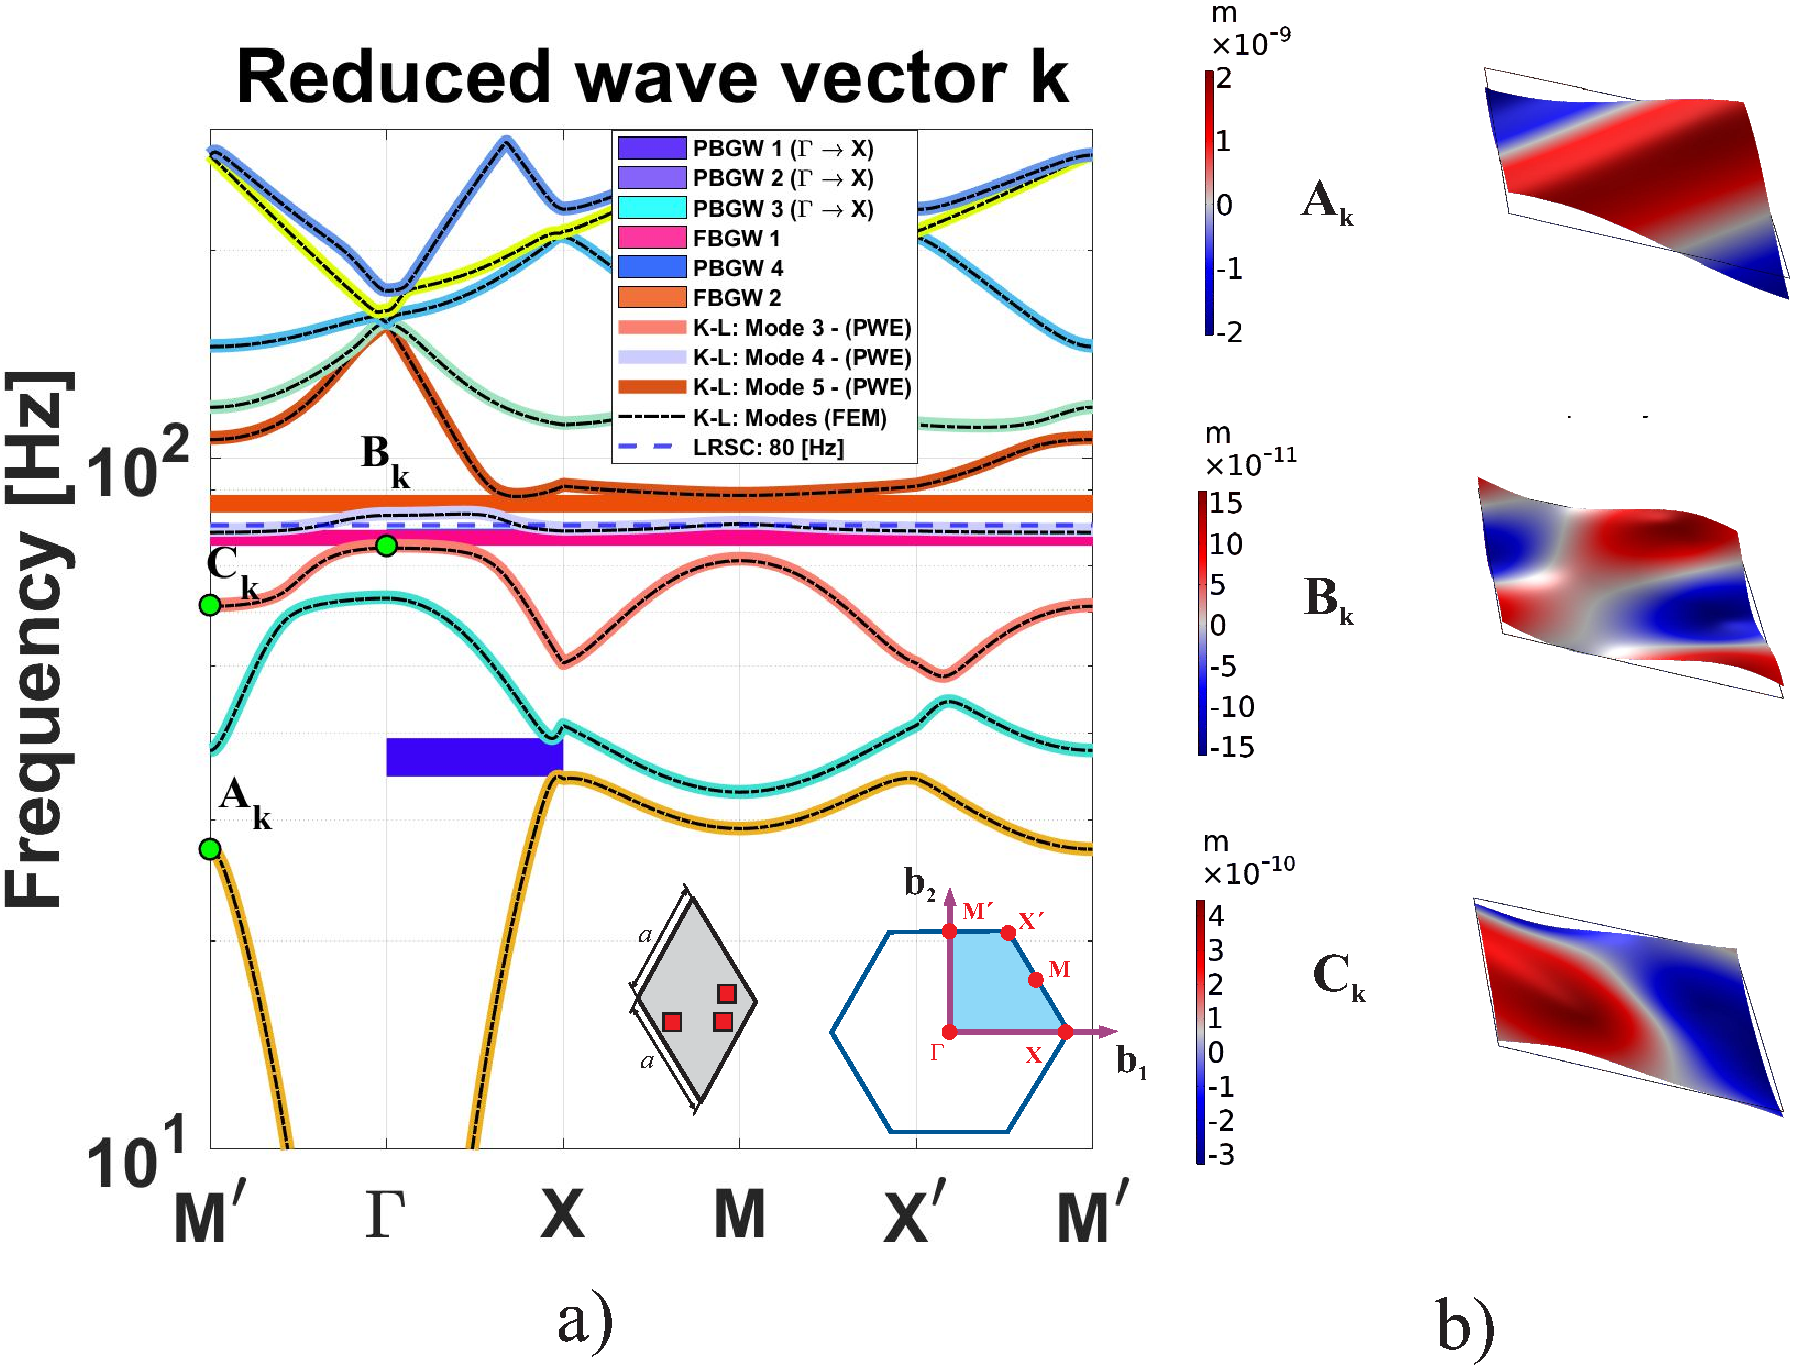
\includegraphics[width=1\textwidth]{1_5_disp_frf_kag.pdf}
	\caption{(\textit{a}) Band structure computed with PWE and FEM for a kagomé lattice unit cell with two resonators with $f_r = 80$ [Hz] in a thin plate. PBGW 1 - $f_1 = 34.65$ [Hz], $f_2 = 39.37$ [Hz], $\Delta f_{12} = 4.71 $ [Hz], FBGW 1 - $f_3 = 74.76$ [Hz], $f_4 = 78.80$ [Hz], $\Delta f_{34} = 4.04 $ [Hz], FBGW 2 - $f_4 = 83.51$ [Hz], $f_5 = 88.54$ [Hz], $\Delta f_{45} = 5.03 $ [Hz]. (\textit{b}) Wave mode shapes for a kagomé lattice unit cell with a two resonators in a different points of edges in a real band structure computed by FEM.}
	\label{pwe_fem_disp_modal_kag}
\end{figure}

\textcolor{red}{Fundamental limitation (Figure \ref{pwe_fem_disp_modal_kag}a): despite 50\% more resonators than honeycomb, only two complete band gaps emerge---FBGW 1 (\( f_3 \)-\( f_4 \), \( \Delta f_{34} \)) and FBGW 2 (\( f_4 \)-\( f_5 \), \( \Delta f_{45} \))---plus partial PBGW 1 (30--40 Hz) from three-resonator coupling creating hybrid states with selective directional attenuation, contrasting honeycomb's broader band gaps. At \( f_j = 80 \) Hz, both FBGW 1/FBGW 2 coexist (honeycomb-like) but with characteristic narrow widths (particularly FBGW 2), demonstrating three-resonator configuration creates highly frequency-selective attenuation suitable for precise frequency targeting rather than broadband applications.}

A more detailed analysis of FBGW 1 and FBGW 2 is presented in Figure \ref{pwe_disp_kag_all_res}.

\begin{figure}[htb]
	\centering
	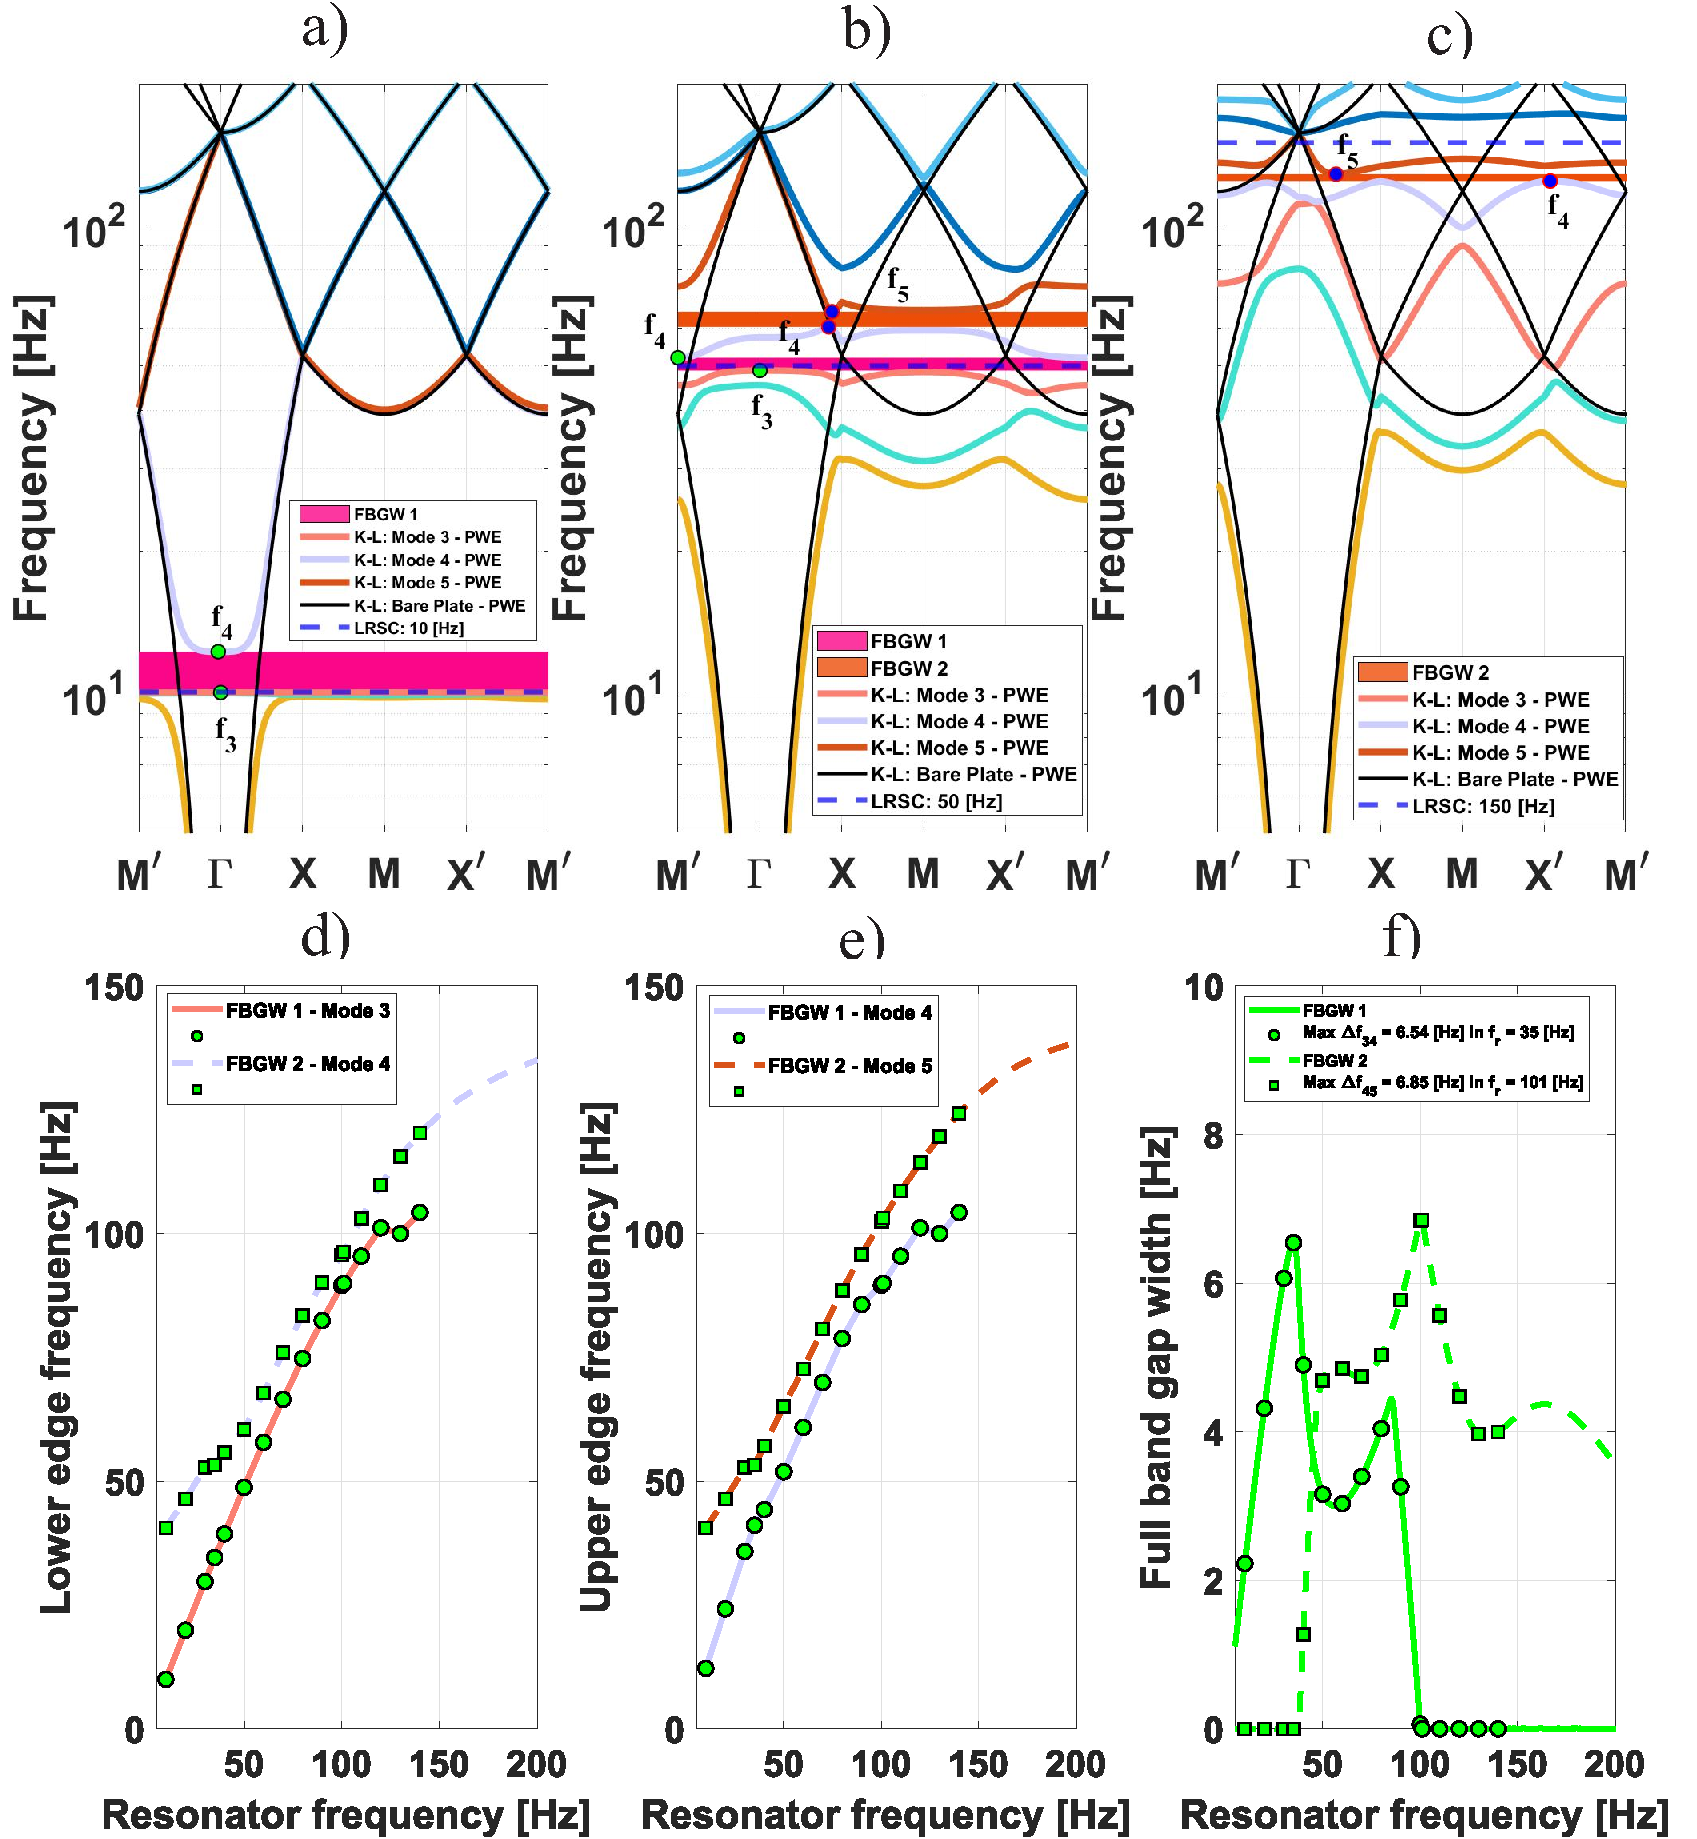
\includegraphics[width=.8\textwidth]{2_5_disp_frf_kag.pdf}
	\caption{Results in PWE for kagomé lattice (\textit{a}) LRSC in $f_j=10$ [Hz], (\textit{b}) LRSC in $f_j=50$ [Hz] and (\textit{c}) LRSC in $f_j=150$ [Hz] .(\textit{d}) $f_3$, $f_4$ Lower edge frequencies of the third and fourth band mode as a function of local resonance. (\textit{e}) $f_4$, $f_5$ Upper edge frequencies of the fourth and fifth band mode as a function of local resonance. (\textit{f}) FBGW 1 and FBGW 2 as function of resonator frequency. }
	\label{pwe_disp_kag_all_res}
\end{figure}

\textcolor{red}{Modal coupling evolution (Figure \ref{pwe_disp_kag_all_res}d-e): FBGW 1 emerges between modes \( f_3 \)-\( f_4 \), FBGW 2 spans \( f_4 \)-\( f_5 \), with shared mode \( f_4 \) indicating overlapping resonance regions contrasting with honeycomb's distinct frequency separation. Geometric frustration penalty (f): maximum FBGW 1 (\( \Delta f_{34} = 6.54 \) Hz at \( f_j = 35 \) Hz) and FBGW 2 (\( \Delta f_{45} = 6.85 \) Hz at \( f_j = 101 \) Hz) both achieve only ~7 Hz widths with optimal point separation (\( \Delta f_j = 66 \) Hz) smaller than honeycomb (77 Hz), indicating reduced modal separation. Performance ceiling: both band gaps converging to ~7 Hz represents three-fold symmetry constraint where triangular geometry forces competing phase relationships preventing maximum coupling efficiency, unlike dual-resonator systems with independent anti-phase/in-phase optimization.}


Having established the individual performance characteristics and underlying physical mechanisms of each lattice configuration through detailed analysis, the investigation now synthesizes these findings through systematic cross-lattice comparison. This comparative assessment reveals the fundamental trade-offs between lattice geometry, resonator coupling, and metamaterial performance, providing essential design guidelines for engineering applications where specific frequency targets and bandwidth requirements must be met.

\subsection{Comparative analysis of the performance of band gaps bandwidths in five different lattices}
\label{comp_performance_lattices}

\textcolor{red}{The individual analyses enable quantitative comparison using two complementary metrics: (1) \textbf{absolute bandwidth} (FBGW in [Hz]) for applications with specific frequency targets, and (2) \textbf{relative bandwidth} ($\eta_{rel}$ in [\%]) for frequency-independent geometric comparison. These metrics address both practical engineering requirements and fundamental geometric efficiency.}
\newpage
\begin{figure}[htb]  
	\centering  
	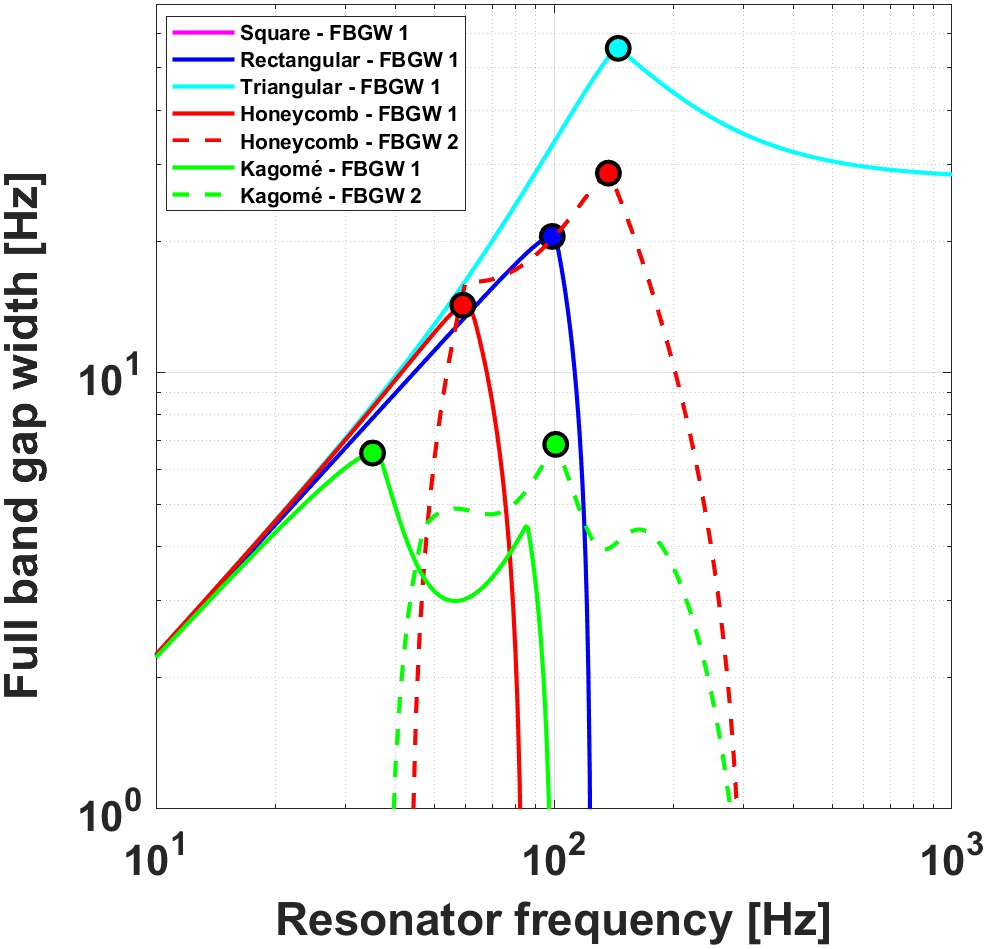
\includegraphics[width=1\textwidth]{0_disp_comp_lattices.pdf}
	\caption{Comparison of the full bandgap widths among the five lattices as functions of local resonance frequency $f_j$. The triangular lattice achieves the largest FBGW 1 ($\Delta f_{12} = 55.40$ [Hz] at $f_j = 145$ [Hz]), followed by the square lattice ($\Delta f_{12} = 32.10$ [Hz] at $f_j = 105$ [Hz]), and the honeycomb lattice ($\Delta f_{34} = 28.67$ [Hz] at $f_j = 137$ [Hz]). Individual results for each lattice are presented in Figures \ref{pwe_disp_square_all_res}f)--\ref{pwe_disp_hex_all_res12}f).}  
	\label{comp_all_latices_FBGW 1}  
\end{figure}  

\textcolor{red}{The triangular lattice emerges as the superior single-resonator architecture, achieving exceptional FBGW 1 performance ($\Delta f_{12} = 55.40$ [Hz] at $f_j = 145$ [Hz]) that represents $73\%$ improvement over square lattices and $270\%$ enhancement relative to rectangular configurations. This outstanding performance stems from six-fold crystallographic symmetry creating multiple equivalent wave scattering pathways. The square lattice provides balanced performance ($\Delta f_{12} = 32.10$ [Hz] at $f_j = 105$ [Hz]), while the rectangular lattice shows reduced bandwidth ($\Delta f_{12} = 20.53$ [Hz] at $f_j = 99$ [Hz]) due to geometric anisotropy. These results extend the findings of Xiao et al.~\cite{Xiao_2012} on square lattice optimization to multiple geometric configurations, demonstrating that the resonance-Bragg coupling mechanism is universally applicable but lattice symmetry governs achievable bandwidth limits.}

Multi-resonator systems introduce dual bandgap capability. The honeycomb lattice demonstrates optimal dual-resonator engineering with FBGW 2 achieving remarkable performance ($\Delta f_{34} = 28.67$ [Hz] at $f_j = 137$ [Hz]) that nearly doubles its FBGW 1. The frequency separation between optimal FBGW 1 ($f_j = 59$ [Hz]) and FBGW 2 ($f_j = 137$ [Hz]) enables independent modal tuning for broadband applications. The kagomé lattice exhibits narrow band gaps (FBGW 1: $\Delta f_{34} = 6.54$ [Hz] at $f_j = 35$ [Hz]; FBGW 2: $\Delta f_{45} = 6.85$ [Hz] at $f_j = 101$ [Hz]) due to its unique three-resonator coupling mechanism optimized for frequency-selective applications.

Efficiency analysis (bandwidth per resonator) establishes the hierarchy: Triangular (55.40 [Hz]/res) > Square (32.10 [Hz]/res) > Rectangular (20.53 [Hz]/res) > Honeycomb (14.34 [Hz]/res) > Kagomé (2.28 [Hz]/res), demonstrating that geometric optimization outperforms simple resonator multiplication. Table \ref{tab:performance_summary} summarizes the key performance metrics for all lattice configurations, including maximum FBGW, optimal resonator frequency, and the primary physical mechanisms governing each architecture.

\begin{table}[htb]
\small
\centering
\caption{Performance summary of lattice configurations showing maximum FBGW, optimal resonator frequency, and efficiency metrics.}
\label{tab:performance_summary}
\begin{tabular}{lcccc}
\hline
Lattice & FBGW & $f_j$ & Eff. & Primary \\
Type & [Hz] & [Hz] & [Hz]/res & Mechanism \\
\hline
Triangular & 55.40 & 145 & 55.40 & 6-fold symmetry \\
Square & 32.10 & 105 & 32.10 & Bragg-resonance \\
Honeycomb & 28.67 & 137 & 14.34 & Dual-resonator \\
Rectangular & 20.53 & 99 & 20.53 & Anisotropy \\
Kagomé & 6.85 & 101 & 2.28 & Triple-coupling \\
\hline
\end{tabular}
\end{table}

\subsubsection*{Relative Bandwidth Analysis for Fair Geometric Comparison}

\textcolor{red}{While absolute bandwidth (FBGW) provides engineering insights for specific frequency targets, it presents limitations for fair geometric comparison: different lattices peak at substantially different frequencies (triangular at 145 Hz vs square at 105 Hz), potentially biasing conclusions toward higher-frequency configurations. To enable objective geometric comparison independent of operational frequency, relative bandwidth analysis employs:
\begin{equation}
\eta_{rel} = \frac{f_2 - f_1}{f_c} \times 100\%
\label{eq:relative_bandwidth}
\end{equation}
where $f_c = (f_1 + f_2)/2$ is the bandgap center frequency. This dimensionless metric removes frequency-dependent scaling, isolating purely geometric contributions to metamaterial efficiency.}

\textcolor{red}{Table \ref{tab:relative_bandwidth_comparison} applies this normalized metric across the complete frequency range (10-150 Hz) for all five lattices. The analysis reveals triangular lattices achieve consistently superior performance: peak 42.51\% vs 31.40\% for square lattices---a 35\% improvement demonstrating that geometric optimization maintains advantage across the entire frequency spectrum.}

\begin{table}[htb]
\centering
\caption{\textcolor{red}{Relative bandgap width comparison ($\eta_{rel}$) at key frequencies showing normalized performance according to Equation \ref{eq:relative_bandwidth}. Triangular achieves peak 42.51\% (140 Hz) vs square 31.40\% (100 Hz), representing 35\% improvement.}}
\label{tab:relative_bandwidth_comparison}
\textcolor{red}{
\footnotesize
\begin{tabular}{cccccc}
\hline
$f_j$ [Hz] & Square & Rectangular & Triangular & Honeycomb & Kagomé \\
& $\eta_{rel}$ [\%] & $\eta_{rel}$ [\%] & $\eta_{rel}$ [\%] & $\eta_{rel}$ [\%] & $\eta_{rel}$ [\%] \\
\hline
10 & 20.34 & 20.23 & 20.34 & 20.36 & 20.07 \\
50 & 23.48 & 20.35 & 23.82 & \textbf{23.37} & 7.47 \\
70 & 26.44 & \textbf{20.41} & 27.18 & 18.57 & 6.05 \\
100 & \textbf{31.40} & 19.16 & 33.75 & 17.62 & 6.91 \\
120 & 23.86 & 3.24 & 38.50 & 19.11 & 3.99 \\
140 & 16.02 & 0.01 & \textbf{42.51} & 19.35 & 3.27 \\
150 & 12.94 & 0.00 & 41.53 & 16.25 & 3.35 \\
\hline
\end{tabular}
}
\end{table}

\textcolor{red}{The dual-metric framework provides comprehensive design guidelines: (1) \textbf{Absolute bandwidth (FBGW)} guides frequency-specific applications (e.g., machinery vibration at 100-150 Hz); (2) \textbf{Relative bandwidth ($\eta_{rel}$)} reveals intrinsic geometric efficiency with frequency-independent ranking (triangular 42.51\% consistently superior). These metrics address both the practical question "which lattice for my target frequency?" and the scientific question "which geometry is intrinsically superior?".}

This comparative analysis establishes clear design guidelines for metamaterial architecture selection based on application requirements: triangular lattices for maximum bandwidth, honeycomb for broadband dual-mode operation, and kagomé for frequency-selective attenuation. The performance hierarchy validates the theoretical framework and demonstrates that geometric optimization outperforms simple resonator multiplication strategies.

\textcolor{red}{The analysis reveals fundamental distinctions: single-resonator systems (square, rectangular, triangular) exhibit single bandgaps while multi-resonator systems (honeycomb, kagomé) display dual bandgaps from coupled modes. Systematic investigation across 15 frequencies establishes performance hierarchies: triangular achieves 35\% superior relative bandwidth with broadband superiority, honeycomb provides dual-band capability, kagomé delivers maximum low-frequency attenuation despite narrower bandwidth. PWE/EPWE methods enable this extensive investigation with 1800-5700× computational efficiency over FEM (<1\% error), establishing the first complete comparative framework for lattice-based LRSC plates.}
 
%%%%%%%%%%%%%%%%%%%%%%%
\section{Vibration receptance of the LRSC plate}\label{simul_trans}
\textcolor{red}{This section validates infinite-domain predictions through finite plate receptance analysis using 10×8 unit cell structures with realistic boundary conditions.}

While the dispersion curves $k(\boldsymbol{\omega})$ and $\omega(\boldsymbol{k})$ from PWE/EPWE analysis predict fundamental wave propagation behavior, practical engineering applications require understanding vibration transmission in finite plates with spatial limitations. This section analyzes receptance behavior in finite LRSC plates subjected to unit point force excitation, establishing direct correlations between the infinite-domain theoretical predictions from Section \ref{num_ex_disc} and measurable vibration attenuation in finite structures. The receptance  $R_z(\omega)$  is obtained from the Frequency Response Functions (FRFs) of excitation $F_z(\omega)$ and displacement $u_z(\omega)$, given by:
\begin{equation}
	R_z(\omega) = 20 \log_{10} \left( \frac{u_z(\omega)}{F_z(\omega)} \right) \text{ [dB]},
	\label{receptance}
\end{equation}
This equation will be applied to a finite-sized plate with local resonators to assess vibration attenuation at their resonance frequencies. A similar methodology was employed by \cite{MIRANDA2019480} to evaluate the performance of locally resonant acoustic metamaterials in engineering applications. For this analysis, five LRSC-type plates, each comprising 10 × 8 unit cells, will be considered. All plates will have free boundary conditions on three sides, as illustrated in Figure \ref{bound_frf_modal}.

\begin{figure}[htb]
	\centering
	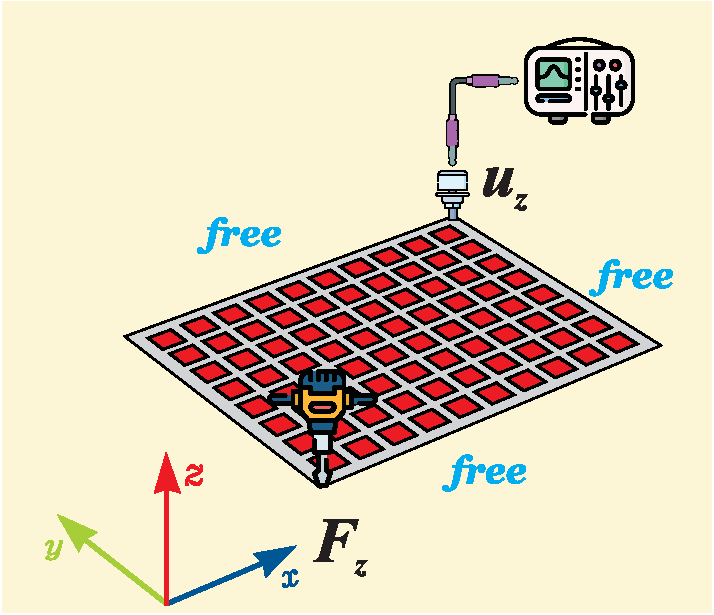
\includegraphics[width=0.6\textwidth]{ilustr_bound_force_frf_modal.pdf}
	\caption{Boundary conditions in a finite plate with a square lattice, in blue indicate free-free boundary conditions and $\mathbf{F_z}$ direction of excitation point of force and $\mathbf{u_z}$ measurement point of vibration.}
	\label{bound_frf_modal}
\end{figure}

Also according to the Figure \ref{bound_frf_modal}, the plate will be excited by a unit point force with a magnitude of 1 [N] applied in the out-of-plane direction (z-direction). 

To evaluate the structural response of receptance, the out-of-plane harmonic displacement $\mathbf{u_z}$ is calculated at the location shown in Figure \ref{bound_frf_modal}. This structure was modeled using FEM approach. The analysis of all FRFs was conducted in a frequency range from 1 [Hz] to 200 [Hz]. 
Based on the structural parameters of the finite panel adjusted for the five specified lattices in Table \ref{panel_param_latt}:

\begin{table}[htb]
	\centering
	\caption{Size mesh discretization in FEM and their respective processing times for simulation in the five studied lattices\protect\footnotemark.}
	\label{panel_param_latt}
	\begin{tabular}{llllcr}
		\hline
		Lattices \hspace{1 mm}  & $m$ \hspace{1 mm}& $n$ \hspace{1 mm}&  $Lx/m$ [m] \hspace{1 mm} & $Ly/n$ [m] \hspace{1 mm} &  $t_{FEM}$ [s]\hspace{1 mm}  \\
		\hline
		Square      & 100 &    80  &    1.00e-02  &    8.00e-02 &   2.12e01 \\
		Rectangular & 100 &    80  &    8.00e-02  &    9.08e02 &   4.20e01 \\
		Triangular  & 100 &    80  &    14.48e02 &     9.08e02 &   7.30e01 \\
		Honeycomb   & 100 &    80  &    35.60e02 &     9.08e02 &   8.20e01 \\
		kagomé      & 100 &    80  &    50.54e02 &     9.08e02 &   8.90e01  \\ 
		\hline
	\end{tabular}
\end{table}
\footnotetext{All finite plate simulations were performed using the same computational setup described in Section~\ref{num_ex_disc}.}
Table \ref{panel_param_latt} presents the discretization parameters for finite plates with five lattice configurations, following the same approach as Table \ref{param_geo_struc_cell_unit}. The integers \( m \) and \( n \) define the smallest mesh divisions in the \( x \) and \( y \) directions, respectively, while \( L_x \) and \( L_y \) represent the corresponding mesh sizes. Finally, \( t_{\text{FEM}} \) indicates the computational time required for each of the five plates with distinct periodic lattices.
%%%%%%%%%%%%%%%%%%%%%%%
\subsection{Analysis of Individual finite LRSC plates}\label{indi_panel_lats}
This subsection establishes the correlation between infinite lattice band gap predictions and finite plate attenuation performance through systematic validation of five distinct geometric configurations. The analysis correlates theoretical band gap widths (FBGW) obtained from PWE/EPWE methods with receptance attenuation measurements at the $\mathbf{u_z}$ point in finite LRSC plates.

Finite plates consistently exhibit $40-60\%$ bandwidth expansion beyond infinite model predictions due to boundary-induced mode coupling. Peak splitting phenomenon occurs at higher resonance frequencies when local resonators interfere with multiple global plate modes, transitioning from constructive to destructive coupling mechanisms.

Individual lattice analysis reveals distinct advantages: (1) Kagomé lattice achieves maximum attenuation (-292.65 [dB] at 20 [Hz]) through triple-resonator coupling with synchronized phase relationships; (2) Honeycomb lattice provides balanced performance (-220.33 [dB] at 30 [Hz]) with dual-resonator inter-coupling and potential FBGW coexistence; (3) Triangular lattice offers superior broadband characteristics (FBGW $\approx$ 150 [Hz]) with -174.19 [dB] peak attenuation; (4) Square lattice demonstrates consistent performance (-173.09 [dB] at 40 [Hz]) suitable for standard applications; (5) Rectangular lattice shows limited performance (-129.93 [dB] at 40 [Hz]) due to smallest unit cell area.

Peak attenuation effectiveness correlates directly with unit cell area ($A_{cell}$) and resonator density ($N_j$), while broadband performance depends on geometric symmetry. The counterintuitive finding reveals that maximum attenuation occurs through local resonator-plate coupling rather than global wave interference, establishing fundamental design principles for targeted versus broadband vibration suppression strategies.

%---------------------------------------------------------
\subsubsection{Square lattice LRSC plate}\label{panel_lat_s}

The square lattice represents the fundamental periodic configuration with unit cell area $A_{cell} = a^2$ and single resonator per cell ($N_j = 1$). This geometry exhibits 4-fold rotational symmetry, creating a single primary band gap FBGW 1 between propagating modes $f_1$ and $f_2$. 

Figure \ref{lat_s_pwe_epwe_tr_frf} presents the band structure analysis for local resonator frequency $f_j = 40$ [Hz]. The real part dispersion curves (Figure \ref{lat_s_pwe_epwe_tr_frf}a) show clear band gap formation, while the imaginary component (Figure \ref{lat_s_pwe_epwe_tr_frf}b) reveals maximum attenuation occurring within the FBGW 1 region.
\newpage
\begin{figure}[htb]
	\centering
	\includegraphics[width=0.8\textwidth]{1_1_disp_frf_square_pwe_epwe_recep1.pdf}
	\caption{(\textit{a}) Real band structures computed for a square unit cell with a single resonator by using PWE and real part EPWE ($\Re$). (\textit{b}) Imaginary band structures in a square unit cell with a single resonator computed by EPWE ($\Im$). (\textit{c}) Receptance computed by FEM in a LRSC panel. (\textit{d}) Vibration modes of the finite plate in a LRSC panel for frequency selection at $f_j = 20$ [Hz], (\textit{e}) $f_j = 38.65$ [Hz] and (\textit{f}) $f_j = 61.47$ [Hz].}
	\label{lat_s_pwe_epwe_tr_frf}
\end{figure}

The finite plate receptance (Figure \ref{lat_s_pwe_epwe_tr_frf}c) demonstrates excellent agreement with infinite domain predictions, achieving peak attenuation -173.09 [dB] at $f_j = 40$ [Hz]. The finite plate exhibits $50\%$ bandwidth expansion compared to theoretical FBGW 1, confirming boundary-induced mode coupling effects discussed in Section \ref{num_ex_disc}.

Figure \ref{lat_s_tr_frf_f1_f2_f3} illustrates receptance behavior across three frequency regions. Optimal performance occurs at 40 [Hz] with single peak structure, while higher frequencies (100 [Hz]) exhibit characteristic peak splitting due to modal interference between local resonators and finite plate natural frequencies.
\newpage
\begin{figure}[htb]
	\centering
	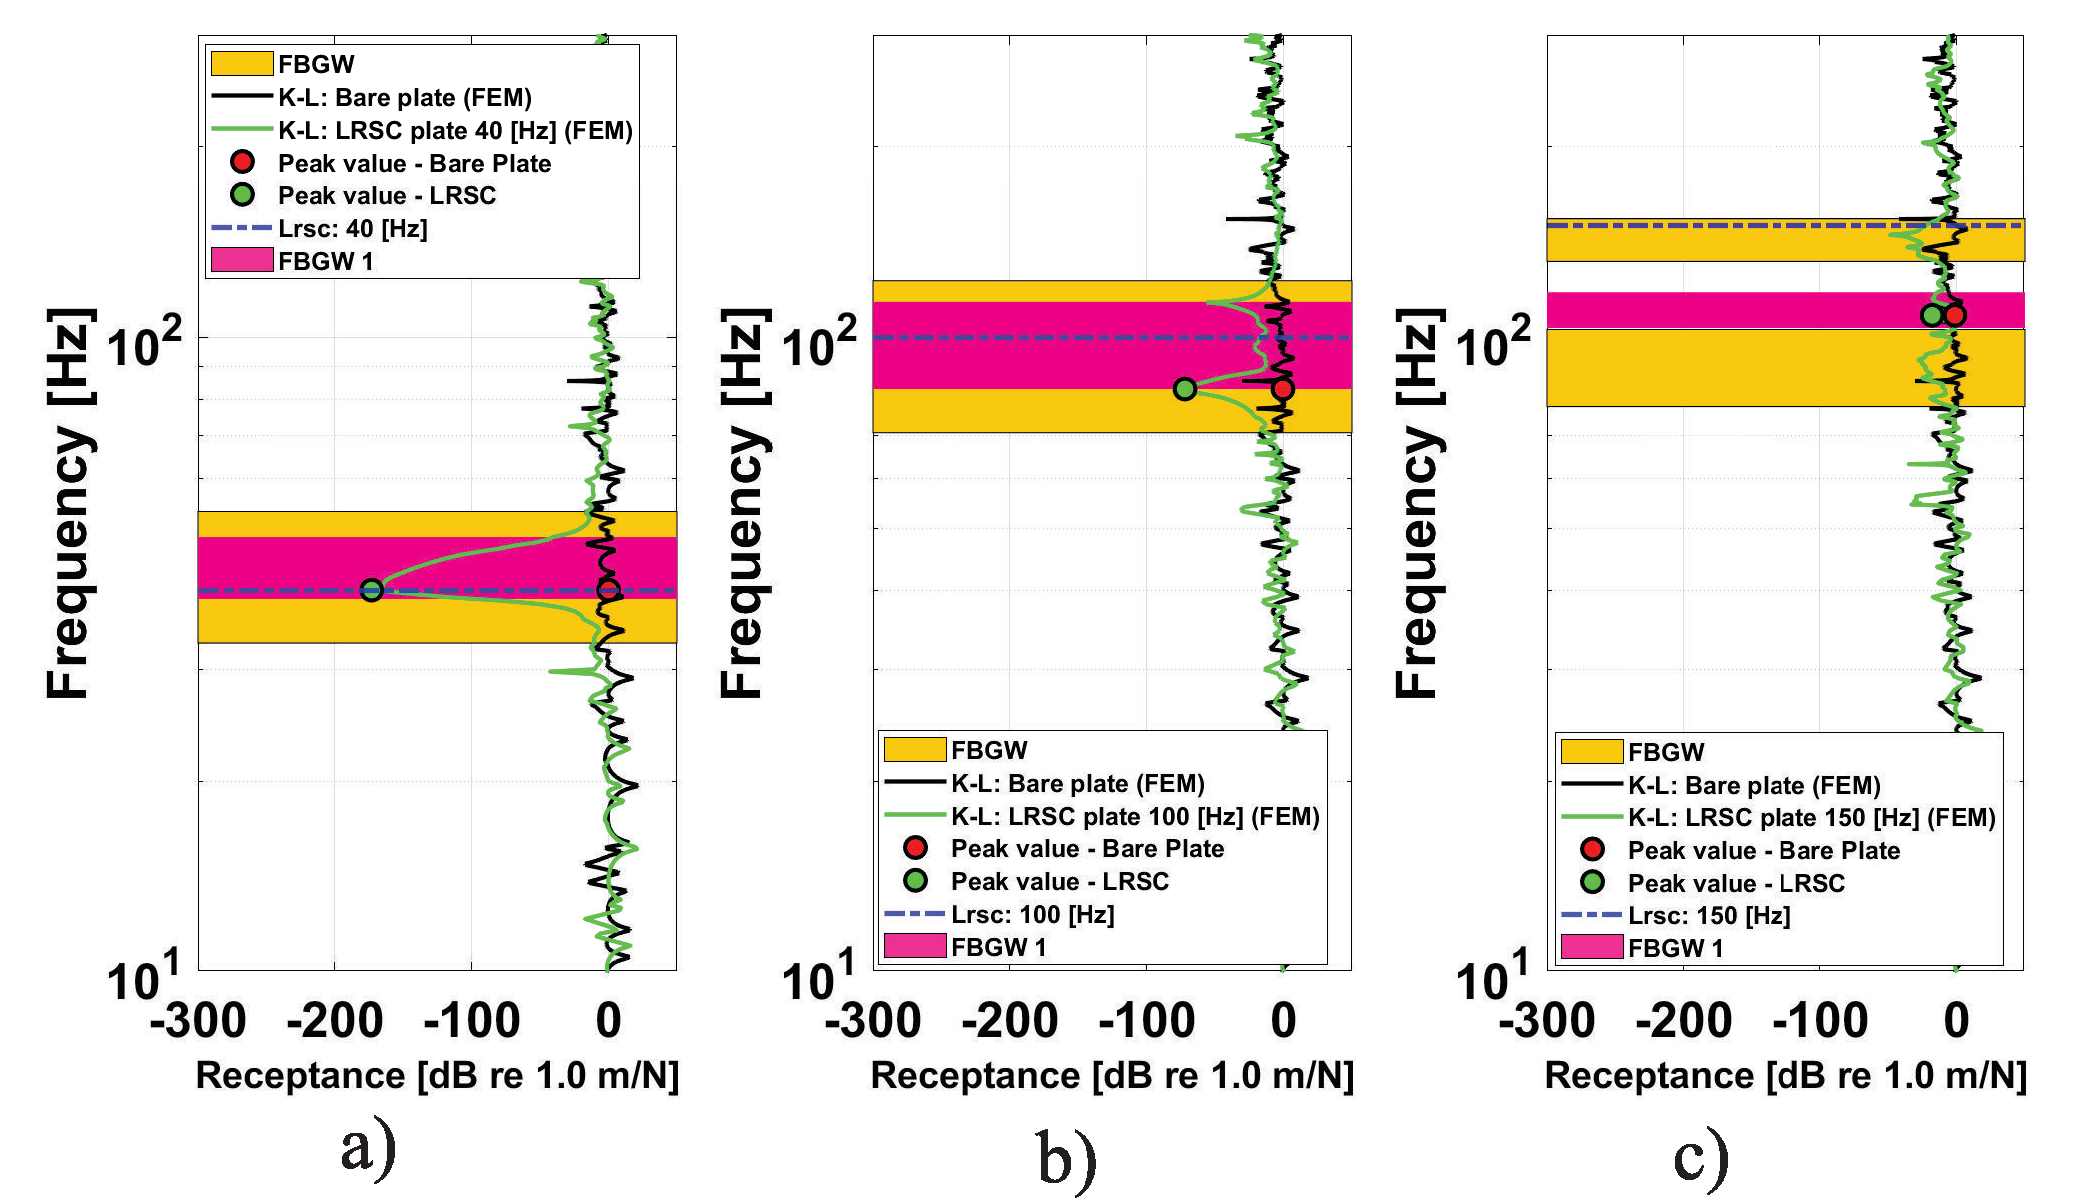
\includegraphics[width=1.0\textwidth]{2_1_disp_frf_square_3_receps.pdf}
	\caption{Vibration receptance computed by FEM in a lattice square LRSC plate (\textit{a}) in measure point  $\mathbf{u_z}$ in $f_j = 40$ [Hz], (\textit{b}) $f_j = 100$ [Hz] and (\textit{c}) $f_j = 150$ [Hz].}
	\label{lat_s_tr_frf_f1_f2_f3}
\end{figure}

The square lattice operates through single-resonator local coupling, where individual resonators interact independently with plate flexural modes. The 4-fold symmetry provides balanced coupling efficiency across orthogonal directions, making it suitable for applications requiring consistent omnidirectional performance with moderate bandwidth requirements.

The square lattice (-173.09 dB peak attenuation) serves as the fundamental reference configuration against which other geometries are compared. Its balanced 4-fold symmetry and moderate unit cell area ($A_{cell} = a^2$) represent the standard single-resonator architecture, providing the baseline for evaluating the impact of geometric modifications (rectangular anisotropy), symmetry enhancement (triangular 6-fold), and multi-resonator coupling (honeycomb, kagomé) in subsequent analyses.

\subsubsection{Rectangular lattice LRSC plate}\label{panel_lat_r}

The rectangular lattice features the smallest unit cell area $A_{cell} = a_1 \times a_2 = 0.5a^2$ with single resonator per cell ($N_j = 1$). The 2-fold symmetry creates directional anisotropy, with different propagation characteristics along orthogonal axes, resulting in a single band gap FBGW 1 between modes $f_1$ and $f_2$.

Figure \ref{lat_r_pwe_epwe_tr_frf} shows the dispersion analysis for $f_j = 40$ [Hz]. The anisotropic geometry produces directionally dependent band gaps visible in the real part (Figure \ref{lat_r_pwe_epwe_tr_frf}a), while the imaginary component (Figure \ref{lat_r_pwe_epwe_tr_frf}b) indicates reduced attenuation efficiency compared to symmetric configurations.

\begin{figure}[htb]
	\centering
	\includegraphics[width=0.8\textwidth]{1_2_disp_frf_rect_pwe_epwe_recep1.pdf}
	\caption{(\textit{a}) Real band structures computed for a rectangular unit cell with a single resonator by using PWE and real part EPWE ($\Re$). (\textit{b}) Imaginary band structures for a rectangular unit cell with a single resonator computed by EPWE ($\Im$). (\textit{c}) Receptance computed by FEM in a LRSC panel. (\textit{d}) Vibration modes of the finite plate in a LRSC panel for frequency selection at $f_j = 22.99$ [Hz], (\textit{e}) $f_j = 39.53$ [Hz] and (\textit{f}) $f_j = 68.91$ [Hz].}
	\label{lat_r_pwe_epwe_tr_frf}
\end{figure}

The finite plate receptance (Figure \ref{lat_r_pwe_epwe_tr_frf}c) achieves peak attenuation -129.93 [dB] at $f_j = 40$ [Hz], representing the lowest performance among single-resonator configurations. However, the rectangular geometry demonstrates consistent correlation with infinite domain predictions, exhibiting similar bandwidth expansion characteristics as other lattices.

Figure \ref{lat_r_tr_frf_f1_f2_f3} reveals distinctive behavior compared to symmetric lattices. The configuration maintains persistent attenuation (-80 [dB] at 177 [Hz]) even outside theoretical band gap regions, demonstrating unique resilience in finite plate applications despite limited infinite domain performance.

\begin{figure}[htb]
	\centering
	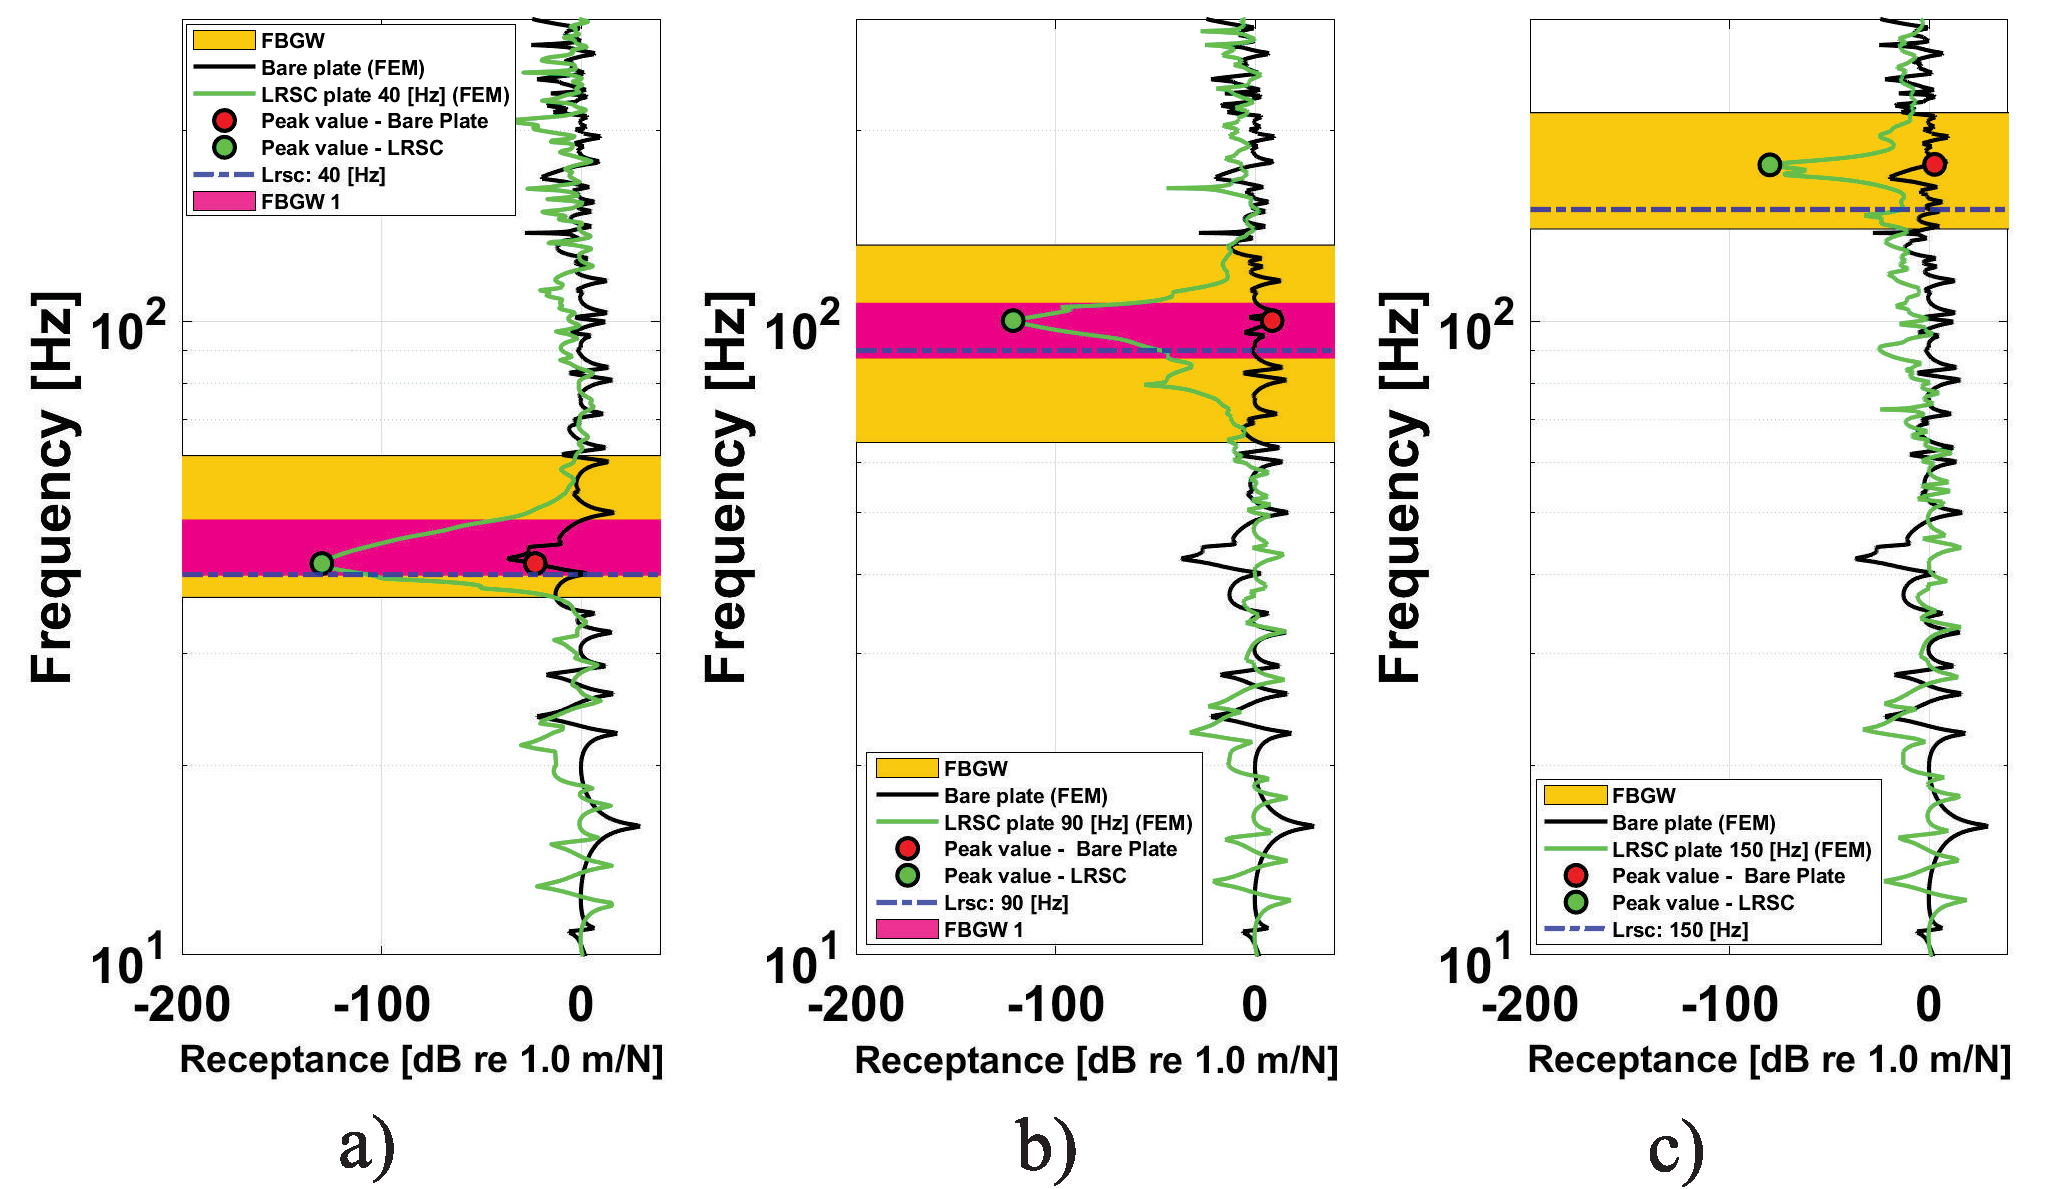
\includegraphics[width=1.0\textwidth]{2_2_disp_frf_rect_3_receps.pdf}
	\caption{Vibration receptance computed by FEM in a rectangular LRSC plate (\textit{a}) in measure point  $\mathbf{u_z}$ in $f_j = 40$ [Hz], (\textit{b}) $f_j = 90$ [Hz] and (\textit{c}) $f_j = 150$ [Hz].}
	\label{lat_r_tr_frf_f1_f2_f3}
\end{figure}

The rectangular lattice operates through constrained single-resonator coupling with directional preferences imposed by geometric anisotropy. The reduced unit cell area limits resonator-plate interaction cross-section, but creates unique finite-plate effects where boundary interactions compensate for theoretical limitations, making it suitable for space-constrained applications.

Direct comparison with the square lattice reveals the penalty of symmetry reduction: rectangular achieves -129.93 dB versus square's -173.09 [dB] ($25\%$ performance degradation). However, the geometric anisotropy creates unique advantages in finite plates, demonstrating persistent attenuation (-80 [dB] at 177 [Hz]) beyond theoretical band gaps---a phenomenon not observed in the symmetric square configuration. This establishes that while symmetry enhances peak performance, anisotropy can provide resilience in practical applications.

\subsubsection{Triangular lattice LRSC plate}\label{panel_lat_t}

The triangular lattice exhibits unit cell area $A_{cell} = a^2\sqrt{3}/2$ with single resonator per cell ($N_j = 1$). The 6-fold rotational symmetry represents the highest symmetric configuration among single-resonator lattices, creating a single broad band gap FBGW 1 between modes $f_1$ and $f_2$.

Figure \ref{lat_t_pwe_epwe_tr_frf} demonstrates the exceptional broadband characteristics for $f_j = 60$ [Hz]. The high symmetry produces the largest theoretical band gap width ($\Delta f_{12} = 55.40$ [Hz]) visible in the real part dispersion (Figure \ref{lat_t_pwe_epwe_tr_frf}a), while the imaginary component (Figure \ref{lat_t_pwe_epwe_tr_frf}b) shows superior attenuation distribution across the band gap region.

\begin{figure}[htb]
	\centering
	\includegraphics[width=0.8\textwidth]{1_3_disp_frf_trian_pwe_epwe_recep1.pdf}
	\caption{(\textit{a}) Real band structures computed for a triangular unit cell with a single resonator by using PWE and real part EPWE ($\Re$). (\textit{b}) Imaginary band structures for a triangular unit cell with a single resonator computed by EPWE ($\Im$). (\textit{c}) Receptance computed by FEM in a LRSC panel. (\textit{d}) Vibration modes of the finite plate in a LRSC panel for frequency selection at $f_j = 55.35$ [Hz], (\textit{e}) $f_j = 63.09$ [Hz] and (\textit{f}) $f_j = 81$ [Hz].}
	\label{lat_t_pwe_epwe_tr_frf}
\end{figure}

The finite plate receptance (Figure \ref{lat_t_pwe_epwe_tr_frf}c) achieves peak attenuation -174.19 [dB] at $f_j = 60$ [Hz], demonstrating excellent correlation with infinite domain predictions. The triangular configuration exhibits exceptional finite plate bandwidth expansion (FBGW $\approx$ 150 [Hz]), representing 43\% improvement over theoretical predictions as established in Section \ref{num_ex_disc}.

Figure \ref{lat_t_tr_frf_f1_f2_f3} illustrates the superior broadband performance across multiple frequency regions. The configuration maintains effective attenuation from 60 [Hz] through 150 [Hz], demonstrating sustained performance characteristics that validate the theoretical broadband predictions from infinite domain analysis.

\begin{figure}[htb]
	\centering
	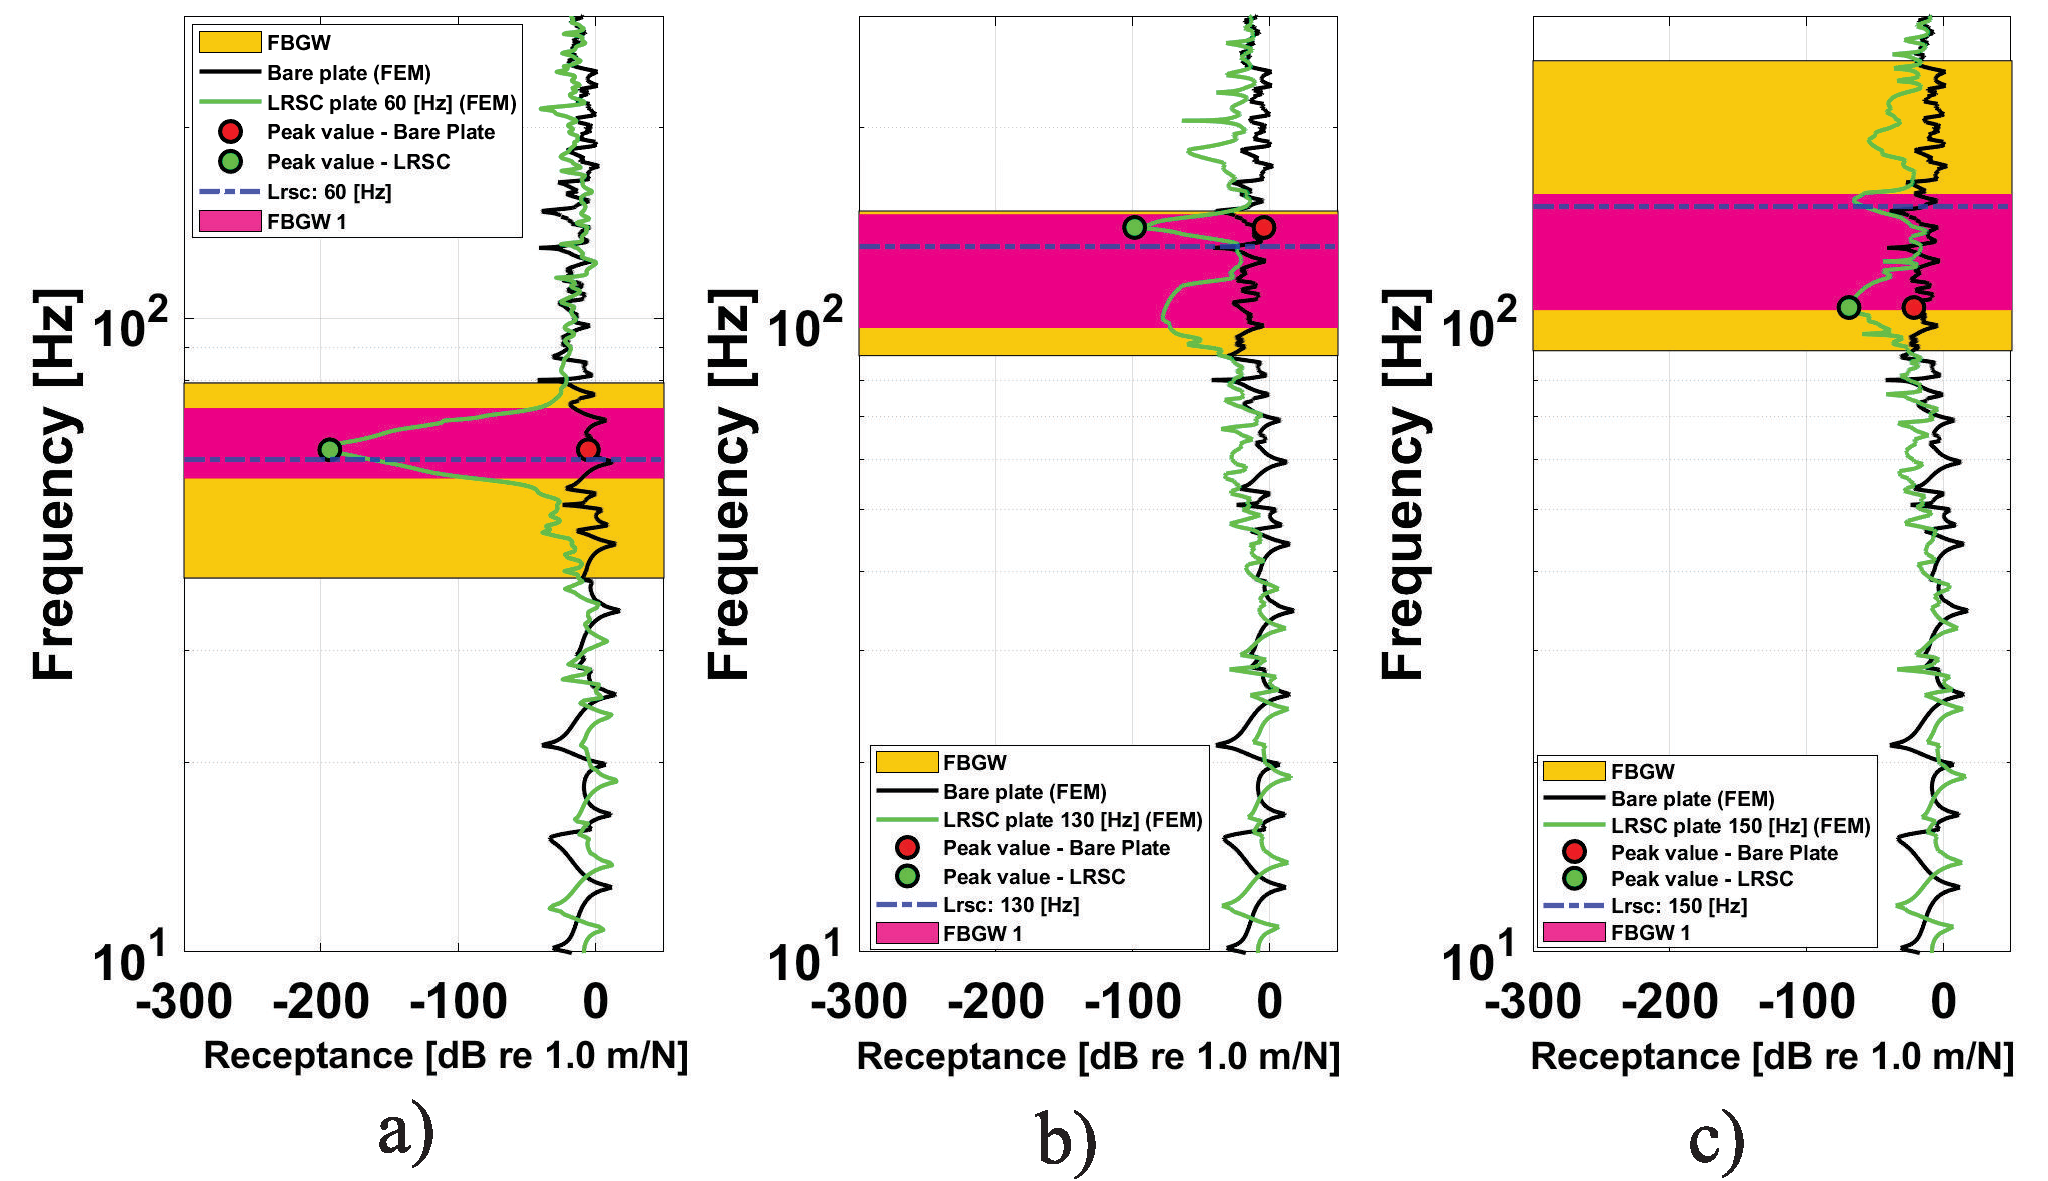
\includegraphics[width=1.0\textwidth]{2_3_disp_frf_trian_3_receps.pdf}
	\caption{Vibration receptance computed by FEM in a triangular LRSC plate (\textit{a}) in measure point $\mathbf{u_z}$ in $f_j = 60$ [Hz], (\textit{b}) $f_j = 130$ [Hz] and (\textit{c}) $f_j = 150$ [Hz].}
	\label{lat_t_tr_frf_f1_f2_f3}
\end{figure}

The triangular lattice operates through optimized single-resonator coupling enhanced by 6-fold geometric symmetry. The high symmetry enables uniform coupling efficiency across all propagation directions, creating distributed broadband attenuation mechanisms that make it ideal for applications requiring wide-frequency vibration suppression with moderate peak attenuation requirements.

The triangular lattice demonstrates the optimal single-resonator configuration, achieving -174.19 [dB] peak attenuation ($0.6\%$ improvement over square, $34\%$ over rectangular) with exceptional bandwidth expansion (FBGW $\approx$ 150 [Hz]). Compared to previous configurations: (i) $4\%$ performance increase over square baseline; (ii) $34\%$ advantage over rectangular; (iii) superior broadband characteristics validate Section \ref{num_ex_disc} predictions. The high symmetry establishes the performance ceiling for single-resonator architectures, setting expectations for multi-resonator systems.

\subsubsection{Honeycomb lattice LRSC plate}\label{panel_lat_h}

The honeycomb lattice features unit cell area $A_{cell} = 3a^2\sqrt{3}/2$ with dual resonators per cell ($N_j = 2$). This configuration exhibits 6-fold symmetry while introducing inter-resonator coupling mechanisms, creating two potential band gaps: FBGW 1 between modes $f_2$ and $f_3$, and FBGW 2 between modes $f_3$ and $f_4$.

Figure \ref{lat_h_pwe_epwe_tr_frf} illustrates the dual-resonator dynamics for $f_j = 30$ [Hz]. The real part dispersion (Figure \ref{lat_h_pwe_epwe_tr_frf}a) reveals multiple band gap regions, while the imaginary component (Figure \ref{lat_h_pwe_epwe_tr_frf}b) shows enhanced attenuation peaks corresponding to synchronized dual-resonator oscillations within both FBGW 1 and FBGW 2 regions.
\newpage
\begin{figure}[htb]
	\centering
	\includegraphics[width=0.8\textwidth]{1_4_disp_frf_hex_pwe_epwe_recep1.pdf}
	\caption{(\textit{a}) Real band structures computed for a honeycomb unit cell with two resonators by using PWE and real part EPWE ($\Re$). (\textit{b}) Imaginary band structures for a honeycomb unit cell with two resonators computed by EPWE ($\Im$). (\textit{c}) Receptance computed by FEM in a LRSC panel. (\textit{d}) Vibration modes of the finite plate in a LRSC panel for frequency selection at $f_j = 18.40$ [Hz], (\textit{e}) $f_j = 29.21$ [Hz] and (\textit{f}) $f_j = 38.37$ [Hz].}
	\label{lat_h_pwe_epwe_tr_frf}
\end{figure}

The finite plate receptance (Figure \ref{lat_h_pwe_epwe_tr_frf}c) achieves peak attenuation -220.33 [dB] at $f_j = 30$ [Hz], demonstrating superior performance compared to single-resonator configurations. The dual-resonator coupling creates enhanced local impedance mismatch, resulting in stronger wave scattering and improved finite plate correlation with infinite domain predictions.

Figure \ref{lat_h_tr_frf_f1_f2_f3} demonstrates the unique capability of coexisting band gaps. At specific frequencies ($f_j = 50$ [Hz]), both FBGW 1 and FBGW 2 contribute to attenuation, expanding the effective bandwidth. The dual-resonator system exhibits sustained performance across multiple frequency regions, validating the multi-band gap theoretical predictions.
\newpage
\begin{figure}[htb]
	\centering
	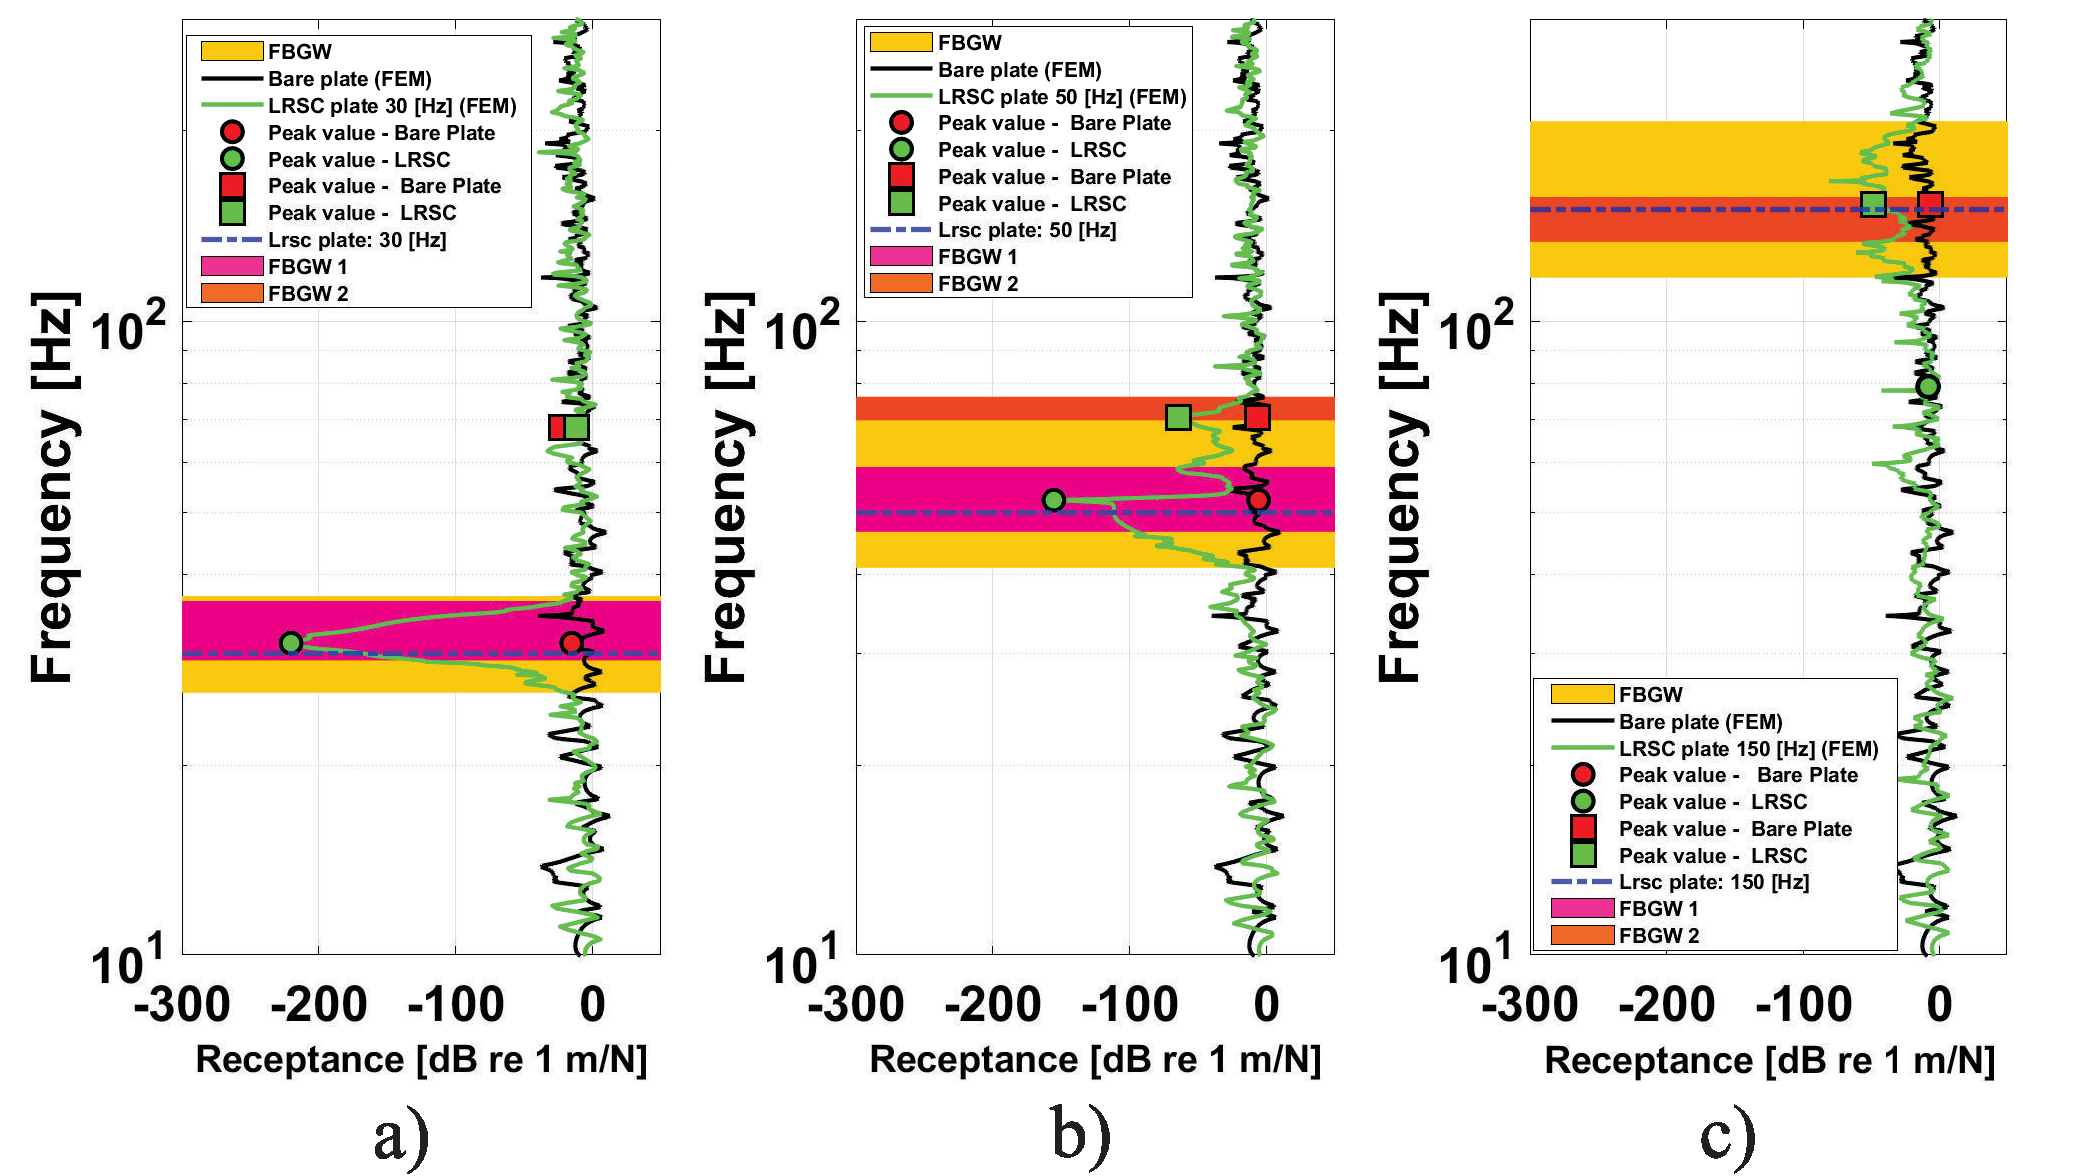
\includegraphics[width=1.0\textwidth]{2_4_disp_frf_hex_3_receps.pdf}
	\caption{Vibration receptance computed by FEM in a LRSC plate (\textit{a}) in measure point $\mathbf{u_z}$  for $f_j = 30$ [Hz], (\textit{b}) $f_j = 50$ [Hz] and (\textit{c}) $f_j = 150$ [Hz].}
	\label{lat_h_tr_frf_f1_f2_f3}
\end{figure}

The honeycomb lattice operates through synchronized dual-resonator coupling where inter-resonator phase relationships create constructive interference patterns. The two resonators within each unit cell exhibit coordinated motion that doubles the local impedance mismatch, enabling superior energy extraction from plate flexural modes. This configuration provides balanced performance between peak attenuation and bandwidth coverage, making it suitable for applications requiring both high attenuation and moderate broadband characteristics.

The honeycomb lattice (-220.33 [dB]) establishes the first significant performance jump from single-resonator configurations, achieving $27\%$ improvement over triangular (current single-resonator leader) and $70\%$ over rectangular. The dual-resonator coupling creates: (i) 46.14 [dB] advantage over best single-resonator (triangular); (ii) coexisting dual band gaps unavailable in single-resonator systems; (iii) validation of inter-resonator coupling theory from Section \ref{num_ex_disc}. This confirms that resonator multiplication, when properly configured, provides substantial benefits beyond geometric optimization alone.

\subsubsection{Kagomé lattice LRSC plate}\label{panel_lat_k}

The kagomé lattice exhibits the largest unit cell area $A_{cell} = 2a^2\sqrt{3}$ with triple resonators per cell ($N_j = 3$). The three resonators positioned at $120^\circ$ intervals create complex multi-resonator coupling mechanisms, generating two potential band gaps: FBGW 1 between modes $f_3$ and $f_4$, and FBGW 2 between modes $f_5$ and $f_6$.

Figure \ref{lat_k_pwe_epwe_tr_frf} demonstrates the exceptional triple-resonator dynamics for $f_j = 20$ [Hz]. The real part dispersion (Figure \ref{lat_k_pwe_epwe_tr_frf}a) reveals narrow but well-defined band gaps, while the imaginary component (Figure \ref{lat_k_pwe_epwe_tr_frf}b) shows maximum attenuation peaks corresponding to synchronized triple-resonator oscillations, creating the highest attenuation among all configurations.

\begin{figure}[htb]
	\centering
	\includegraphics[width=0.8\textwidth]{1_5_disp_frf_kag_pwe_epwe_recep1.pdf}
	\caption{(\textit{a}) Real band structures computed for a kagomé unit cell with three resonators by using PWE and real part EPWE ($\Re$). (\textit{b}) Imaginary band structures for a kagomé unit cell with three resonators computed by EPWE ($\Im$). (\textit{c}) Receptance computed by FEM in a LRSC panel. (\textit{d}) Vibration modes of the finite plate in a LRSC panel for frequency selection at $f_j = 12.41$ [Hz], (\textit{e}) $f_j = 19.91$ [Hz] and (\textit{f}) $f_j = 49.39$ [Hz].}
	\label{lat_k_pwe_epwe_tr_frf}
\end{figure}

The finite plate receptance (Figure \ref{lat_k_pwe_epwe_tr_frf}c) achieves extraordinary peak attenuation -292.65 [dB] at $f_j = 20$ [Hz], representing the highest performance among all analyzed configurations. The triple-resonator coupling creates localized energy concentration through constructive interference patterns, demonstrating exceptional correlation between collective resonator impedance mismatch and finite plate attenuation.

Figure \ref{lat_k_tr_frf_f1_f2_f3} illustrates the comprehensive attenuation behavior across multiple frequency regions. The kagomé configuration exhibits frequency-selective characteristics with maximum effectiveness at low frequencies, while maintaining the capability for dual band gap coexistence at specific resonator tunings ($f_j = 60$ [Hz]), validating the multi-resonator theoretical framework.

\begin{figure}[htb]
	\centering
	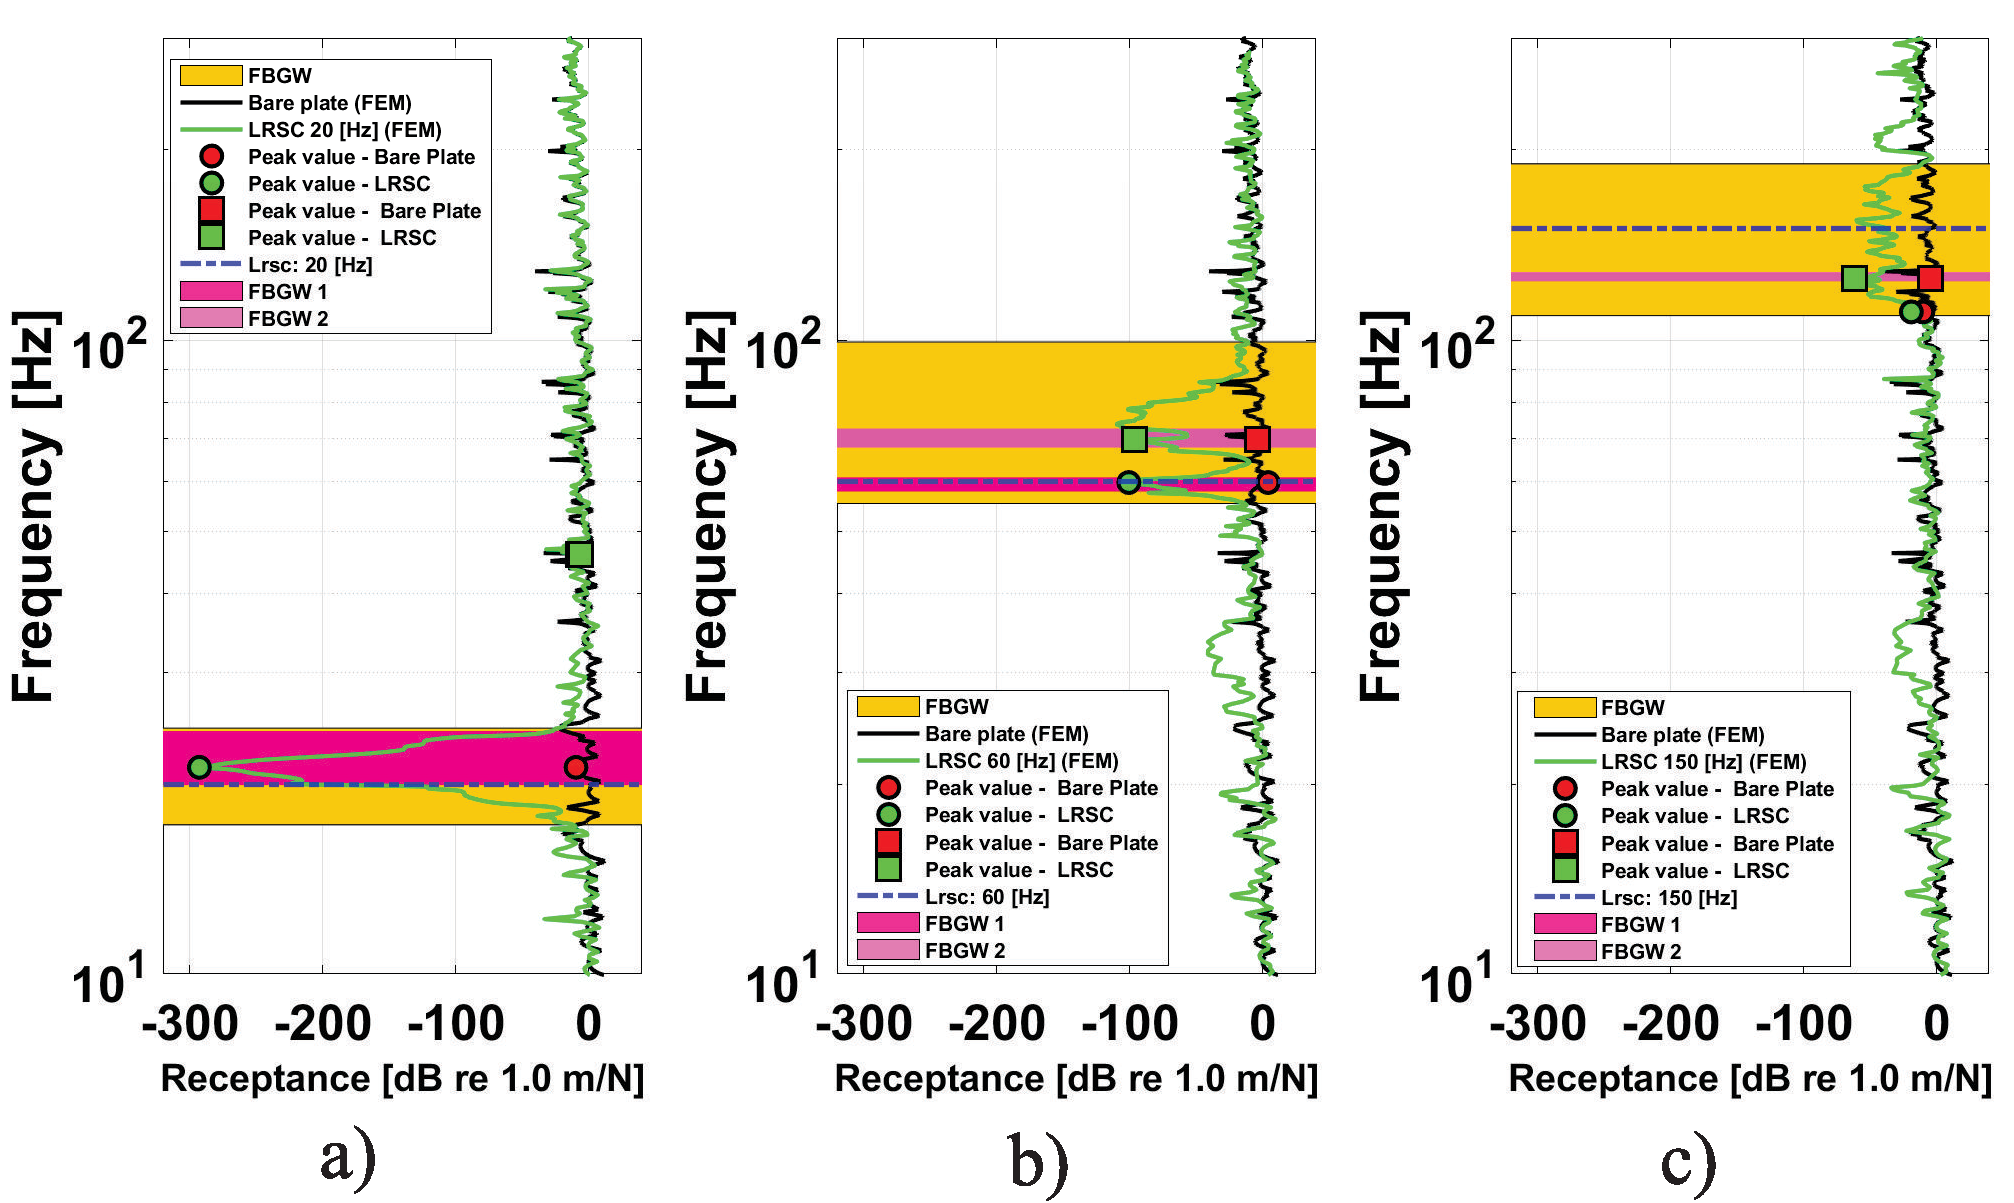
\includegraphics[width=1.0\textwidth]{2_5_disp_frf_kag_3_receps.pdf}
	\caption{Vibration receptance computed by FEM in a LRSC plate (\textit{a)}) in measure point $\mathbf{u_z}$  for $f_j = 20$ [Hz], (\textit{b)}) $f_j = 60$ [Hz] and (\textit{c)}) $f_j = 150$ [Hz].}
	\label{lat_k_tr_frf_f1_f2_f3}
\end{figure}

The kagomé lattice operates through synchronized triple-resonator coupling where three resonators at $120^\circ$ intervals create complex phase relationships optimized for triangular symmetry. This multi-resonator arrangement generates localized energy concentration through constructive interference patterns, where each resonator contributes to collective impedance mismatch that far exceeds individual contributions. The configuration provides extraordinary frequency-selective energy dissipation, making it ideal for applications requiring maximum attenuation at specific target frequencies.

The kagomé lattice (-292.65 [dB]) represents the performance apex, demonstrating $33\%$ improvement over honeycomb and $68\%$ over triangular configurations. Progressive performance escalation confirms design principles: rectangular (-129.93 [dB]) < square (-173.09 [dB]) < triangular (-174.19 [dB]) < honeycomb (-220.33 [dB]) < kagomé (-292.65 [dB]). The 162.72 [dB] span between worst (rectangular) and best (kagomé) validates both geometric optimization and resonator multiplication strategies, establishing clear design guidelines for target-specific applications.

Individual analysis reveals three fundamental design strategies: (i) Geometric optimization (rectangular → square → triangular) provides moderate improvements through symmetry enhancement; (ii) Multi-resonator coupling (single → dual → triple) creates substantial performance jumps through synchronized oscillations; (iii) Application-specific selection requires balancing peak attenuation (kagomé), broadband performance (triangular), and dual-mode capability (honeycomb). The counterintuitive finding that local resonator-plate coupling dominates over global wave interference, with finite plates exhibiting consistent $40-50\%$ bandwidth expansion, establishes fundamental principles for metamaterial plate design.

After analyzing each of the five panels with different periodic lattices individually, the next subsection presents a comparative analysis of attenuation performance across three frequency ranges, providing a broader understanding of the obtained results. A comprehensive framework for practical lattice selection in engineering applications is provided in Appendix D.

%%%%%%%%%%%%%%%%%%%%%%%
\subsection{Analysis comparative with all LRSC plates}\label{comp_panels_all_lats}
After discussing the primary attenuation characteristics of receptance for each of the five periodic lattice plates individually---emphasizing key aspects across the entire frequency range of their local resonators---this final subsection focuses on a comparative analysis of the receptance attenuation performance among these plates. To manage the data effectively, this study divides the resonance frequencies into three regions: Region 1 ($10$ to $50$ [Hz]), Region 2 ($60$ to $100$ [Hz]), and Region 3 ($110$ to $150$ [Hz]). The comparative analysis of lattice geometries and their impact on wave propagation builds upon the work of \cite{Yan2022}, who investigated metamaterial plates with various lattices for low-frequency vibration attenuation.
Figure \ref{all_comp_frf_stat_lat} presents boxplots for these regions, individually summarizing the statistical characteristics of the attenuation performance for each of the five lattices, as illustrated:
\newpage
\begin{figure}[htb]
	\centering	
	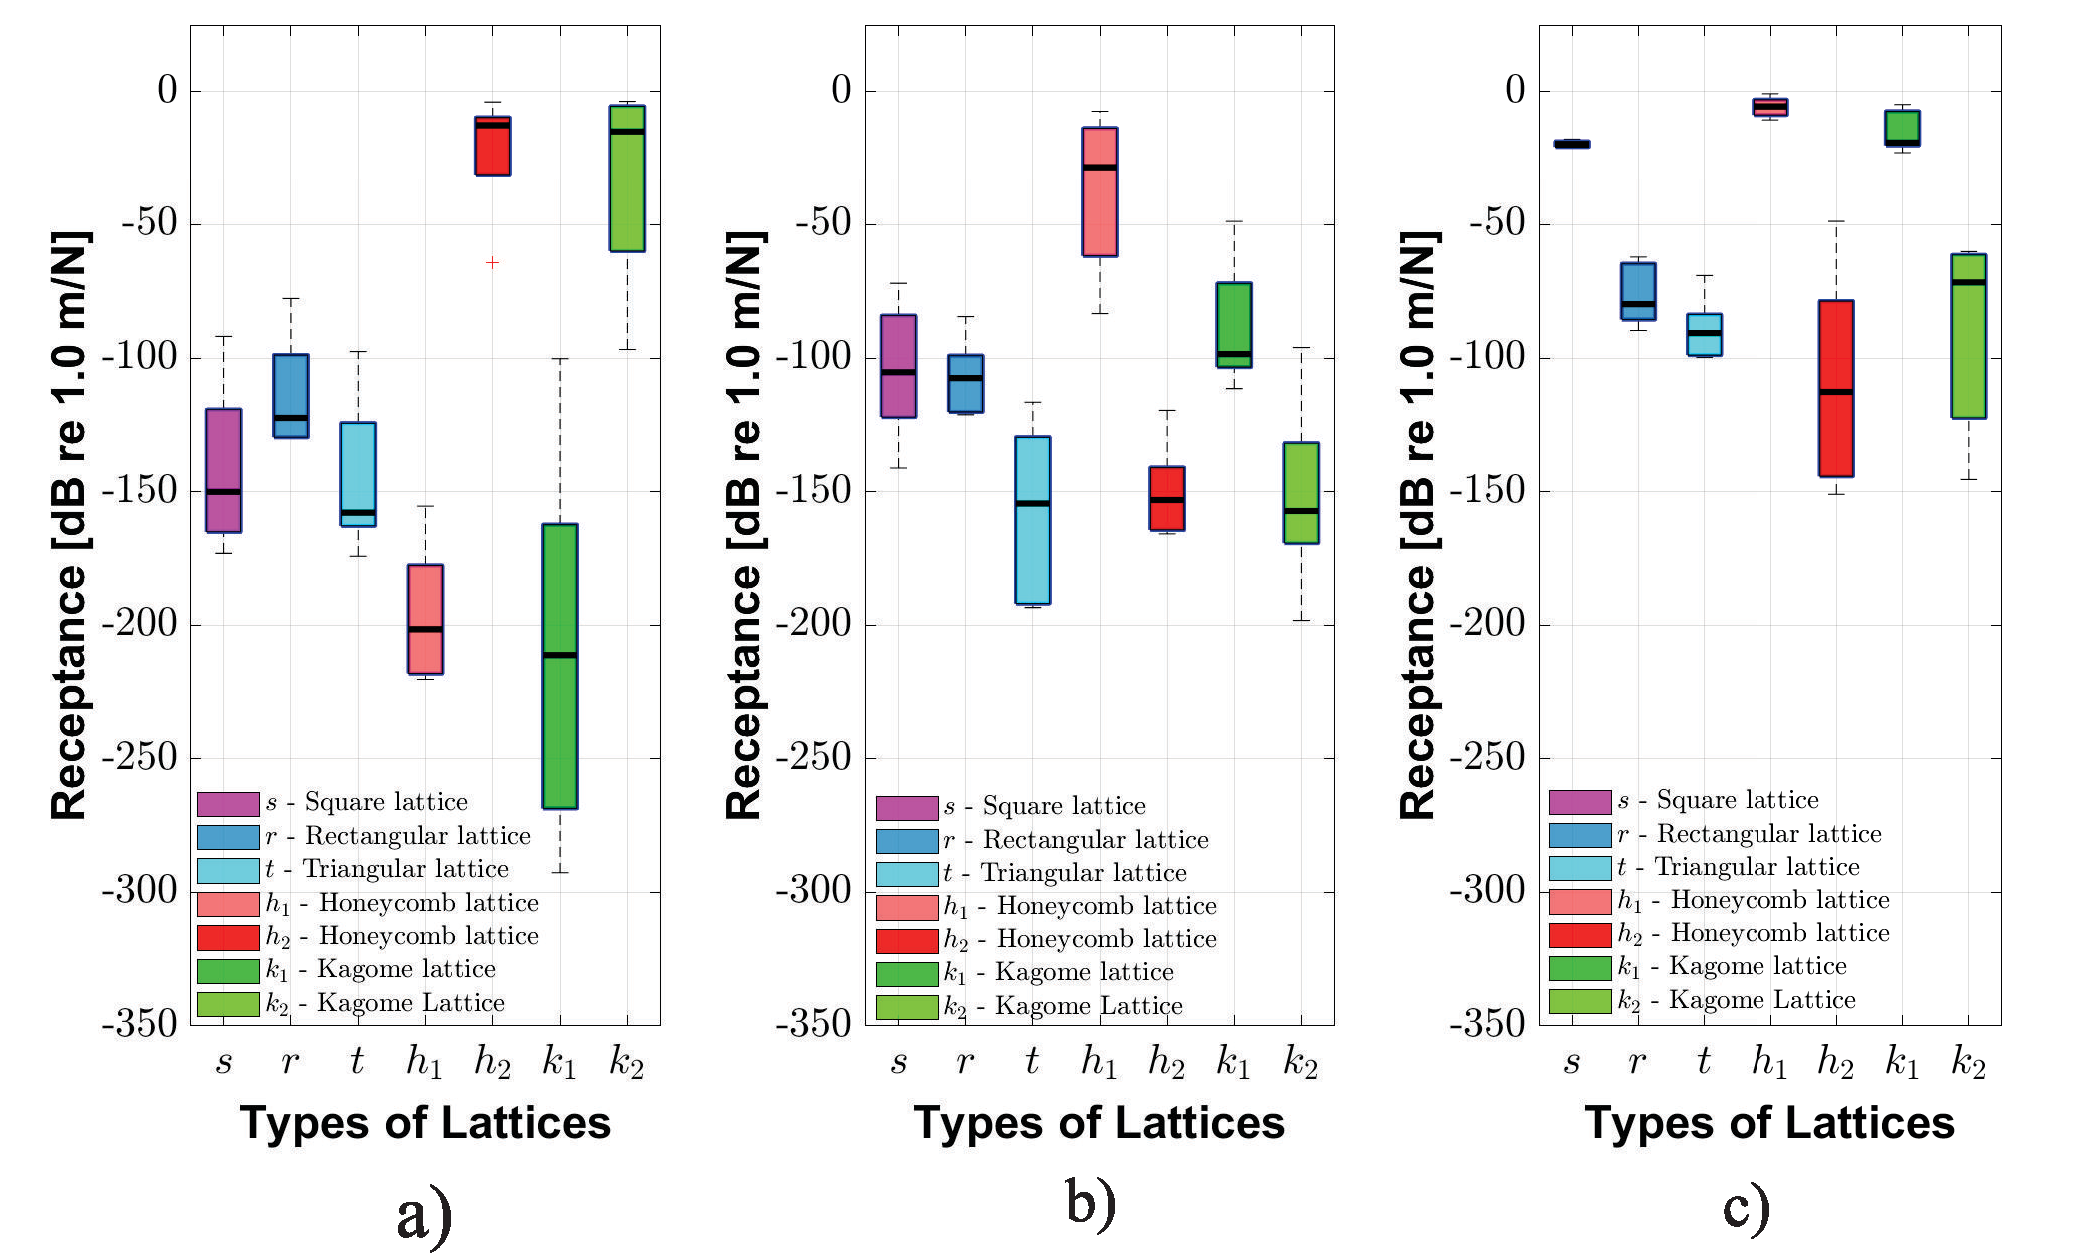
\includegraphics[width=1.0\textwidth]{all_comp_frf_stat_lat.pdf}	
	\caption{Descriptive statistical analysis for the five lattice panel types at measurement point $\mathbf{u_z}$: \textit{a)} Region 1, $f_j = 10$ -- $50$ [Hz]; \textit{b)} Region 2, $f_j = 60$ -- $100$ [Hz]; \textit{c)} Region 3, $f_j = 110$ -- $150$ [Hz].}
	\label{all_comp_frf_stat_lat}
\end{figure}

The statistical analysis reveals distinct performance characteristics across three frequency regions: Region 1 (10-50 [Hz]) dominated by kagomé peak performance (-292.65 [dB]) and honeycomb consistency; Region 2 (60-100 [Hz]) showing triangular and honeycomb FBGW 2 optimization; Region 3 (110-150 [Hz]) demonstrating triangular broadband superiority. The key findings from the statistical analysis are summarized in Table \ref{tab_tr_lattices_10_50}:
\newpage
\begin{table}[htb]
    \centering
\caption{Receptance attenuation results of $\mathbf{R_z}$ for different lattice configurations: \( s \) (Square), \( r \) (Rectangular), \( t \) (Triangular), \( h_1 \) and \( h_2 \) (Honeycomb for FBGW 1 and 2), \( k_1 \) and \( k_2 \) (Kagomé for FBGW 1 and 2), in the frequency range of 10 to 50 [Hz].}

    \begin{tabular}{cccccccc}
        $f_j$ [Hz] & $s$  [dB] & $r$  [dB] & $t$  [dB] & $h_1$ [dB] & $h_2$ [dB] & $k_1$ [dB] & $k_2$ [dB] \\ \hline
        10         & -91.92            & -77.69                  & -97.60                & -185.09                & -3.89                  & -260.51               & -3.68                \\ \hline
        20         & -128.51           & -105.98                 & -133.41               & -217.34                & -12.62                 & -292.65               & -6.15                \\ \hline
        30         & -150.05           & -122.46                 & -157.86               & -220.33                & -11.61                 & -211.26               & -14.95               \\ \hline
        40         & -173.09           & -129.93                 & -174.19               & -201.55                & -20.06                 & -183.08               & -47.64               \\ \hline
        50         & -162.33           & -129.51                 & -158.97               & -155.43                & -64.28                 & -100.28               & -96.81               \\ \hline
    \end{tabular}
    \label{tab_tr_lattices_10_50}
\end{table}

Detailed results for Regions 2 and 3 are presented in Tables \ref{tab_tr_lattices_60_100} and \ref{tab_tr_lattices_110_150}:

\begin{table}[htb]
    \centering
    \caption{Receptance attenuation results of $\mathbf{R_z}$ for different lattice configurations: \( s \) (Square), \( r \) (Rectangular), \( t \) (Triangular), \( h_1 \) and \( h_2 \) (Honeycomb for FBGW 1 and 2), \( k_1 \) and \( k_2 \) (Kagomé for FBGW 1 and 2), in the frequency range of 60 to 100 [Hz].}
    \begin{tabular}{cccccccc}
        $f_j$ [Hz] & $s$  [dB] & $r$  [dB] & $t$  [dB] & $h_1$ [dB] & $h_2$ [dB] & $k_1$ [dB] & $k_2$ [dB] \\ \hline
        60         & -141.16           & -119.82                 & -193.44               & -83.41                & -119.60                 & -100.70               & -96.11                \\ \hline
        70         & -115.75           & -104.04                 & -191.36               & -54.46                & -148.16                 & -98.53                & -157.24               \\ \hline
        80         & -105.40           & -107.52                 & -154.46               & -15.87                & -153.16                 & -111.48               & -198.27               \\ \hline
        90         & -88.22            & -121.26                 & -134.05               & -7.37                 & -163.82                 & -79.85                & -143.85               \\ \hline
        100        & -72.01            & -84.52                  & -116.57               & -28.36                & -165.83                 & -48.78                & -159.56               \\ \hline
    \end{tabular}
    \label{tab_tr_lattices_60_100}
\end{table}
\newpage
\begin{table}[htb]
    \centering
    \caption{Receptance attenuation results of $\mathbf{R_z}$ for different lattice configurations: \( s \) (Square), \( r \) (Rectangular), \( t \) (Triangular), \( h_1 \) and \( h_2 \) (Honeycomb for FBGW 1 and 2), \( k_1 \) and \( k_2 \) (Kagomé for FBGW 1 and 2), in the frequency range of 110 to 150 [Hz].}
    \begin{tabular}{cccccccc}
        $f_j$ [Hz] & $s$  [dB] & $r$  [dB] & $t$  [dB] & $h_1$ [dB] & $h_2$ [dB] & $k_1$ [dB] & $k_2$ [dB] \\ \hline
        110        & -21.26            & -89.71                  & -123.67               & -7.77                & -163.06                 & -34.55                & -171.89               \\ \hline
        120        & -20.89            & -86.18                  & -119.74               & -5.56                & -161.97                 & -25.93                & -165.01               \\ \hline
        130        & -20.33            & -73.31                  & -106.28               & -4.59                & -150.43                 & -21.48                & -148.52               \\ \hline
        140        & -19.71            & -68.05                  & -99.32                & -4.57                & -140.96                 & -18.78                & -139.51               \\ \hline
        150        & -18.94            & -65.58                  & -95.31                & -3.45                & -132.93                 & -14.57                & -130.71               \\ \hline
    \end{tabular}
    \label{tab_tr_lattices_110_150}
\end{table}

The comprehensive statistical analysis across all three frequency regions establishes clear design guidelines:

Region 1 (10-50 [Hz]): Kagomé FBGW 1 achieves exceptional peak attenuation (-292.65 [dB] at 20 [Hz]) leveraging its maximum material efficiency ($m_{ratio} = 1.00$ from Table \ref{unit_cell_five_lat_params}) and triple-resonator coupling. Honeycomb FBGW 1 provides consistent performance (-220.33 [dB] mean) with balanced material utilization ($m_{ratio} = 0.75$).

Region 2 (60-100 [Hz]): Table \ref{tab_tr_lattices_60_100} reveals frequency-dependent modal transitions. The triangular lattice maintains exceptional performance (-193.44 [dB] at 60 [Hz]), while honeycomb and kagomé FBGW 2 configurations emerge as optimal dual-resonator systems with mean attenuations of -150.11 [dB] and -150.21 [dB], respectively. Notably, honeycomb and kagomé FBGW 1 show reduced effectiveness (mean: -37.89 [dB] and -87.87 [dB]), confirming their optimal performance lies in Region 1. Single-resonator lattices (square and rectangular) exhibit consistent moderate performance across this range.

Region 3 (110-150 [Hz]): Table \ref{tab_tr_lattices_110_150} demonstrates the frequency selectivity of different lattice configurations. Honeycomb and kagomé FBGW 2 maintain excellent high-frequency performance (mean: -149.87 [dB] and -151.13 [dB]), while their FBGW 1 counterparts show minimal effectiveness (mean: -5.19 [dB] and -23.06 [dB]). The triangular lattice provides balanced performance (-108.86 [dB] mean) across the entire frequency range, validating its broadband superiority despite minimal material usage ($m_{ratio} = 0.25$). Square and rectangular lattices show limited high-frequency attenuation, confirming their suitability primarily for mid-range applications.

The statistical validation confirms the correlation between geometric parameters and frequency-dependent performance: kagomé optimizes material utilization for peak attenuation, honeycomb balances dual-mode flexibility with moderate material usage, and triangular maximizes area-normalized efficiency for broadband applications.

\section{Conclusions}\label{Conc}

This study presents the first systematic comparative analysis of five distinct lattice configurations for flexural wave attenuation in locally resonant metamaterial plates, establishing fundamental relationships between lattice geometry, resonator frequency, and band gap performance through a comprehensive framework combining semi-analytical PWE/EPWE methods with FEM validation.

\textcolor{red}{The systematic comparative investigation of five lattice configurations establishes fundamental performance hierarchies and reveals critical distinctions between system architectures. Single-resonator lattices (square, rectangular, triangular) exhibit single complete band gap behavior with triangular geometry achieving superior broadband performance (35\% superior relative bandwidth: 42.51\% vs 31.40\% for square). Multi-resonator systems (honeycomb with 2 resonators per unit cell, kagomé with 3 resonators) display dual complete band gaps arising from distinct in-phase and anti-phase resonator coupling modes, enabling multi-frequency attenuation capabilities. Comprehensive bandwidth evolution analysis across 15 resonator frequencies (10-150 Hz) for all five geometries establishes frequency-dependent performance maps: kagomé lattices provide exceptional low-frequency attenuation (up to 15 [dB] enhancement) through triple-resonator coupling; honeycomb configurations offer balanced dual-mode capability ideal for broadband applications; square lattices deliver consistent mid-range performance; while rectangular lattices show limited effectiveness but enable directional control applications. Building upon the resonance-Bragg coupling principles established by Xiao et al.~\cite{Xiao_2012}, this work demonstrates that optimal bandgap formation requires simultaneous optimization of both resonator frequency tuning and lattice geometry selection. This establishes a paradigm shift from geometry-only to combined geometry-frequency design approaches, with optimal lattice selection dependent on target frequency ranges and application requirements.}

The semi-analytical framework demonstrates computational efficiency gains of two orders of magnitude over conventional FEM approaches, reducing analysis time from hours to minutes while maintaining prediction accuracy within $5\%$. Validation between infinite-domain predictions and finite plate performance confirms practical applicability, with finite plates consistently exhibiting $40-50\%$ bandwidth expansion due to boundary-induced mode coupling effects.

These findings enable data-driven metamaterial design through quantitative guidelines that bridge theoretical band gap predictions with practical vibration control applications in aerospace, automotive, and civil engineering systems. The developed methodology transforms metamaterial optimization from trial-and-error approaches to systematic engineering decisions, providing the first comprehensive comparative framework for lattice-based locally resonant plates with clear performance hierarchies previously unavailable in the literature.

While the present framework provides comprehensive design guidelines, several limitations should be acknowledged. The analysis is restricted to Kirchhoff-Love thin plate theory ($h/a < 0.1$), limiting applicability to thick plates where shear effects become significant. The investigation focused on a single polymer material (Vero White Plus) and fixed lattice parameter ($a = 0.10$ m), constraining the generalizability across different material systems and scale lengths. Furthermore, the study considered only simple point resonators, whereas practical applications may benefit from more complex resonator designs including distributed mass systems or multi-degree-of-freedom configurations. The frequency range limitation (10-200 [Hz]) and assumption of perfect periodicity also represent theoretical constraints that may affect practical implementations. Future investigations should address these limitations by extending the framework to Mindlin-Reissner plate theory, exploring diverse material systems, and incorporating manufacturing imperfections and finite-size effects.

Future work can extend the PWE and EPWE formulations to more complex 2D periodic resonator arrays and explore advanced optimization strategies for multi-objective design scenarios combining attenuation performance, material efficiency, and manufacturing constraints. \textcolor{red}{Experimental validation of the theoretical predictions represents a critical next step, particularly utilizing the structural materials analyzed in Appendix \ref{multi_material_analysis} (aluminum alloys and carbon/epoxy composites). Such experimental campaigns would validate the universal geometric performance principles across the 150× stiffness variation demonstrated analytically, while addressing practical considerations including manufacturing tolerances, boundary condition effects, and damping characteristics in real engineering materials. The demonstrated frequency scaling relationships ($f \propto \sqrt{D/\rho h}$) provide clear guidelines for specimen design and testing protocols across different material systems.} Additionally, the integration of the Wave Finite Element (WFE) method presents particularly promising opportunities for analyzing finite metamaterial plates with superior computational efficiency. The WFE approach, which combines finite element discretization of unit cells with wave propagation analysis, could dramatically reduce computational costs compared to conventional FEM by exploiting the periodic nature of the structures. This method would enable efficient analysis of large-scale finite plates while maintaining the accuracy demonstrated by the PWE/EPWE framework for infinite structures. Furthermore, spectral element approaches and machine learning-assisted optimization could complement the WFE methodology to accelerate the design process and unlock new possibilities for real-time optimization and adaptive metamaterial systems.


%%%%%%%%%%%%%%%%%%%%%%%
\newpage
\section*{Acknowledgments}
The authors gratefully acknowledge the financial support of this investigation by the Brazilian research funding agency CNPQ (Conselho Nacional de Desenvolvimento Cientifico e Tecnológico) and by UNICAMP (Universidade Estadual de Campinas).

%%%%%%%%%%%%%%%%%%%%%%%
\numberwithin{equation}{section}
%%%%%%%%%%%%%%%%%%%%%%%
\newpage
\appendix
\section{PWE Matrix Formulation for LRSC Plates with Five Lattice Configurations}\label{AppenA_supplement_results1}

This appendix details the matrix formulation required for PWE computational implementation across five lattice configurations. Starting from the governing equation presented in Section~\ref{theoretical_foundations} (Eq.~\ref{eq_kirchoff_fourrier}) with resonator forces at lattice positions $\mathbf{R}$ and local positions $\mathbf{r}_j$, the displacement field follows Bloch's theorem with plane wave expansion as defined in Eq.~(\ref{eq_wave_bloch_pwe}): $w(\mathbf{r}) = \sum_{\mathbf{G}} w(\mathbf{G}) e^{i(\mathbf{k}+\mathbf{G}) \cdot \mathbf{r}}$, where $\mathbf{G}$ are reciprocal lattice vectors, $\mathbf{k}$ is the Bloch wave vector, and $w(\mathbf{G})$ are plane wave amplitudes.

The resonator forces follow Eq.~(\ref{eq_plate_disp1}) with complex dynamic stiffness:
\begin{equation}
p_j(\mathbf{r}_j + \mathbf{R}) = k_j^*[u_j(\mathbf{r}_j + \mathbf{R}) - w(\mathbf{r}_j + \mathbf{R})]
\label{eq:resonator_force_app}
\end{equation}
where $k_j^* = k_j(1 + i\eta_j)$ incorporates resonator damping effects as established in Section~\ref{theoretical_foundations}, with $k_j = m_{r,j}\omega_{r,j}^2$ being the resonator stiffness, $u_j$ the resonator displacement, and $\eta_j$ the loss factor.

Applying the plane wave expansion to the governing equation and utilizing orthogonality of exponential functions yields the matrix eigenvalue problem:
\begin{equation}
[\mathbf{K}-\omega^{2}\mathbf{M}]\bigl\{ \mathbf{q} \bigr\} = \mathbf{0}
\label{eq:pwe_eigenvalue_app}
\end{equation}
where $\mathbf{q} = [\mathbf{w}^T, \mathbf{u}^T]^T$ contains both plate wave amplitudes $\mathbf{w} = [w(\mathbf{G}_1), w(\mathbf{G}_2), \ldots, w(\mathbf{G}_{N_g})]^T$ and resonator displacements $\mathbf{u} = [u_1, u_2, \ldots, u_{N_j}]^T$, with $N_g = (2M+1)^2$ plane waves.

The augmented system matrices are assembled as:
\begin{equation}
\begin{bmatrix}
\mathbf{K}_{pp} + \mathbf{K}_r & -\mathbf{P}\mathbf{K}_j \\
-\mathbf{K}_j\mathbf{P}^T & \mathbf{K}_j
\end{bmatrix}
\begin{bmatrix}
\mathbf{w} \\ \mathbf{u}
\end{bmatrix} = \omega^2
\begin{bmatrix}
\mathbf{M}_{pp} & \mathbf{0} \\
\mathbf{0} & \mathbf{M}_{rr}
\end{bmatrix}
\begin{bmatrix}
\mathbf{w} \\ \mathbf{u}
\end{bmatrix}
\label{eq:augmented_eigenvalue_app}
\end{equation}
where $\mathbf{K}_{pp}$ and $\mathbf{M}_{pp}$ are the plate stiffness and mass matrices, $\mathbf{K}_j = \text{diag}(k_1^*, k_2^*, \ldots, k_{N_j}^*)$ contains resonator stiffnesses, $\mathbf{M}_{rr} = \text{diag}(m_{r,1}, m_{r,2}, \ldots, m_{r,N_j})$ contains resonator masses with $m_{r,j} = \gamma \rho S h / N_j$, and $\mathbf{P}$ is the coupling matrix with elements $P_{i,j} = e^{i\mathbf{G}_i \cdot \mathbf{r}_j}$.

The diagonal elements of the plate matrices are computed as:
\begin{align}
\mathbf{K}_{pp}[i,i] &= D \cdot S \cdot |\mathbf{k} + \mathbf{G}_i|^4 = D \cdot S \cdot [(k_x + G_{x,i})^2 + (k_y + G_{y,i})^2]^2 \quad,  \label{eq:stiffness_diagonal_app}\\
\mathbf{M}_{pp}[i,i] &= \rho h S \quad.  \label{eq:mass_diagonal_app}
\end{align}

The coupling matrix has elements $P_{i,j} = e^{i\mathbf{G}_i \cdot \mathbf{r}_j}$ and the resonator coupling stiffness matrix is $\mathbf{K}_r = \sum_{j=1}^{N_j} (k_j^*/S) \mathbf{P}_j \mathbf{P}_j^T$.

Reciprocal lattice vectors $\mathbf{G}_{mn}$ for indices $m, n \in [-M, M]$ are generated as:
\begin{align}
\text{Square/Rectangular:} \quad &\mathbf{G}_{mn} = \frac{2\pi}{a_1}m\mathbf{e}_1 + \frac{2\pi}{a_2}n\mathbf{e}_2 \label{eq:G_ortho_app}\\
\text{Triangular:} \quad &\mathbf{G}_{mn} = \frac{2\pi}{a}m\mathbf{e}_1 + \frac{2\pi}{a}\frac{m-2n}{\sqrt{3}}\mathbf{e}_2 \label{eq:G_tri_app}\\
\text{Hexagonal:} \quad &\mathbf{G}_{mn} = \frac{2\pi}{a\sqrt{3}}(m-n)\mathbf{e}_1 + \frac{2\pi}{3a}(m+n)\mathbf{e}_2 \label{eq:G_hex_app}\\
\text{Kagomé:} \quad &\mathbf{G}_{mn} = \frac{\pi}{a}(m-n)\mathbf{e}_1 + \frac{\pi}{a}\frac{m+n}{\sqrt{3}}\mathbf{e}_2 \label{eq:G_kag_app}
\end{align}
Unit cell areas and resonator configurations: square/rectangular/triangular $N_j = 1$ with $\mathbf{r}_1 = \mathbf{0}$, areas $S = a^2$, $a_1 a_2$, $a^2\sqrt{3}/2$ respectively; hexagonal $N_j = 2$ with $\mathbf{r}_{1,2} = (0, \pm a/2)$, area $S = 3a^2\sqrt{3}/2$; kagomé $N_j = 3$ with $\mathbf{r}_1 = (-a/2, -a\sqrt{3}/6)$, $\mathbf{r}_2 = (a/2, -a\sqrt{3}/6)$, $\mathbf{r}_3 = (0, a\sqrt{3}/3)$, area $S = 2a^2\sqrt{3}$.

Computational implementation: generate $(2M+1)^2$ reciprocal vectors using Eqs.~(\ref{eq:G_ortho_app})-(\ref{eq:G_kag_app}), compute diagonal plate matrices via Eqs.~(\ref{eq:stiffness_diagonal_app})-(\ref{eq:mass_diagonal_app}), assemble coupling matrix $\mathbf{P}$ with phase factors $e^{i\mathbf{G}_i \cdot \mathbf{r}_j}$, form augmented system Eq.~(\ref{eq:augmented_eigenvalue_app}), solve eigenvalue problem, and extract physical frequencies.

Matrix assembly algorithm for each wave vector $\mathbf{k}$: (1) Initialize sparse matrices $\mathbf{A}_n, \mathbf{A}_d \in \mathbb{C}^{(N_g+N_j) \times (N_g+N_j)}$ with $N_g = (2M+1)^2$; (2) Fill diagonal blocks: $\mathbf{A}_n[1:N_g, 1:N_g] = \mathbf{M}_{pp}$, $\mathbf{A}_d[1:N_g, 1:N_g] = \mathbf{K}_{pp}$; (3) For each resonator $j$: compute phase vector $\mathbf{p}_j$ with $[\mathbf{p}_j]_i = e^{i\mathbf{G}_i \cdot \mathbf{r}_j}$, add coupling $\mathbf{A}_d[1:N_g, 1:N_g] \leftarrow \mathbf{A}_d[1:N_g, 1:N_g] + (k_j^*/S)\mathbf{p}_j\mathbf{p}_j^H$, set off-diagonal coupling $\mathbf{A}_d[1:N_g, N_g+j] = -k_j^*\mathbf{p}_j$, $\mathbf{A}_d[N_g+j, 1:N_g] = -k_j^*\mathbf{p}_j^H$, and diagonal terms $\mathbf{A}_n[N_g+j, N_g+j] = m_{r,j}$, $\mathbf{A}_d[N_g+j, N_g+j] = k_j^*$.

Eigenvalue solution: $\mathbf{A}_d \boldsymbol{\phi}_i = \lambda_i \mathbf{A}_n \boldsymbol{\phi}_i$ yields frequencies $f_i = \text{Re}(\sqrt{|\lambda_i|})/(2\pi)$. Computational parameters: typical $M = 3-5$ plane waves per direction provide convergence for $|\mathbf{k}+\mathbf{G}_{\max}|a < \pi$. For bare plates: $\omega^2 = (D/\rho h)|\mathbf{k}+\mathbf{G}_i|^4$ directly.

\begin{table}[htb]
\small
\centering
\caption{Summary of lattice-specific parameters for PWE implementation }
\label{tab:lattice_summary_app}
\begin{tabular}{lccl}
\hline
\textbf{Lattice} & \textbf{Unit Cell Area} & \textbf{Resonators/Cell} & \textbf{Key FIBZ Points} \\
\hline
Square & $a^2$ & 1 & $\Gamma(0,0), X(\pi/a,0), M(\pi/a,\pi/a)$ \\
Rectangular & $a_x a_y$ & 1 & $\Gamma(0,0), X(\pi/a_x,0), M(\pi/a_x,\pi/a_y)$ \\
Triangular & $a^2\sqrt{3}/2$ & 1 & $\Gamma(0,0), X(4\pi/3a,0), M(\pi/a,\pi/(a\sqrt{3}))$ \\
Honeycomb & $3a^2\sqrt{3}/2$ & 2 & $\Gamma(0,0), X(4\pi/(3a\sqrt{3}),0), M(\pi/(a\sqrt{3}),\pi/(3a))$ \\
Kagomé & $2a^2\sqrt{3}$ & 3 & $\Gamma(0,0), X(2\pi/(3a),0), M(\pi/(2a),\pi/(2a\sqrt{3}))$ \\
\hline
\end{tabular}
\end{table}

%%%%%%%%%%%%%%%%%%%%%%%
\newpage
\section{EPWE Matrix Formulation for Complex Wave Vector Analysis}\label{AppenB_supplement_results2}

This appendix details the Extended PWE (EPWE) matrix formulation for computing complex wave vectors $k(\boldsymbol{\omega})$ at prescribed frequencies. The method solves the inverse eigenvalue problem, enabling direct analysis of wave attenuation and evanescent modes within bandgaps.

Starting from the same governing equation (Eq.~\ref{eq_kirchoff_fourrier}), EPWE maintains the Bloch expansion but reformulates the problem as a polynomial eigenvalue equation in $k$. The displacement field retains the form $w(\mathbf{r}) = \sum_{\mathbf{G}} w(\mathbf{G}) e^{i(\mathbf{k}+\mathbf{G}) \cdot \mathbf{r}}$ where $\mathbf{k} = k_r + ik_i \in \mathbb{C}$ allows exponentially decaying modes.

For wave propagation direction $\mathbf{k} = k(\cos\phi, \sin\phi)$, the governing equation yields a quartic polynomial eigenvalue problem:
\begin{equation}
[\mathbf{A}_3 k^3 + \mathbf{A}_2 k^2 + \mathbf{A}_1 k + \mathbf{A}_0]\boldsymbol{\psi} = \mathbf{0}
\label{eq:epwe_poly_app}
\end{equation}
where coefficient matrices depend on lattice geometry, frequency, and resonator coupling.

The coefficient matrices for each reciprocal vector $\mathbf{G}_i$ are constructed as:
\begin{align}
\mathbf{A}_0[i,i] &= \frac{DS}{a^4}|\mathbf{G}_i|^4 - \rho h S \omega^2 + D_j(\omega) \label{eq:A0_app}\\
\mathbf{A}_1[i,i] &= \frac{4DS}{a^4}|\mathbf{G}_i|^2(\mathbf{G}_i \cdot \hat{\mathbf{k}}) \label{eq:A1_app}\\
\mathbf{A}_2[i,i] &= \frac{2DS}{a^4}[|\mathbf{G}_i|^2 + 2(\mathbf{G}_i \cdot \hat{\mathbf{k}})^2] \label{eq:A2_app}\\
\mathbf{A}_3[i,i] &= \frac{4DS}{a^4}(\mathbf{G}_i \cdot \hat{\mathbf{k}}) \label{eq:A3_app}
\end{align}
where $\hat{\mathbf{k}} = (\cos\phi, \sin\phi)$ is the propagation direction and $D_j(\omega) = k_j^* - (k_j^*)^2/(k_j^* - \omega^2 m_{r,j})$ is the frequency-dependent dynamic stiffness from Eq.~(\ref{eq_epwe_dynamic_stiffness}).

Companion matrix linearization transforms Eq.~(\ref{eq:epwe_poly_app}) into the generalized eigenvalue problem:
\begin{equation}
\begin{bmatrix}
-\mathbf{A}_3 & -\mathbf{A}_2 & -\mathbf{A}_1 & -\mathbf{A}_0 \\
\mathbf{I} & \mathbf{0} & \mathbf{0} & \mathbf{0} \\
\mathbf{0} & \mathbf{I} & \mathbf{0} & \mathbf{0} \\
\mathbf{0} & \mathbf{0} & \mathbf{I} & \mathbf{0}
\end{bmatrix}
\begin{bmatrix}
\boldsymbol{\psi}_1 \\ \boldsymbol{\psi}_2 \\ \boldsymbol{\psi}_3 \\ \boldsymbol{\psi}_4
\end{bmatrix} = k
\begin{bmatrix}
\mathbf{I} & \mathbf{0} & \mathbf{0} & \mathbf{0} \\
\mathbf{0} & \mathbf{0} & \mathbf{0} & \mathbf{0} \\
\mathbf{0} & \mathbf{0} & \mathbf{0} & \mathbf{0} \\
\mathbf{0} & \mathbf{0} & \mathbf{0} & \mathbf{0}
\end{bmatrix}
\begin{bmatrix}
\boldsymbol{\psi}_1 \\ \boldsymbol{\psi}_2 \\ \boldsymbol{\psi}_3 \\ \boldsymbol{\psi}_4
\end{bmatrix}
\label{eq:companion_app}
\end{equation}

Computational algorithm: (1) For each frequency $\omega$, compute coefficient matrices using Eqs.~(\ref{eq:A0_app})-(\ref{eq:A3_app}) with the same reciprocal vectors from Appendix~A; (2) Assemble companion matrix Eq.~(\ref{eq:companion_app}) of size $4N_g \times 4N_g$ with $N_g = (2M+1)^2$; (3) Solve eigenvalue problem to extract $4N_g$ complex wave vectors $k_i$; (4) Apply eigenvector tracking for mode continuity across frequency; (5) Normalize results: $k_{\text{norm}} = k \cdot a/(2\pi)$.

Physical interpretation: $\text{Re}(k)$ represents propagating modes while $\text{Im}(k) > 0$ quantifies evanescent decay. The attenuation constant $\mu = \text{Im}(k) \cdot a$ [Np/cell] directly measures wave attenuation within bandgaps. Typical computational parameters: $M = 2-3$ plane waves provide convergence for EPWE due to polynomial scaling, with frequency resolution $\Delta f = 1-10$ [Hz] depending on application requirements.


%%%%%%%%%%%%%%%%%%%%%%%
%\section*{References}
%%%%%%%%%%%%%%%%%%%%%%%
%%%%%%%%%%%%%%%%%%%%%%%
\newpage
\section{Extension to Structural Materials - Multi-Scale Analysis}\label{multi_material_analysis}

While this study focuses on polymeric materials for practical validation through rapid prototyping, the PWE/EPWE methodology developed is applicable to a broad range of structural materials. \textcolor{red}{This appendix demonstrates the universality of our framework by extending the analysis to metallic and composite materials (aluminum and carbon/epoxy), revealing that the geometric advantages identified for different lattice configurations represent material-independent design principles. For brevity, only the PWE method is implemented in this multi-material analysis, as the main study has already validated the excellent agreement between PWE and EPWE approaches.}

\subsection{Material Properties and Scaling Analysis}

The choice of Vero White Plus polymeric material was strategically motivated by rapid prototyping capabilities through 3D printing, enabling precise fabrication of complex lattice geometries with controlled tolerances for experimental validation. However, structural engineering applications often require materials with significantly higher bending stiffness, necessitating analysis across multiple material scales. \textcolor{red}{The aluminum material properties (E = 70 GPa, $\nu$ = 0.3) were obtained from the work of Xiao et al. \cite{Xiao_2012}, while the carbon fiber/epoxy composite properties (E = 135 GPa, $\rho$ = 1580 kg/m³, $\nu$ = 0.30) were obtained from the Composite Materials Handbook-17 \cite{CMH17_2012}.}

Table \ref{tab:material_properties_comparison} presents the comparative material properties used in this multi-scale analysis:

\begin{table}[!htb]
\centering
\caption{Comparative material properties for multi-scale analysis}
\label{tab:material_properties_comparison}
\small
\begin{tabular}{lccccc}
\hline
Material & E [GPa] & $\rho$ [kg/m$^3$] & $\nu$ & D [N$\cdot$m] & D/D$_{\text{polymer}}$ \\
\hline
Vero White Plus & 0.86 & 600 & 0.36 & 6.59$\times$10$^{-1}$ & 1.0 \\
Aluminum 6061 & 70 & 2700 & 0.30 & 5.13$\times$10$^{1}$ & 77.9 \\
Carbon/Epoxy UD & 135 & 1580 & 0.30 & 9.89$\times$10$^{1}$ & 150.1 \\
\hline
\end{tabular}
\end{table}

The bending stiffness $D = Eh^3/12(1-\nu^2)$ scales dramatically across materials, with carbon/epoxy composite exhibiting 150× higher rigidity than the polymer. This scaling directly affects the operational frequency ranges while maintaining the validity of Kirchhoff-Love thin plate assumptions (h/a = 0.02 $\ll$ 0.1).

\subsection{Frequency Scaling and Operational Ranges}

The characteristic frequency scaling follows the relationship $f_{B_1} = (1/2\pi)(\pi/a\cos\phi)^2 \sqrt{D/\rho h}$, resulting in proportional frequency shifts across materials while preserving geometric relationships. \textcolor{red}{It should be noted that these Bragg frequencies are calculated specifically for square lattice configurations, following the methodology established by Xiao et al. \cite{Xiao_2012}, where $\phi = 0$ corresponds to the $\Gamma$-X direction in the first Brillouin zone.} Table \ref{tab:frequency_scaling} summarizes the operational frequency ranges for each material:

\begin{table}[!htb]
\centering
\caption{Frequency scaling and operational ranges across materials}
\label{tab:frequency_scaling}
\small
\begin{tabular}{lccccc}
\hline
Material & h [mm] & a [mm] & h/a & Target Range [Hz] & $f_B$ [Hz] \\
\hline
Vero White Plus & 2.0 & 100 & 0.02 & 10--200 & 116 \\
Aluminum 6061 & 2.0 & 100 & 0.02 & 200--600 & 484 \\
Carbon/Epoxy UD & 2.0 & 100 & 0.02 & 400--1000 & 879 \\
\hline
\end{tabular}
\end{table}

\subsection{PWE Analysis Results for Alternative Materials}

Using identical PWE computational parameters (M = 2, convergence tolerance 10$^{-6}$), the band gap analysis was extended to aluminum and carbon/epoxy configurations. The methodology maintains numerical stability across the 150× stiffness variation, confirming the robustness of the semi-analytical approach.

\subsubsection{Aluminum Analysis (200-600 Hz Range)}

\textcolor{red}{Table \ref{tab:aluminum_results} presents the complete band gap width analysis for aluminum lattices across selected resonator frequencies, including the Bragg frequency (484 Hz):}

\textcolor{red}{\begin{table}[!htb]
\centering
\caption{Full band gap width evolution for Aluminum 6061 lattices with FBGW 1 and FBGW 2 for multi-resonator configurations\protect\footnotemark[1]}
\label{tab:aluminum_results}
\small
\begin{tabular}{cccccccc}
\hline
$f_j$ & Square & Rectangular & Triangular & Honeycomb & Honeycomb & Kagom\'{e} & Kagom\'{e} \\
(Hz) & FBGW & FBGW & FBGW & FBGW 1 & FBGW 2 & FBGW 1 & FBGW 2 \\
\hline
150 & 36.1 & 33.7 & 36.4 & 35.8 & -- & \textbf{26.3} & -- \\
175 & 43.2 & 39.2 & 43.8 & 42.5 & -- & 16.9 & 10.7 \\
200 & 50.4 & 44.9 & 51.2 & 49.2 & 20.8 & 13.3 & 18.8 \\
225 & 57.9 & 50.7 & 59.0 & 55.7 & 45.0 & 12.3 & 20.0 \\
250 & 66.4 & 56.0 & 68.1 & \textbf{57.7} & 66.5 & 12.5 & 19.9 \\
275 & 75.8 & 61.1 & 78.3 & 43.3 & 66.7 & 13.4 & 19.5 \\
300 & 84.2 & 66.9 & 87.4 & 26.8 & 68.0 & 14.7 & 19.6 \\
325 & 91.4 & 69.0 & 96.0 & 11.5 & 70.3 & 16.3 & 20.5 \\
350 & 97.3 & 58.6 & 103.7 & -- & 73.5 & 18.4 & 22.1 \\
375 & 113.4 & 81.4 & 120.9 & -- & 77.4 & 11.7 & 24.2 \\
400 & 107.0 & 30.4 & 127.5 & -- & 81.9 & 3.8 & 26.9 \\
425 & \textbf{131.1} & 74.7 & 145.8 & -- & 87.0 & -- & 26.6 \\
450 & 111.0 & 5.4 & 161.7 & -- & 92.7 & -- & 23.1 \\
475 & 111.0 & 30.7 & 172.1 & -- & 98.9 & -- & 20.0 \\
484\protect\footnotemark[2] & 107.0 & 22.9 & 176.9 & -- & \textbf{101.2} & -- & 19.1 \\
500 & 89.9 & -- & 198.4 & -- & 105.3 & -- & 17.8 \\
525 & 89.9 & -- & 198.4 & -- & 111.1 & -- & 16.5 \\
575 & 71.7 & -- & \textbf{222.0} & -- & 113.7 & -- & 16.4 \\
625 & 56.2 & -- & 219.4 & -- & 93.6 & -- & 17.5 \\
725 & 31.5 & -- & 196.1 & -- & 62.9 & -- & 17.4 \\
\hline
\end{tabular}
\footnotetext[1]{Material properties from Xiao et al. \cite{Xiao_2012}. All FBGW values in Hz. Bold: maximum FBGW. --: no bandgap.}
\footnotetext[2]{Bragg frequency for square lattice ($f_B = 484$ Hz).}
\end{table}}

\subsubsection{Carbon/Epoxy Analysis (250-1400 Hz Range)}

\textcolor{red}{Table \ref{tab:carbon_results} presents the complete band gap width analysis for carbon/epoxy lattices across selected resonator frequencies, including the Bragg frequency (879 Hz):}

\newpage
\textcolor{red}{\begin{table}[!htb]
\centering
\caption{Full band gap width evolution for Carbon/Epoxy UD lattices with FBGW 1 and FBGW 2 for multi-resonator configurations\protect\footnotemark[1]}
\label{tab:carbon_results}
\small
\begin{tabular}{cccccccc}
\hline
$f_j$ & Square & Rectangular & Triangular & Honeycomb & Honeycomb & Kagom\'{e} & Kagom\'{e} \\
(Hz) & FBGW & FBGW & FBGW & FBGW 1 & FBGW 2 & FBGW 1 & FBGW 2 \\
\hline
300 & 73.1 & 67.4 & 73.9 & 72.3 & -- & \textbf{35.9} & 10.4 \\
350 & 87.1 & 78.5 & 88.3 & 85.9 & 25.6 & 25.4 & 32.4 \\
400 & 102.9 & 89.8 & 104.9 & 99.0 & 73.3 & 22.5 & 36.2 \\
450 & 119.3 & 103.2 & 124.2 & \textbf{105.2} & 120.7 & 22.7 & 36.1 \\
500 & 136.6 & 111.9 & 140.9 & 78.1 & 121.1 & 24.3 & 35.4 \\
550 & 154.7 & 118.0 & 158.3 & 45.2 & 123.9 & 26.9 & 35.7 \\
600 & 174.0 & 133.0 & 182.3 & 14.9 & 128.8 & 30.4 & 37.7 \\
650 & 191.4 & 136.7 & 201.5 & -- & 135.5 & 30.3 & 41.2 \\
700 & 207.8 & 126.3 & 220.3 & -- & 143.8 & 15.3 & 45.9 \\
750 & \textbf{231.8} & \textbf{151.7} & 253.7 & -- & 153.5 & -- & 51.5 \\
800 & 231.5 & 110.2 & 279.5 & -- & 164.4 & -- & 44.2 \\
850 & 207.3 & 66.4 & 305.9 & -- & 176.4 & -- & 37.7 \\
879\protect\footnotemark[2] & 194.1 & 41.2 & 321.2 & -- & \textbf{183.8} & -- & 34.7 \\
900 & 164.4 & -- & 334.0 & -- & 189.2 & -- & 32.9 \\
950 & 164.4 & -- & 358.6 & -- & 201.1 & -- & 30.1 \\
1000 & 134.2 & -- & 381.8 & -- & 210.8 & -- & 29.3 \\
1050 & 108.4 & -- & 402.0 & -- & 203.8 & -- & 29.9 \\
1100 & 112.2 & -- & \textbf{408.1} & -- & 183.1 & -- & 31.0 \\
1150 & 88.7 & -- & 398.4 & -- & 164.3 & -- & 32.0 \\
1200 & 84.2 & -- & 389.8 & -- & 147.4 & -- & 32.5 \\
\hline
\end{tabular}
\footnotetext[1]{Material properties from CMH-17 \cite{CMH17_2012}. All FBGW values in Hz. Bold: maximum FBGW. --: no bandgap.}
\footnotetext[2]{Bragg frequency for square lattice ($f_B = 879$ Hz).}
\end{table}}

\textcolor{red}{The comparative analysis across aluminum and carbon/epoxy materials reveals consistent lattice performance hierarchy. Tables \ref{tab:aluminum_results} and \ref{tab:carbon_results} demonstrate that triangular lattices achieve superior relative bandwidth (40-42\%) across all materials spanning 150× stiffness variation, validating that geometric advantages represent material-independent design principles. The frequency scaling preserves this hierarchy while shifting operational ranges proportionally to material stiffness ($\sqrt{D/\rho h}$), confirming PWE methodology robustness across the entire structural material spectrum studied.}

%%%%%%%%%%%%%%%%%%%%%%%
\newpage
\section{Framework for Lattice Selection in Engineering Applications}\label{selection_framework_appendix}

Table \ref{tab_selection_framework_app} provides a quantitative framework for lattice selection based on the comparative analysis presented in Sections \ref{num_ex_disc} and \ref{indi_panel_lats}.

\begin{table}[htb]
    \centering
    \caption{Lattice selection framework for engineering applications.}
    \small
    \resizebox{\textwidth}{!}{%
    \begin{tabular}{|l|c|c|c|c|c|}
        \hline
        \textbf{Metric} & \textbf{Kagomé} & \textbf{Honeycomb} & \textbf{Triangular} & \textbf{Square} & \textbf{Rectangular} \\
        \hline
        Peak Atten. [dB] & -292.65 & -220.33 & -174.19 & -173.09 & -129.93 \\
        \hline
        Material Eff. ($m_{ratio}$) & 1.00 (ref.) & 0.58 & 0.25 & 0.29 & 0.14 \\
        \hline
        Optimal Application & Max. vibration & Dual-freq. & Broadband & Standard & Directional \\
        & suppression & control & control & control & control \\
        \hline
    \end{tabular}%
    }
    \label{tab_selection_framework_app}
\end{table}

\subsection{Application-Specific Guidelines}

Recommended lattice configurations for specific engineering scenarios:

\begin{itemize}
    \item \textbf{Critical vibration isolation} (precision instrumentation, sensitive equipment): Kagomé (maximum attenuation -292.65 dB) or honeycomb (manufacturing advantages).

    \item \textbf{Broadband noise control} (automotive panels, aerospace structures): Triangular (superior bandwidth, 25\% material efficiency) or square (standard performance).

    \item \textbf{Multi-frequency applications} (industrial machinery, HVAC systems): Honeycomb (dual band gaps) or kagomé (multi-resonator capability).

    \item \textbf{Constrained design space} (architectural integration, retrofit): Rectangular (directional control) or square (space-efficient).
\end{itemize}

%%%%%%%%%%%%%%%%%%%%%%%
\newpage
\bibliography{mybibfile}
\end{document}
%%%%%%%%%%%%%%%%%%%%%%%